Tato kapitola se zabývá samotnou realizací platformy pro měření odpracovaného času. Popisuje nástroje použité během vývoje, strukturu zdrojového kódu a~nakonec implementaci jednotlivých navržených funkcionalit aplikace.

%---------------------------------------------------------------
\section{Nástroje pro vývoj}\label{development-tools}
%---------------------------------------------------------------

Jak bylo navrženo v~sekci \ref{dev-tools}, pro nativní aplikaci bylo použito vývojové prostředí \emph{Xcode}. Verze tohoto IDE, na kterém byla implementace vyvíjena, byla 15.2. S~touto verzí IDE se pojí verze programovacího jazyku \emph{Swift} 5.9.2. Aplikace byla vyvíjena na operačním systému \emph{macOS Sonoma} (14.4). Nativní aplikace bude definovat minimální iOS verzi cílové platformy na verzi 17.0, jelikož tato verze umožňuje použití nejnovějších nástrojů platformy iOS. Podle dat z~února 2024 už tuto nejnovější verzi operačního systému používalo 66\% ze všech aktivních uživatelů mobilních telefonů iPhone. Mezi zařízeními představených v~předchozích čtyřech letech je to dokonce 76\% \cite{ios-17-adoption}.

Vývojové prostředí pro multi-platformní část a~backend také dodržuje návrh ze sekce \ref{dev-tools}, bylo tedy použito \emph{IntelliJ IDEA}, verze 2024.1. Pro jazyk \emph{Kotlin} byla použita verze 1.9.10. 
 a~
\emph{Git} repozitář byl zálohován nástrojem \emph{GitHub} \cite{github} v~repozitáři \cite{trackee-app-github}. Během vývoje nebyly použity žádné větve ani další nástroje pro týmovou spolupráci v~nástroji \emph{Git}, jelikož nikdo další na projektu nespolupracoval. Veškerý vývoj tedy probíhal přímo v~hlavní větvi \emph{main}.

%---------------------------------------------------------------
\subsection{Firebase}
%---------------------------------------------------------------

V~nástroji \emph{Firebase}, který byl vybrán v~návrhu v~sekci \ref{platform-architecture}, byl vytvořen projekt pro aplikaci Trackee. Byly vytvořeny tři prostředí – Alpha, Beta a~Produkce. V~projektu zatím byly nastaveny funkce pro autentizaci a~\emph{Firestore} databázi. 

\emph{Firebase} autentizace podporuje různé formy autentizace, jako e-mail s~heslem, ale třeba také přihlášení přes Google, přes Apple, přes Facebook a~podobně. Rozšíření možností přihlášení by mohlo být podnětem pro budoucí vývoj aplikace, v~této fázi je zatím implementováno pouze přihlášení přeš e-mail a~heslo. 

Při tvorbě \emph{Firestore} databáze \emph{Firebase} nabízí výběr, kde se má instance databáze nacházet (západní Evropa nebo Severní Amerika). Byla vybrána nejbližší možnost, tedy západní Evropa.

%---------------------------------------------------------------
\subsection{Nasazení backendu}\label{backend-deployment}
%---------------------------------------------------------------

Během vývoje byla aplikace backendu spouštěna a~testována na lokálním stroji. V~místních sítích se tedy stačilo připojovat pomocí IP adresy počítače, na kterém aplikace backendu běžela, přes protokol HTTP, například: \texttt{http://192.168.88.70:8080}

Pro umožnění používání aplikace kdekoli, kdykoli a~bez potřeby na lokálním stroji neustále ručně spouštět aplikaci backendu, bylo vhodné vybrat nějaké řešení, které by umožnilo nasazení aplikace backendu. K~tomu existuje řada externích poskytovatelů. Pro potřeby tohoto projektu byl zvolen nástroj \emph{Railway} \cite{railway}, jelikož zdarma nabízí počáteční kredit v~hodnotě pěti amerických dolarů, což by mělo na nějakou dobu vystačit pro potřeby vývoje aplikace. Tomuto nástroji pouze stačí propojení s~\emph{GitHub} repozitářem, nastavení skriptu pro spuštění a~je hotovo. Nástroj poté při každé aktualizaci repozitáře sestaví projekt, spustí backend a~nasadí ho na URL adrese \texttt{https://trackee-app-production.up.railway.app}. 

\emph{Railway} také podporuje automatické uspávání aplikace, které může snížit využívání kreditu v~době, kdy aplikace není využívána \cite{railway-app-sleeping}. Pokud se tedy aplikace nějakou dobu nepoužívá, je potřeba počítat s~několika sekundovou prodlevou při prvním požadavku.

Jednou nevýhodou nástroje \emph{Railway} ale je, že v~bezplatné variantě nabízí umístění stroje, na kterém běží instance, pouze ve státě Oregon ve Spojených státech amerických. Jelikož je to v~podstatě na druhé straně Země, vzniká tím poměrně znatelná prodleva mezi klientem a~serverem. A~v~kombinaci s~tím, že při nastavení nástroje \emph{Firebase} bylo zvoleno umístění instance v~Evropě (a toto umístění není možné po nastavení nástroje změnit), vznikají tím hlavně prodlevy při komunikaci s~databází, protože nyní musí backend každý požadavek na čtení nebo zápis dat posílat zhruba 8 tisíc kilometrů daleko. Rozdíl mezi používáním instance backendu běžící pomocí nástroje \emph{Railway} a~používáním lokální instance je znatelný – například přihlášení a~načtení hlavní obrazovky včetně plné počáteční stránky historie záznamů (10 záznamů) trvá 5-7 sekund, zatímco při použití lokální instance toto trvá 2-3 sekundy.

%---------------------------------------------------------------
\subsection{Nasazení aplikace a~Testflight}\label{testflight}
%---------------------------------------------------------------

Vývojové prostředí \emph{Xcode} umožňuje nahrání vyvíjené aplikace do připojeného mobilního zařízení. Dané zařízení ale musí být fyzicky připojeno k~počítači, na kterém IDE běží, musí být ve vývojářském režimu a~musí být napojené na vývojářský účet, pod který aplikace spadá. Jedná se tedy o~poměrně komplikované řešení, je-li účelem instalace aplikace mezi další uživatele, například mezi testery.

Nástrojem, jak řešit nasazení aplikace mezi širší počet uživatelů, ale nikoli zatím jako finální aplikaci mířenou na reálné uživatele, je \emph{Testflight} \cite{testflight}. Tento nástroj je určen pro beta testování vyvíjených aplikací. Umožňuje nahrávání archivovaných (sestavených) aplikací pomocí nástroje \emph{App Store Connect} \cite{app-store-connect} a~jejich následnou distribuci mezi vybrané uživatele, kteří si tuto aplikaci nainstalují. Jsou dva způsoby, jak lze aplikace přes \emph{Testflight} distribuovat:
\begin{itemize}
\item\textbf{Interní testování} – vývojář pozve jednotlivé uživatele pomocí jejich e-mailové adresy k~testování aplikace a~ti si ji mohou stáhnout. Tito vývojáři musí mít účet \emph{Apple ID} a~musí být přidání mezi interní vývojáře aplikace.
\item\textbf{Veřejné testování} – vývojář může do testování přizvat kohokoli, dokonce stačí jenom takzvaný \emph{public link}, přes který si uživatelé mohou aplikaci nainstalovat. Aby aplikace mohla být testována pomocí veřejného testování, musí být schválena firmou \emph{Apple} v~rámci procesu \emph{App Review}, který aplikace podstupují i~tehdy, pokud chtějí zamířit mezi reálné uživatele do obchodu \emph{App Store}.
\end{itemize}

Aplikace Trackee umožňuje oba typy testování, již prošla schvalovacím procesem \emph{App Review} a~může si ji tak nainstalovat kdokoli, kdo bude pozvaný přes e-mailovou adresu, nebo pomocí \emph{public linku}: \texttt{https://testflight.apple.com/join/cTRdRkBc}

%---------------------------------------------------------------
\section{Architektura a~struktura projektu}\label{project-structure}
%---------------------------------------------------------------

Jako šablona celého projektu sloužil \emph{DevStack} společnosti \emph{Matee} \cite{matee-devstack}, ze kterého byla odstraněna většina implementovaných funkcionalit a~jejich balíčků, kromě těch, které se hodilo znovu využít (onboarding, profil, \dots). Ze šablony byly také ponechány nástroje na síťovou komunikaci (síťový klient pomocí knihovny \emph{Ktor} \cite{ktor}), interoperabilitu a~další. V~šabloně také byly ponechány některé nástroje, které zatím projektem nejsou využívány, ale v~budoucnu při dalším rozvoji aplikace by se mohly hodit, jako nástroje pro práci s~lokálním úložištěm \emph{SQLDelight}, \emph{UserDefaults} nebo \emph{Keychain}, nebo \emph{Providers} pro obsluhu GPS, obsluhu notifikací, a~další. Jelikož Aplikace Trackee neimplementuje Android klienta, je celý jeho modul ze šablony odstraněn.

Aplikace implementuje tři prostředí – Alpha, Beta a~Produkce. Zvykem bývá, že Alpha má vlastní instanci databáze a~serveru, která slouží pouze pro testování a~ladění, například při nasazování nových verzí backendu, a~podobně. Beta na tom je pak obvykle podobně, ale buď duplikuje data z~produkčního prostředí (ale přímo ho nemůže ovlivňovat), nebo je na produkční prostředí přímo napojena, ale nabízí přidané ladící možnosti. Produkční prostředí pak poskytuje databázi a~server, které jsou využívány reálnými uživateli, kde je priorita orientována spíše na rychlost, než na možnosti ladění. Během vývoje aplikace Trackee nebylo potřeba využívat více instancí databáze nebo serveru, protože na projektu nepracuje více lidí, nevznikají konflikty a~není zatím využíván reálnými uživateli. Prostředí se tedy liší jenom v~drobnostech, jako například v~tom, že Alpha a~Beta nabízí rozšířené možnosti zachycování a~přepisování požadavků na backend, nebo poskytuje detailnější popisy chybových hlášek, které mohou obsahovat více technických informací. 

Multi-platformní část a~backend používají automatizační sestavovací nástroj \emph{Gradle} \cite{gradle}, což je populární nástroj pro flexibilní konfiguraci a~automatizaci sestavování softwarových projektů. Nativní iOS aplikace používá pro sestavení nástroj \emph{xcodebuild}, který je součástí \emph{Xcode} IDE. Multi-platformní knihovna je do nativní iOS aplikace propagována jako knihovna typu \emph{xcframework}, což je \emph{multiplatformní binární framework} \cite{xcframework}. \emph{Gradle} zkompiluje multi-platformní kód do této \emph{xcframework} reprezentace a~zkopíruje ji do iOS projektu.

Implementace API backendové části aplikace dodržuje návrhové vzory \emph{REST} \cite{rest-api}, jedná se tedy o~\emph{RESTful API}. Pro možnosti rozšiřovatelnosti aplikace nabízí \emph{Swagger OpenAPI} dokumentaci \cite{swagger-open-api} na URL adrese \texttt{<backend-host-url>/openapi}, v~případě nasazení v~\emph{Railway} aplikaci tedy na URL adrese \texttt{https://trackee-app-production.up.railway.app/openapi}. Zdrojem této dokumentace je soubor \texttt{openapi/documentation.yaml} ve složce \texttt{resources} ve zdrojovém kódu aplikace backendu.

Všechny části implementace (nativní aplikace, multi-platformní část a~backend) jsou součástí jednoho repozitáře (\emph{monorepo}), který má následující strukturu:
\begin{itemize}
\item\texttt{backend} – modul obsahující projekt backendu
\item\texttt{build-logic} – společný modul ostatních modulů, obsahující pluginy a~nástroje pro sestavení multi-platformní knihovny
\item\texttt{gradle} - složka pro soubory nástroje \emph{Gradle}
\item\texttt{ios} – složka obsahující projekt nativní iOS aplikace
\item\texttt{other} – nástroje projektu
\item\texttt{shared} – modul obsahující sdílený kód pro technologii \emph{Kotlin Multiplatform}
\item\texttt{twine} – složka obsahující lokalizační soubor
\end{itemize}
Jednotlivé části implementace poté dodržují architekturu navrženou v~sekci \ref{platform-architecture}.

%---------------------------------------------------------------
\subsection{Lokalizace}
%---------------------------------------------------------------

Aplikace byla implementována a~lokalizována pro tři jazyky – čeština, slovenština a~angličtina. Zdroje pro lokalizace všech textů (tlačítka, popisky, instrukce, \dots) jsou uloženy v~souboru \texttt{strings.txt} ve složce \texttt{twine}, který je připraven ve formátu pro nástroj \emph{Twine} \cite{twine}, který tento soubor zpracovává a~tvoří z~něj lokalizační soubory pro cílové platformy (pro iOS jsou to soubory \texttt{Localizable.strings}). Nastavení tohoto nástroje pro tyto jazyky je již v~šabloně \emph{DevStack} připraveno.

%---------------------------------------------------------------
\subsection{Automatické generování kódu}
%---------------------------------------------------------------

Šablona také používá několik pomocných nástrojů pro automatické generování kódu. Jedním takovým nástrojem je \emph{SwiftGen} \cite{swiftgen}, který zde slouží k~několika účelům:
\begin{itemize}
\item Generování struktur pro lokalizaci: \emph{SwiftGen} podle šablon generuje statické struktury z~lokalizačních souborů \texttt{Localizable.strings} pro jednodušší použití v~kódu, které zamezí použití špatných klíčů lokalizací.
\item Generování struktur pro obrázky: \emph{SwiftGen} je v~šabloně nastaven takovým způsobem, aby ze zdrojů \texttt{Images.xcassets} generoval statické struktury, které umožní jednodušší referování obrázků ze zdrojového kódu.
\item Generování struktur pro barvy: Funguje stejným způsobem, jako obrázky.
\end{itemize}
Nástroj \emph{SwiftGen} je v~šabloně přidán jako \emph{plugin} modulu \emph{UIToolkit} v~prezentační vrstvě.

Nativní iOS aplikace také v~šabloně využívá makra \emph{swift-spyable} \cite{swift-spyable} \emph pro generování \emph{Use Case Mocks}, tedy statických náhrad pro \emph{Use Cases} používaných pro testování. Toto je ale používáno jen pro nativní \emph{Use Cases}, které aplikace Trackee neobsahuje. Pro sdílené \emph{Use Cases} je využíváno vlastních rodičovských tříd \texttt{UseCaseResultMock}, \texttt{UseCaseResultNoParamsMock}, atd.

%---------------------------------------------------------------
\subsection{Dependency Injection}
%---------------------------------------------------------------

Pro \emph{Dependency Injection} v~nativní aplikaci je využíváno knihovny \emph{Factory} \cite{factory}, v~multi-platformní části a~na backendu knihovny \emph{Koin} \cite{koin}. V~aplikaci Trackee jsou sice všechny \emph{Use Cases} a~\emph{Repositories} v~multi-platformní části, ale \emph{Dependency Injection} v~prezentační vrstvě nativní aplikace získává implementace sdílených \emph{Use Cases} knihovnou \emph{Factory}, aby bylo dosazování sjednocené s~případnými nativními \emph{Use Cases}. \emph{Dependency Injection} v~nativní aplikaci tedy funguje tak, že v~modulu \emph{DependencyInjection} v~aplikační vrstvě se registrují implementace všech závislostí, včetně sdílených \emph{Use Cases}, které ale poskytuje knihovna \emph{Koin}.

%---------------------------------------------------------------
\section{Implementace jednotlivých funkcionalit}
%---------------------------------------------------------------

Tato sekce se věnuje implementaci jednotlivých funkcionalit navržených v~sekci \ref{features}. Implementaci každé funkcionality rozebírá z~hlediska její realizace v~backendové části, v~multi-platformní části a~v~nativní aplikaci. 

U~jednotlivých funkcionalit mohou být uvedeny ukázky výpisů kódu, většinou tak, aby pro každou funkcionalitu byl ukázán příklad zdrojového kódu z~jiné části aplikace. Cílem je poskytnout pár příkladů pro představu toho, jakým stylem je zdrojový kód implementován, a~ne zbytečně ukazovat výpisy kódů pro věci, které jsou velmi podobné implementaci, která již byla ukázána v~jiné části. Pro důkladnější studium kódu samozřejmě slouží zdrojový kód sám, který je součástí přiloženého média této práce. Text této práce slouží mimo jiné jako jeho dokumentace, která v~něm má usnadnit orientaci.

%---------------------------------------------------------------
\subsection{Přihlášení a~registrace}\label{onboarding-impl}
%---------------------------------------------------------------

Přihlášení a~registrace je základní funkcionalitou, kterou aplikace potřebuje, aby mohla držet informace o~konkrétním uživateli. V~návrhu platformy (obrázek \ref{fig:architecture}) byla autentizace navržena tak, že bude probíhat přes backend. Ale vzhledem k~tomu, že \emph{Firebase} autentizace nabízí více možností autentizace, jako přihlášení přes Apple, Google, a~podobně, tak byl v~implementaci zvolen přístup, že autentizace bude probíhat na straně klienta, a~ne backendu, protože jí celou obstará \emph{Firebase} autentizace. Bylo by sice možné provádět autentizace přes e-mail a~heslo tak, že by klient poslal danou kombinaci e-mailu a~hesla na backend, který by uživatele přes \emph{Firebase} přihlásil, klientovi vrátil jeho \emph{access token}\footnote{\emph{Access token} je v~autentizační terminologii řetězec znaků, se kterým klient posílá požadavky na server, aby prokázal svou identitu. \cite{access-token}}, který by ho poté dále používal při následujících požadavcích. V~případě rozšíření o~další formy přihlášení, jako je přihlášení přes Apple, by v~tomto přístupu musel \emph{Firebase} provést autentizaci u~klienta, získat mezistavový \emph{token} pro daného poskytovatele přihlášení, poslat ho na backend, který by ho poté ověřil s~autentizací \emph{Firebase}, získal \emph{access token}, a~poslal ho klientovi. Vzhledem k~tomu, že takto by se autentizační API muselo volat jak u~klienta, tak na backendu, byl zvolen přístup, že celý tento proces se bude dít u~klienta pomocí knihovny pro \emph{Firebase} autentizaci, a~na backend se bude ve všech možnostech přihlášení posílat jen \emph{access token}. V~případě, že by v~budoucnu padlo rozhodnutí tuto metodiku změnit a~implementovat autentizační procesy pouze na backendu, musela by se tedy implementovat metodika popsaná výše.

%---------------------------------------------------------------
\subsubsection{Backend}
%---------------------------------------------------------------

Jak již bylo popsáno, backendová část nebude implementovat celý autentizační proces, ale jen bude ověřovat platnost \emph{access tokenu}. To bylo naimplementováno pomocí kofigurace bezpečnosti knihovny \emph{Ktor}. Pro všechny \emph{Routes}, tedy \emph{Endpoints}, které jsou definovány vnořeně ve funkci \texttt{authenticate}, se bude ověřovat, zda požadavek ve hlavičce obsahuje \emph{Bearer token} (\emph{access token}), ověří se přes \emph{Firebase} autentizaci pomocí funkce \texttt{verifyIdTokenAsync}, poté se získá uživatel pomocí \texttt{uid} a~dále budou moct \emph{Routes} pracovat přímo s~informacemi o~přihlášeném uživateli. Průběh verifikace \emph{access tokenu} lze vidět v~ukázce kódu \ref{code:access-token-verification}. V~ukázce kódu \ref{code:ktor-security-config} lze poté vidět, jak bude backend získávat objekt úspěšně ověřeného uživatele. Pokud je uživatel úspěšně ověřen, ale nemá záznam v~databázi, bude mu tento záznam automaticky vytvořen – toto se bude dít při registraci uživatele.

\begin{listing}
\caption{Průběh verifikace \emph{access tokenu}}\label{code:access-token-verification}
\begin{minted}{Kotlin}
class FirebaseAuthProvider(config: Config) : AuthenticationProvider(config) {

    // ...
    
    override suspend fun onAuthenticate(context: AuthenticationContext) {
        val authHeader = context.call.request.parseAuthorizationHeader() 
            as? HttpAuthHeader.Single ?: throw AuthException.Unauthorized

        val token = try {
            firebase.verifyIdTokenAsync(authHeader.blob).await()
        } catch (e: FirebaseAuthException) {
            throw AuthException.InvalidToken(e)
        }

        val user = firebase.getUserAsync(token.uid).await()

        context.principal(FirebasePrincipal(user))

        val principal = context.mapPrincipal(user)
        if (principal != null) context.principal(principal)
    }
    
    // ...
}

fun AuthenticationConfig.firebase(
    name: String? = null,
    configure: FirebaseAuthProvider.Config.() -> Unit
) {
    val provider = FirebaseAuthProvider.Config(name).apply(configure).build()
    register(provider)
}
\end{minted}
\end{listing}

\begin{listing}
\caption{Konfigurace bezpečnosti knihovny \emph{Ktor}}\label{code:ktor-security-config}
\begin{minted}{Kotlin}
fun Application.configureSecurity() {
    
    // ...
    
    authentication {
        firebase {
            firebase = firebaseAuth
            mapPrincipal { userRecord ->
                try {
                    val user = userRepository.readUserByUid(userRecord.uid)
                    UserPrincipal(user)
                } catch(e: UserException.UserNotFound) {
                    val user = userRepository.createUser(userRecord.uid)
                    UserPrincipal(user)
                }
            }
        }
    }
}
\end{minted}
\end{listing}

Žádné \emph{Routes} pro funkcionalitu přihlášení a~registrace být definovány nemusí, jelikož tento proces bude probíhat přes \emph{Firebase} autentizaci. V~ukázce kódu \ref{code:ktor-security-config} je ale vidět, že po úspěšném ověření \emph{access tokenu} se aplikace pokusí získat objekt uživatele z~databáze, případně nového uživatele vytvořit. Tyto funkce poskytuje \texttt{UserRepository}, která bude dále definovat řadu dalších funkcích souvisejících v~práci s~daty, které se týkají uživatele. Definice rozhraní tohoto repozitáře je součástí doménové vrstvy, implementaci poté definuje datová vrstva. Implementace repozitáře poté bude potřebovat pro přístup k~datům \emph{Source}, v~tomto případě \texttt{UserSource}. Implementace tohoto \emph{Source} už poté přímo poskytuje komunikaci s~\emph{Firestore} databází.

V~ukázce kódu \ref{code:be-create-user} je vidět implementace toho, jak se v~databázi vytváří nový uživatel. Lze nahlédnout, že tato metoda vrací objekt úspěšně vytvořeného uživatele typu \texttt{FirestoreUser}. Jako parametr funkce ale bere typ \texttt{User}. \texttt{User} je totiž doménový objekt reprezentující uživatele, v~databázi se používá databázový model nazvaný \texttt{FirestoreUser}, a~mezi těmito objekty existují převáděcí funkce (\texttt{toFirestore()}, \texttt{toDomain()}). Další backendovou reprezentací uživatele je pak ještě \texttt{UserDto}, která se zase používá při komunikaci s~klientskou aplikací. Pro tuto reprezentaci také existují převáděcí funkce (\texttt{toDto()}, \texttt{toDomain()}). V~backendové části je potřeba používat všechny tyto tři typy reprezentací pro jeden typ objektu, protože pro interní práci s~objekty slouží doménový objekt (tedy například \texttt{User}) a~pro externí práci s~objekty slouží DTO objekty pro jednotlivé části infrastruktury (tedy například \texttt{FirestoreUser} a~\texttt{UserDto}).

\begin{listing}
\caption{Vytvoření nového uživatele v~\texttt{UserSourceImpl}}\label{code:be-create-user}
\begin{minted}{Kotlin}
internal class UserSourceImpl : UserSource {

    private val db = GoogleFirestoreClient.getFirestore()
    
    // ...
    
    override suspend fun createUser(user: User): FirestoreUser {
        db
            .collection(SourceConstants.Firestore.Collection.USERS)
            .document(user.uid)
            .set(user.toFirestore())
            .await()

        return db
            .collection(SourceConstants.Firestore.Collection.USERS)
            .document(user.uid)
            .get()
            .await()
            .toObject(FirestoreUser::class.java) 
                ?: throw UserException.UserNotFound(user.uid)
    }
    
    // ...
}
\end{minted}
\end{listing}

%---------------------------------------------------------------
\subsubsection{Multi-platformní část}
%---------------------------------------------------------------

Pro potřeby přihlášení a~registrace poskytuje multi-platformní knihovna následující \emph{Use Cases}:
\begin{itemize}
\item\texttt{LoginWithCredentialsUseCase} – Poskytuje přihlášení pomocí e-mailu a~hesla. Tuto funkcionalitu ale implementuje \emph{Firebase} autentizace na straně nativní aplikace, multi-platformní kód tedy musí provolat sdílený \texttt{AuthProvider}, který implementuje nativní aplikace pomocí \emph{Firebase} knihovny.
\item\texttt{RegisterUseCase} – Registruje uživatele přes \emph{Firebase} autentizaci, stejným způsobem jako přihlášení.
\item\texttt{LogoutUseCase} – Odhlásí uživatele pomocí \emph{Firebase} autentizace. Tento \emph{Use Case} sice bude potřeba až v~profilu uživatele, ale je součástí \emph{auth} modulu multi-platformní části, je zde tedy zmíněn.
\item\texttt{IsLoggedInUseCase} – Zjistí, zda je uživatel do aplikace přihlášený, nebo ne. Tento \emph{Use Case} se zavolá při čistém spuštění aplikace, aby zjistila, zda má ukázat přihlašovací obrazovku, nebo uživateli rovnou ukázat časovač. Funguje tak, že se zeptá \emph{Firebase} autentizace, zda má uložený \emph{access token}.
\end{itemize}

API \emph{Firebase} knihovny je potřeba provolávat pomocí sdíleného \texttt{AuthProvider} zpět do nativní aplikace, protože \emph{Firebase} oficiálně nenabízí SDK pro \emph{Kotlin Multiplatform}, ale pouze SDK pro nativní aplikace (\emph{firebase-ios-sdk} \cite{firebase-ios-sdk} a~\emph{firebase-android-sdk} \cite{firebase-android-sdk}). Existuje sice \emph{firebase-kotlin-sdk} \cite{firebase-kotlin-sdk}, která podporuje \emph{Kotlin Multiplatform}, ale nejedná se o~oficiální SDK a~nemá 100\% pokrytí celého \emph{Firebase} API.

Žádné z~těchto \emph{Use Cases} neprovolávají \emph{Endpoints} na backendu, ovlivňují ale to, jak budou ostatní požadavky vypadat, konkrétně obsah parametru pro autorizaci v~hlavičce požadavků.

%---------------------------------------------------------------
\subsubsection{Nativní aplikace}
%---------------------------------------------------------------

Implementace přihlášení a~registrace dodržuje vzhledový návrh ze sekce \ref{feature-onboarding}. Realizace viditelná na skutečném zařízení lze vidět na obrázku \ref{fig:onboarding-impl}, kde lze i~vidět jak se rozhraní přizpůsobí vysunuté klávesnici. Na obrázku \ref{fig:login-error-impl} je také vidět, jakým způsobem ze zobrazí \emph{Toast}\footnote{\emph{Toast} je UI komponentou z~\emph{DevStack} šablony sloužící pro dočasné zobrazovaní informací nebo chybových hlášek na obrazovce.} s~chybovou hláškou.

\begin{figure}[h]
    \centering
    \begin{subfigure}[b]{0.4\textwidth}
		\centering
		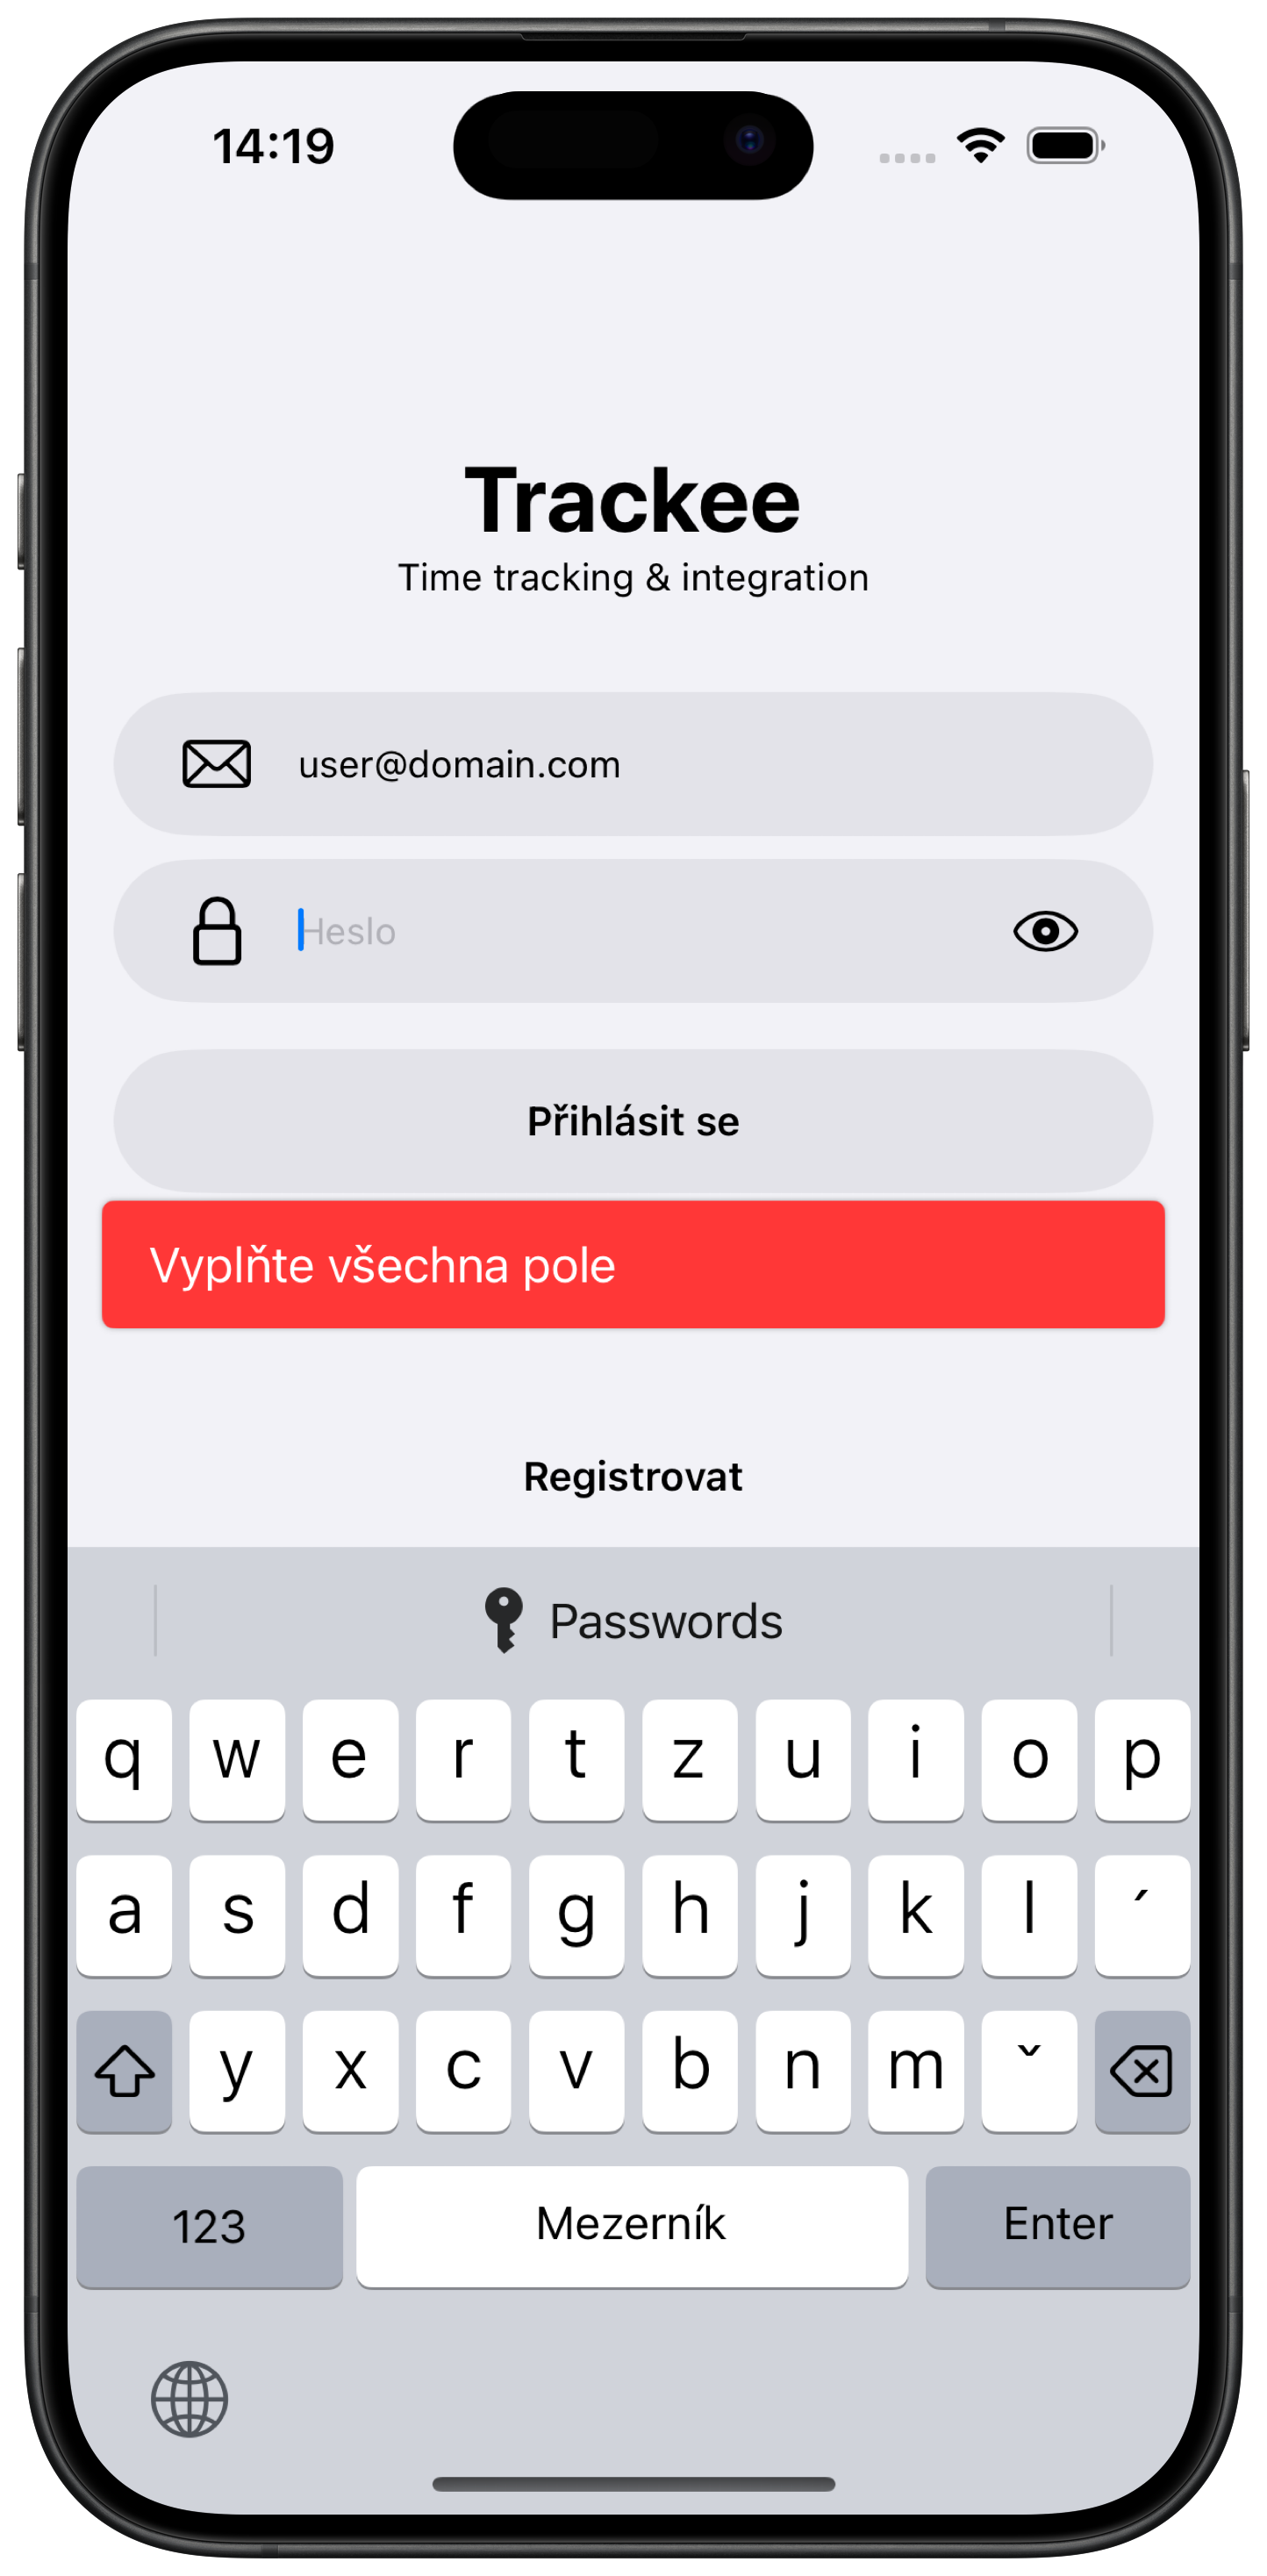
\includegraphics[width=6cm]{login-error-impl.png}
		\caption{Chyba při přihlášení}
		\label{fig:login-error-impl}
	\end{subfigure}
	\hspace{2cm}
	\begin{subfigure}[b]{0.4\textwidth}
		\centering
		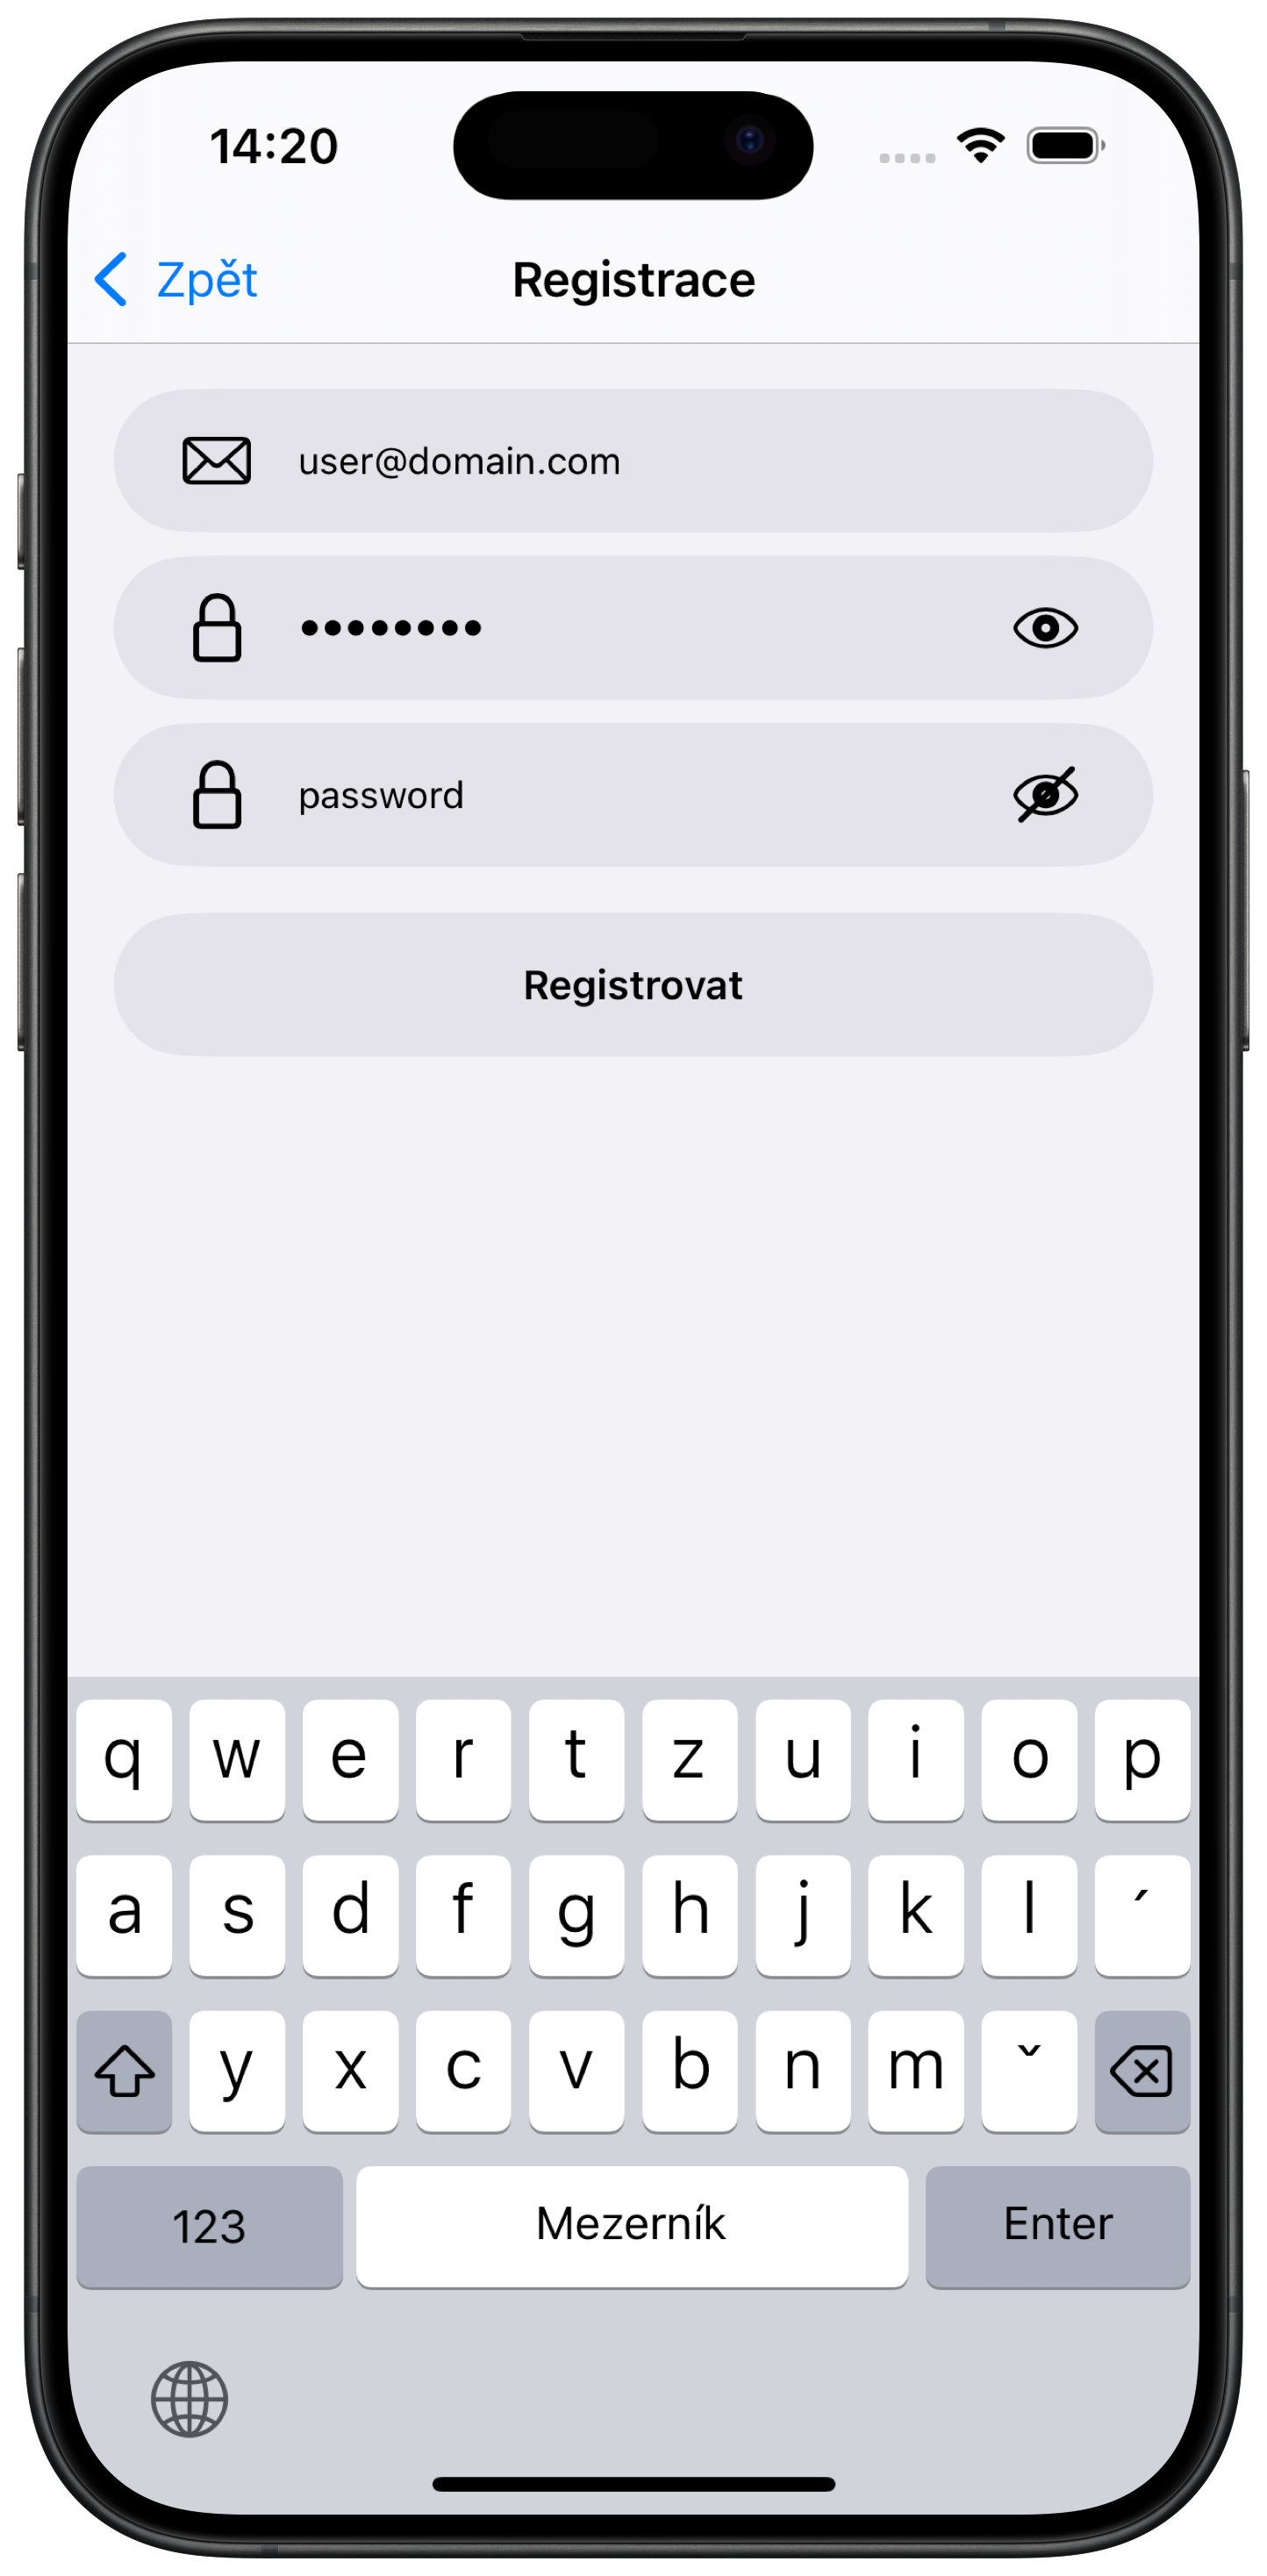
\includegraphics[width=6cm]{register-impl.png}
		\caption{Registrace}
	\end{subfigure}
	\caption{Realizace přihlášení a~registrace}
	\label{fig:onboarding-impl}
\end{figure}

%---------------------------------------------------------------
\subsection{Časovač}
%---------------------------------------------------------------

Tato funkcionalita pokrývá veškeré operace s~ovládáním časovače, získáváním historie časových záznamů a~vytváření nových záznamů. Jedná se o~hlavní funkci aplikace.

%---------------------------------------------------------------
\subsubsection{Backend}
%---------------------------------------------------------------

Backendová část platformy bude muset spravovat veškerá data, která se týkají časovače a~časových záznamů. Backend je ale rozdělený podle funkcionalit jiným způsobem, než nativní aplikace a~multi-platformní část, které jsou rozděleny podle funkcionalit z~hlediska uživatele. Moduly backendu jsou rozděleny podle toho, čeho se data v~modulu týkají, tedy například klienti, projekty, integrace a~uživatel. Jelikož pro data časovače budou potřeba data uživatele, u~kterého se ukládá aktuální nastavení časovače a~historie časových záznamů, ale také data projektů a~klientů, bude implementace funkcionality časovače zasahovat do více modulů. Největší část funkcionality časovače bude obsluhovat modul uživatele. 

Obrazovka časovače bude potřebovat následující data – souhrn odpracovaných hodin v~aktuální den a~týden, historii časových záznamů, aktuální nastavení časovače a~přehled projektů, bude-li si uživatel chtít vybrat projekt, který časovači přidělí.

V~první řadě je tedy potřeba implementovat získávání historie časových záznamů, protože to bude potřeba i~pro výpočet odpracovaných hodin v~aktuálním dnu a~týdnu. V~návrhu v~sekci \ref{feature-timer} bylo popsáno, že načítání historie časových záznamů by mělo podporovat stránkování, jelikož může teoreticky obsahovat velké množství záznamů, a~pokud by se mělo velké množství načítat celé najednou, mohlo by to trvat dlouho a~mohlo by se jednat o~velké množství dat, která by ale uživatel nejspíš ani všechna vůbec nepotřeboval. \texttt{UserRepository} tedy definuje mimo jiné funkce pro získávání záznamů, které lze nahlédnout v~ukázce kódu \ref{code:be-read-entries-interface}. Tyto funkce potřebují parametr \texttt{uid} identifikující uživatele, pro kterého mají být záznamy čteny, a~dále přijímají nepovinné parametry pro specifikaci toho, od kdy a~do kdy mají být záznamy čteny, a~kolik maximálně záznamů se ve stránce má nacházet. Pokud bude mít některý z~těchto nepovinných parametrů hodnotu \texttt{null}, nebude žádné omezení na záznamy klást. Rozdíl mezi funkcemi, které vrací stránky objektu \texttt{TimerEntry} a~stránky objektu \texttt{TimerEntryPreview} je ten, že objekt \texttt{TimerEntryPreview} obsahuje navíc celé zdrojové objekty klienta a~projektu, který k~záznamu patří, zatímco \texttt{TimerEntry} obsahuje pouze jejich identifikátory. V~obrazovce pro zobrazení historie záznamů budou tyto zdrojové objekty potřeba, protože při jejich vizualizaci (při jejich \emph{preview}) bude potřeba zobrazit jméno klienta a~projektu.

\begin{listing}
\caption{Funkce pro získávání časových záznamů v~\texttt{UserRepository}}\label{code:be-read-entries-interface}
\begin{minted}{Kotlin}
interface UserRepository {

    // ...
    
    suspend fun readEntries(
        uid: String,
        startAfter: Instant?,
        limit: Int?,
        endAt: Instant?
    ): Page<TimerEntry>
    
    // ...
    
    suspend fun readEntryPreviews(
        uid: String,
        startAfter: Instant?,
        limit: Int?,
        endAt: Instant?
    ): Page<TimerEntryPreview>
    
    // ...
}
\end{minted}
\end{listing}

V~ukázce kódu \ref{code:be-read-entries-source} lze poté vidět, jakým způsobem aplikace získává záznamy přímo z~\emph{Firestore} databáze. Omezení ve smyslu od kdy do kdy záznamy číst a~kolik maximálně jich přečíst se implementuje pomocí funkcí \texttt{startAfter(start)}, \texttt{endAt(end)} a~\texttt{limit(limit)}, které přímo nabízí \emph{Firestore} API. \texttt{UserRepositoryImpl} používá tuto \emph{Source} funkci i~pro načtení \emph{preview} objektů, objekty klienta a~projektu si pak pomocí identifikátoru načte sama a~připojí je.

\begin{listing}
\caption{Funkce pro získávání časových záznamů v~\texttt{UserSourceImpl}}\label{code:be-read-entries-source}
\begin{minted}{Kotlin}
internal class UserSourceImpl : UserSource {

    // ...
    
    override suspend fun readEntries(
        uid: String,
        startAfter: Instant?,
        limit: Int?,
        endAt: Instant?
    ): Page<FirestoreTimerEntry> {
        val entriesCollection = db
            .collection(SourceConstants.Firestore.Collection.ENTRIES)
            .document(uid)
            .collection(SourceConstants.Firestore.Collection.ENTRIES)
            .orderBy(
                SourceConstants.Firestore.FieldName.STARTED_AT, 
                Query.Direction.DESCENDING
            )

        val snapshot = entriesCollection
            .startAfter(startAfter?.toTimestamp() ?: Timestamp.now())
            .endAt(endAt?.toTimestamp() ?: Timestamp.MIN_VALUE)
            .limit(limit ?: Int.MAX_VALUE)
            .get()
            .await()

        val data = snapshot.documents.map { 
            it.toObject(FirestoreTimerEntry::class.java) 
        }

        val remainingCount = entriesCollection
            .startAfter(data.lastOrNull()?.startedAt ?: Timestamp.MIN_VALUE)
            .count()
            .get()
            .await()
            .count

        return Page(
            data = data,
            isLast = remainingCount == 0.toLong()
        )
    }
    
    // ...
}
\end{minted}
\end{listing}

Při načítání historie záznamů na obrazovce časovače pak bude potřeba použít parametry \texttt{startAfter}, abychom definovali datum a~čas, od kterého další záznamy načítat, pokud načítáme další stránky, a~\texttt{limit}, který určí velikost stránky. Při načítání všech záznamů v~daném období se pak využije parametrů \texttt{startAfter} a~\texttt{endAt}, například když bude potřeba zjistit souhrn odpracovaných hodin v~aktuální den nebo týden. Při výpočtu tohoto souhrnu bude tedy \texttt{UserRepositoryImpl} sčítat doby trvání všech záznamů v~daném období.

Pro obsluhu časovače pak \texttt{UserRepository} poskytuje funkce pro načtení dat časovače a~pro jejich aktualizaci. Při výběru projektu bude uživatel potřebovat vidět všechny své projekty a~názvy jejich klientů, pro což bude sloužit opět \emph{preview} objekt \texttt{ProjectPreview}. \texttt{ClientRepository} tedy nabízí funkce pro získání klienta podle identifikátoru, a~\texttt{UserRepository} nabízí funkce pro získání projektu podle identifikátoru klienta a~projektu, ale také funkci pro získání všech projektů daného uživatele.

Pro komunikaci s~klientem se také využívá vlastních struktur pro reprezentaci chyb. Například modul \texttt{user} používá výjimky ze skupiny \texttt{UserExceptions}, která dědí z~třídy \texttt{BaseException}. V~případě, že některé volání vrátí výjimku s~tímto rodičem, tak ji komunikace umí zakódovat do DTO reprezentace, která je známá pro klienta. Ten může potom rozlišovat mezi různými známými chybami. V~případě, že se nejedná o~známou chybu, zakóduje ji komunikace jako obecnou chybu s~HTTP status kódem 500. Implementace tohoto chování lze nahlédnout ve výpisu kódu \ref{code:be-error-handling}.

\begin{listing}
\caption{Obsluha chyb na backendu}\label{code:be-error-handling}
\begin{minted}{Kotlin}
fun Application.configureRouting(isDebug: Boolean) {
    install(StatusPages) {
        exception<BaseException> { call, baseException ->
            call.respond(
                status = baseException.code,
                baseException.toDto(isDebug)
            )
        }

        exception<Throwable> { call, cause ->
            call.respond(
                status = HttpStatusCode.InternalServerError,
                message = ErrorDto(
                    type = "InternalError",
                    message = "Internal Server Error",
                    debugMessage = if (isDebug) cause.message else null
                )
            )
        }
    }
    
    // ...
}
\end{minted}
\end{listing}

%---------------------------------------------------------------
\subsubsection{Multi-platformní část}
%---------------------------------------------------------------

Multi-platformní část aplikace už rozděluje své moduly podle funkcionalit z~hlediska uživatele, modul \texttt{timer} bude tedy poskytovat všechny \emph{Use Cases} pro potřeby časovače:
\begin{itemize}
\item\texttt{AddTimerEntryUseCase} – Vytvoří nový časový záznam podle parametrů.
\item\texttt{DeleteTimerEntryUseCase} – Smaže časový záznam podle identifikátoru.
\item\texttt{GetProjectsUseCase} – Získá \emph{preview} objekty všech projektů, které má uživatel přiřazeny.
\item\texttt{GetTimerDataPreviewUseCase} – Získá \emph{preview} objekt pro aktuální nastavení časovače. Čistá data o~aktuálním stavu časovače totiž opět obsahují jen identifikátory klienta a~projektu, ale při vizualizaci dat jsou potřeba jejich názvy.
\item\texttt{GetTimerEntriesUseCase} – Získává stránky \emph{preview} objektů časových záznamů, umí tedy pracovat se všemi parametry pro omezení stránky. Zároveň časové záznamy seskupuje do seznamu objektů typu \texttt{TimerEntryGroup}, což je skupina, která obsahuje datum, seznam všech záznamů patřící k~tomuto datu a~součet odpracovaných hodin všech těchto záznamů. Toho se využije při vizualizaci v~nativní aplikaci, kde se nad každou skupinou ukáže datum a~časový souhrn pro daný den.
\item\texttt{GetTimerSummariesUseCase} – Získá souhrny časových záznamů pro aktuální den a~týden.
\item\texttt{UpdateTimerDataUseCase} – Aktualizuje aktuální nastavení časovače.
\end{itemize}

Všechny tyto \emph{Use Cases} automaticky počítají s~tím, že pracují s~daty aktuálně přihlášeného uživatele, žádné parametry pro jeho identifikaci tedy nepotřebují.

Jednotlivé \emph{Use Cases} už komunikují s~backendem, a~to v~nejnižší \emph{infrastructure} vrstvě, která požadavky posílá pomocí knihovny \emph{Ktor}. Příklad toho, jak probíhá komunikace, lze nahlédnout v~ukázce kódu \ref{code:kmp-read-entries-source-impl}.

\begin{listing}
\caption{Funkce pro získávání časových záznamů v~\texttt{RemoteTimerSource}}\label{code:kmp-read-entries-source-impl}
\begin{minted}{Kotlin}
internal class RemoteTimerSource(
    private val client: HttpClient
) : TimerSource {
    override suspend fun readEntries(
        startAfter: String?,
        limit: Int?,
        endAt: String?
    ): Result<PageDto<TimerEntryDto>> =
        runCatchingCommonNetworkExceptions {
            val res = client.get("user/entries") {
                url {
                    startAfter?.let { parameters.append("startAfter", it) }
                    limit?.let { parameters.append("limit", it.toString()) }
                    endAt?.let { parameters.append("endAt", it) }
                }
            }
            res.body<PageDto<TimerEntryDto>>()
        }
        
    // ...
}
\end{minted}
\end{listing}

Multi-platformní část pracuje s~objekty v~DTO reprezentaci, kterou definuje backend. Poté si je také převádí pomocí vlastních funkcí do vlastních doménových reprezentací.

Také lze ve výpisu kódu \ref{code:kmp-read-entries-source-impl} nahlédnout, že celé API volání je obaleno do pomocné funkce \texttt{runCatchingCommonNetworkExceptions}, jejíž implementace lze nahlédnout ve výpisu \ref{code:kmp-run-catching-common-network-exceptions}. Tato funkce odchytává všechny výjimky, které při komunikaci s~backendem mohou vzniknout, a~převádí je do vlastních reprezentací, se kterými poté umí pracovat nativní aplikace.

\begin{listing}
\caption{Odchytávání výjimek při komunikaci s~backendem}\label{code:kmp-run-catching-common-network-exceptions}
\begin{minted}{Kotlin}
internal suspend inline fun <R : Any> runCatchingCommonNetworkExceptions(
    block: () -> R
): Result<R> =
    try {
        Result.Success(block())
    } catch (e: ResponseException) {
        val body = e.response.body<ErrorDto>()

        val error = when (body.type) {
            "Unauthorized" -> BackendError.NotAuthorized(e.response.toString(), e)
            "ProjectNotAssignedToUser" -> BackendError.ProjectNotAssignedToUser(
                body.message,
                e
            )
            "MissingProject" -> BackendError.MissingProject(body.message, e)
            "ProjectNotFound" -> BackendError.ProjectNotFound(body.message, e)
            "ClientNotFound" -> BackendError.ClientNotFound(body.message, e)
            "ClockifyProjectNotFound" -> BackendError.ClockifyProjectNotFound(
                body.message, 
                e
            )
            "ClockifyInvalidApiKey" -> BackendError.ClockifyInvalidApiKey(e)
            "ClockifyUnknownError" -> BackendError.ClockifyUnknownError(e)
            "ClockifyWorkspaceNotFound" -> BackendError.ClockifyWorkspaceNotFound(
                body.message,
                e
            )
            else -> ErrorResult(message = body.message, throwable = e)
        }

        Result.Error(error)
    } catch (e: Throwable) {
        val error = when (e::class.simpleName) {
            "UnknownHostException" -> CommonError.NoNetworkConnection(e)
            "HttpRequestTimeoutException", "ConnectTimeoutException",
            "SocketTimeoutException" -> CommonError.Timeout(e)
            "CancellationException" -> CommonError.Cancelled(e)
            else -> handlePlatformError(e)
        }
        Result.Error(error)
    }
\end{minted}
\end{listing}

%---------------------------------------------------------------
\subsubsection{Nativní aplikace}
%---------------------------------------------------------------

Realizace časovače dodržuje vzhled navržený v~sekci \ref{feature-timer}. Na obrázku \ref{fig:timer-empty-impl} lze nahlédnout obrazovka časovače, jak bude vypadat, pokud uživatel zatím nemá žádná data, jako například nově registrovaný uživatel. Na obrázku \ref{fig:fetch-more-impl} lze zase nahlédnout, jak vypadá tlačítko pro načtení dalších záznamů, pokud se uživatel posune v~načtených datech úplně nahoru. Na obrázku \ref{fig:description-edit-impl} lze nahlédnout stav, kdy si uživatel chce změnit popisek časovače, a~na obrázku \ref{fig:time-selection-impl} zase obrazovka pro ruční vybrání času, pokud chce uživatel přidat záznam manuálně. Na obrázku \ref{fig:project-selection-impl} lze poté vidět výběr z~projektů a~možnost v~nich vyhledávat.

\begin{figure}[p]
    \centering
    \begin{subfigure}[b]{0.4\textwidth}
		\centering
		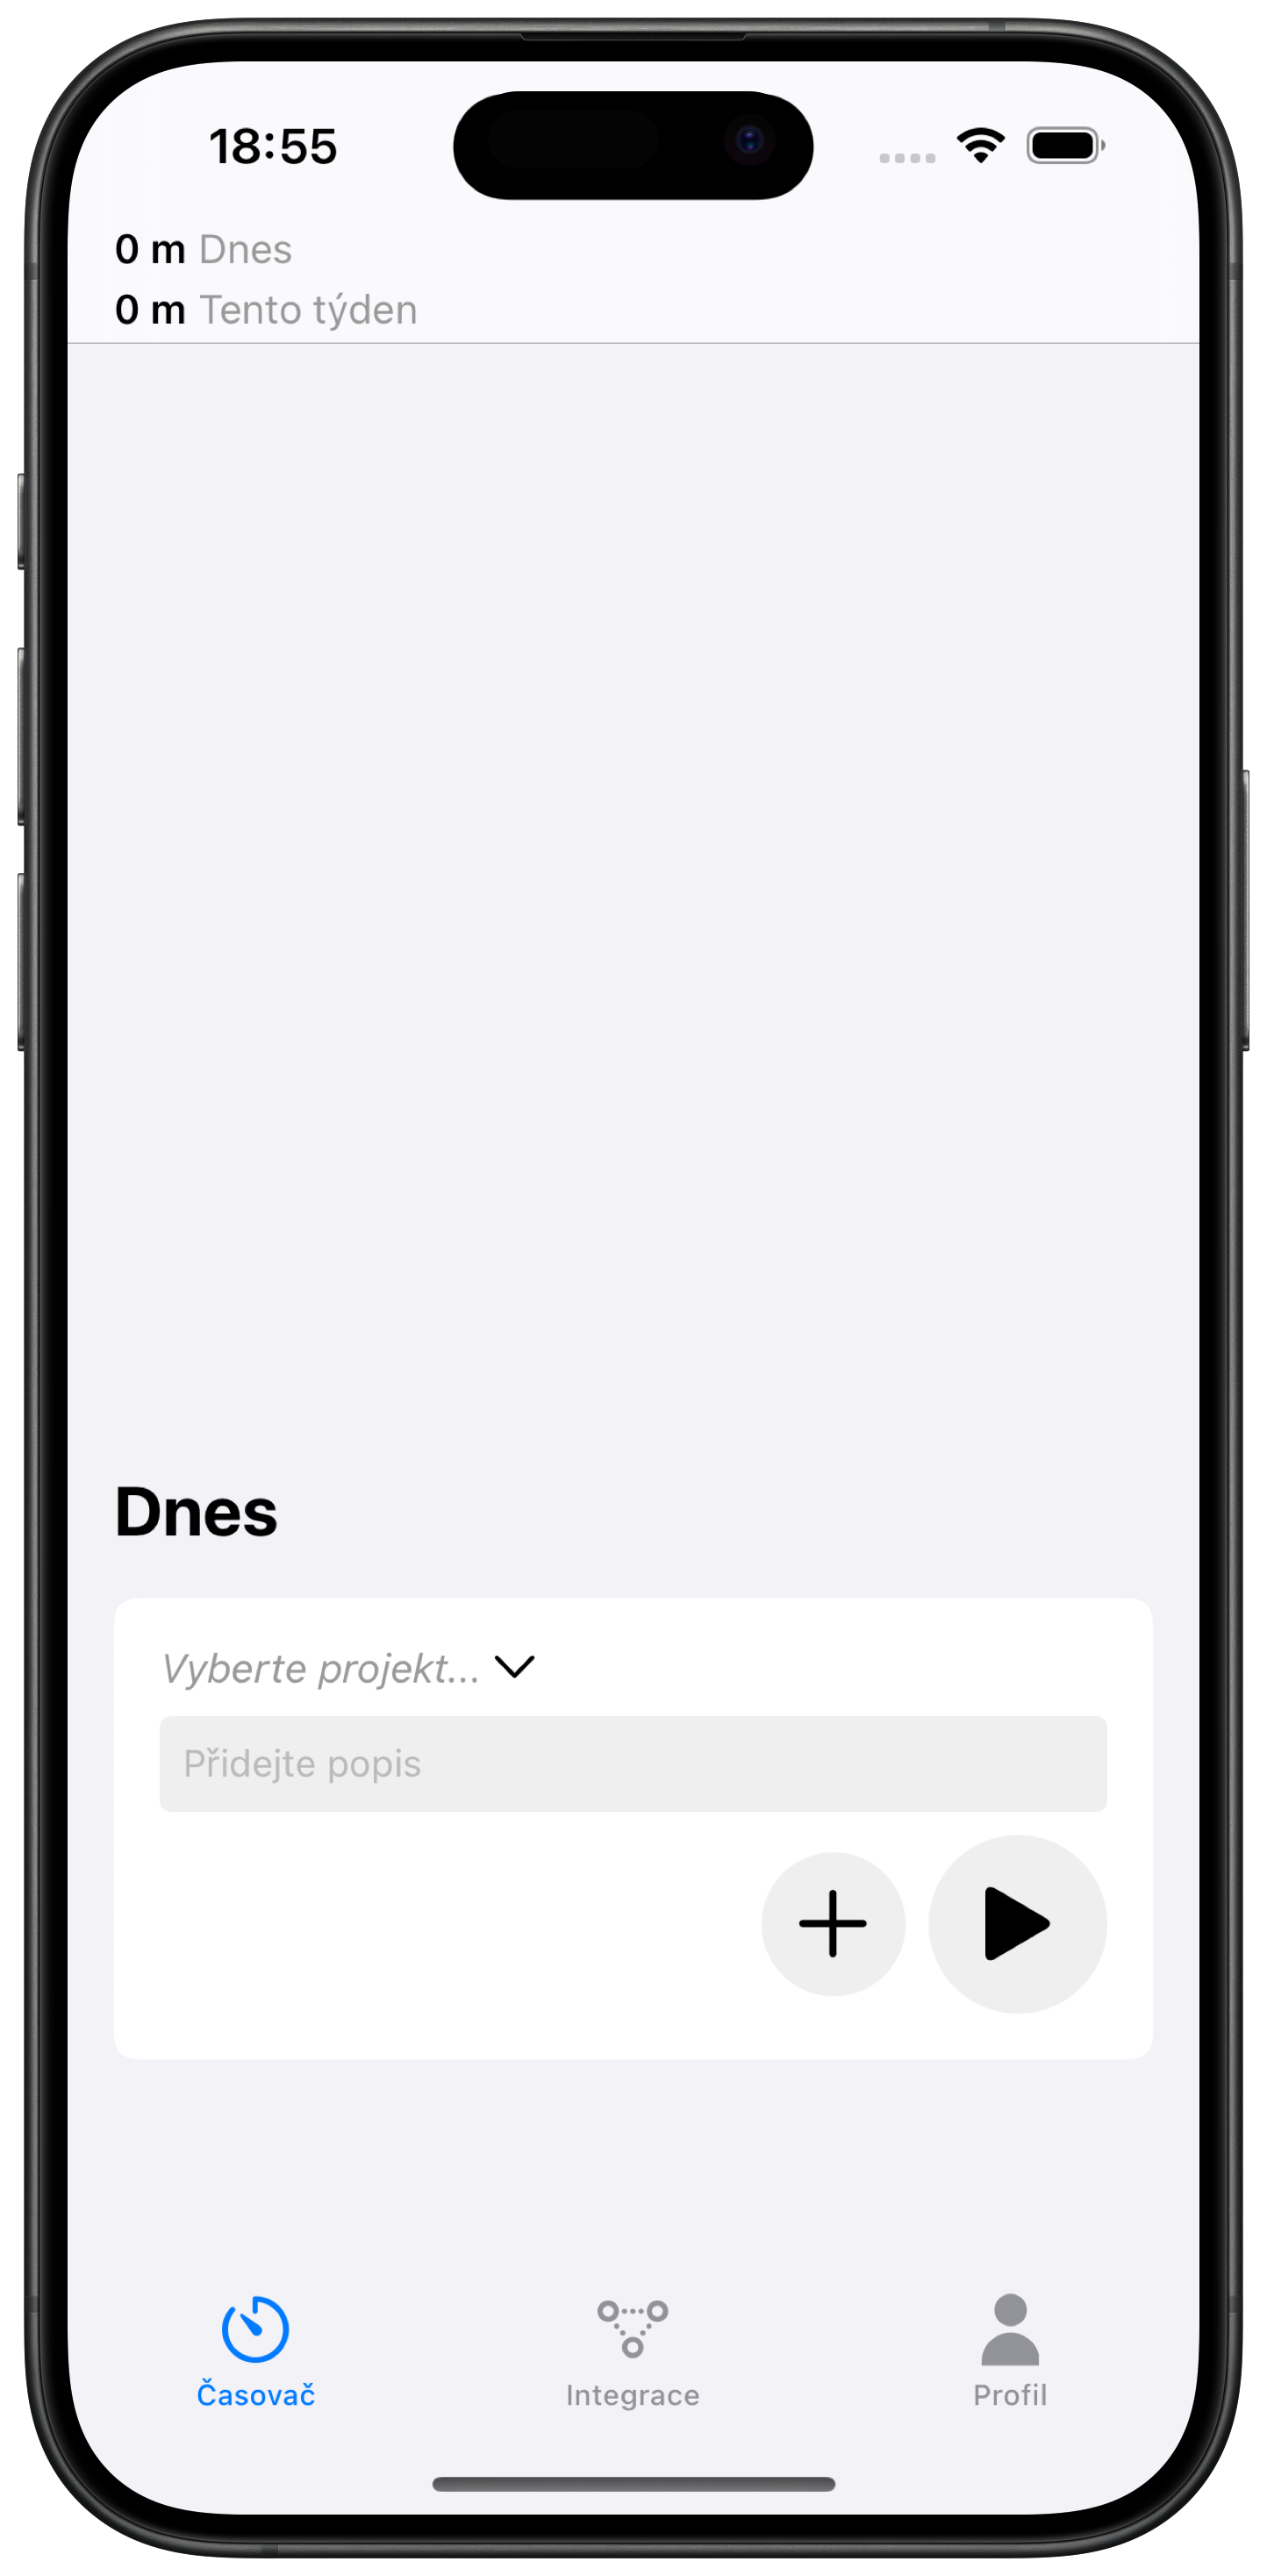
\includegraphics[width=6cm]{timer-empty-impl.png}
		\caption{Prázdná data}
		\label{fig:timer-empty-impl}
	\end{subfigure}
	\hspace{2cm}
	\begin{subfigure}[b]{0.4\textwidth}
		\centering
		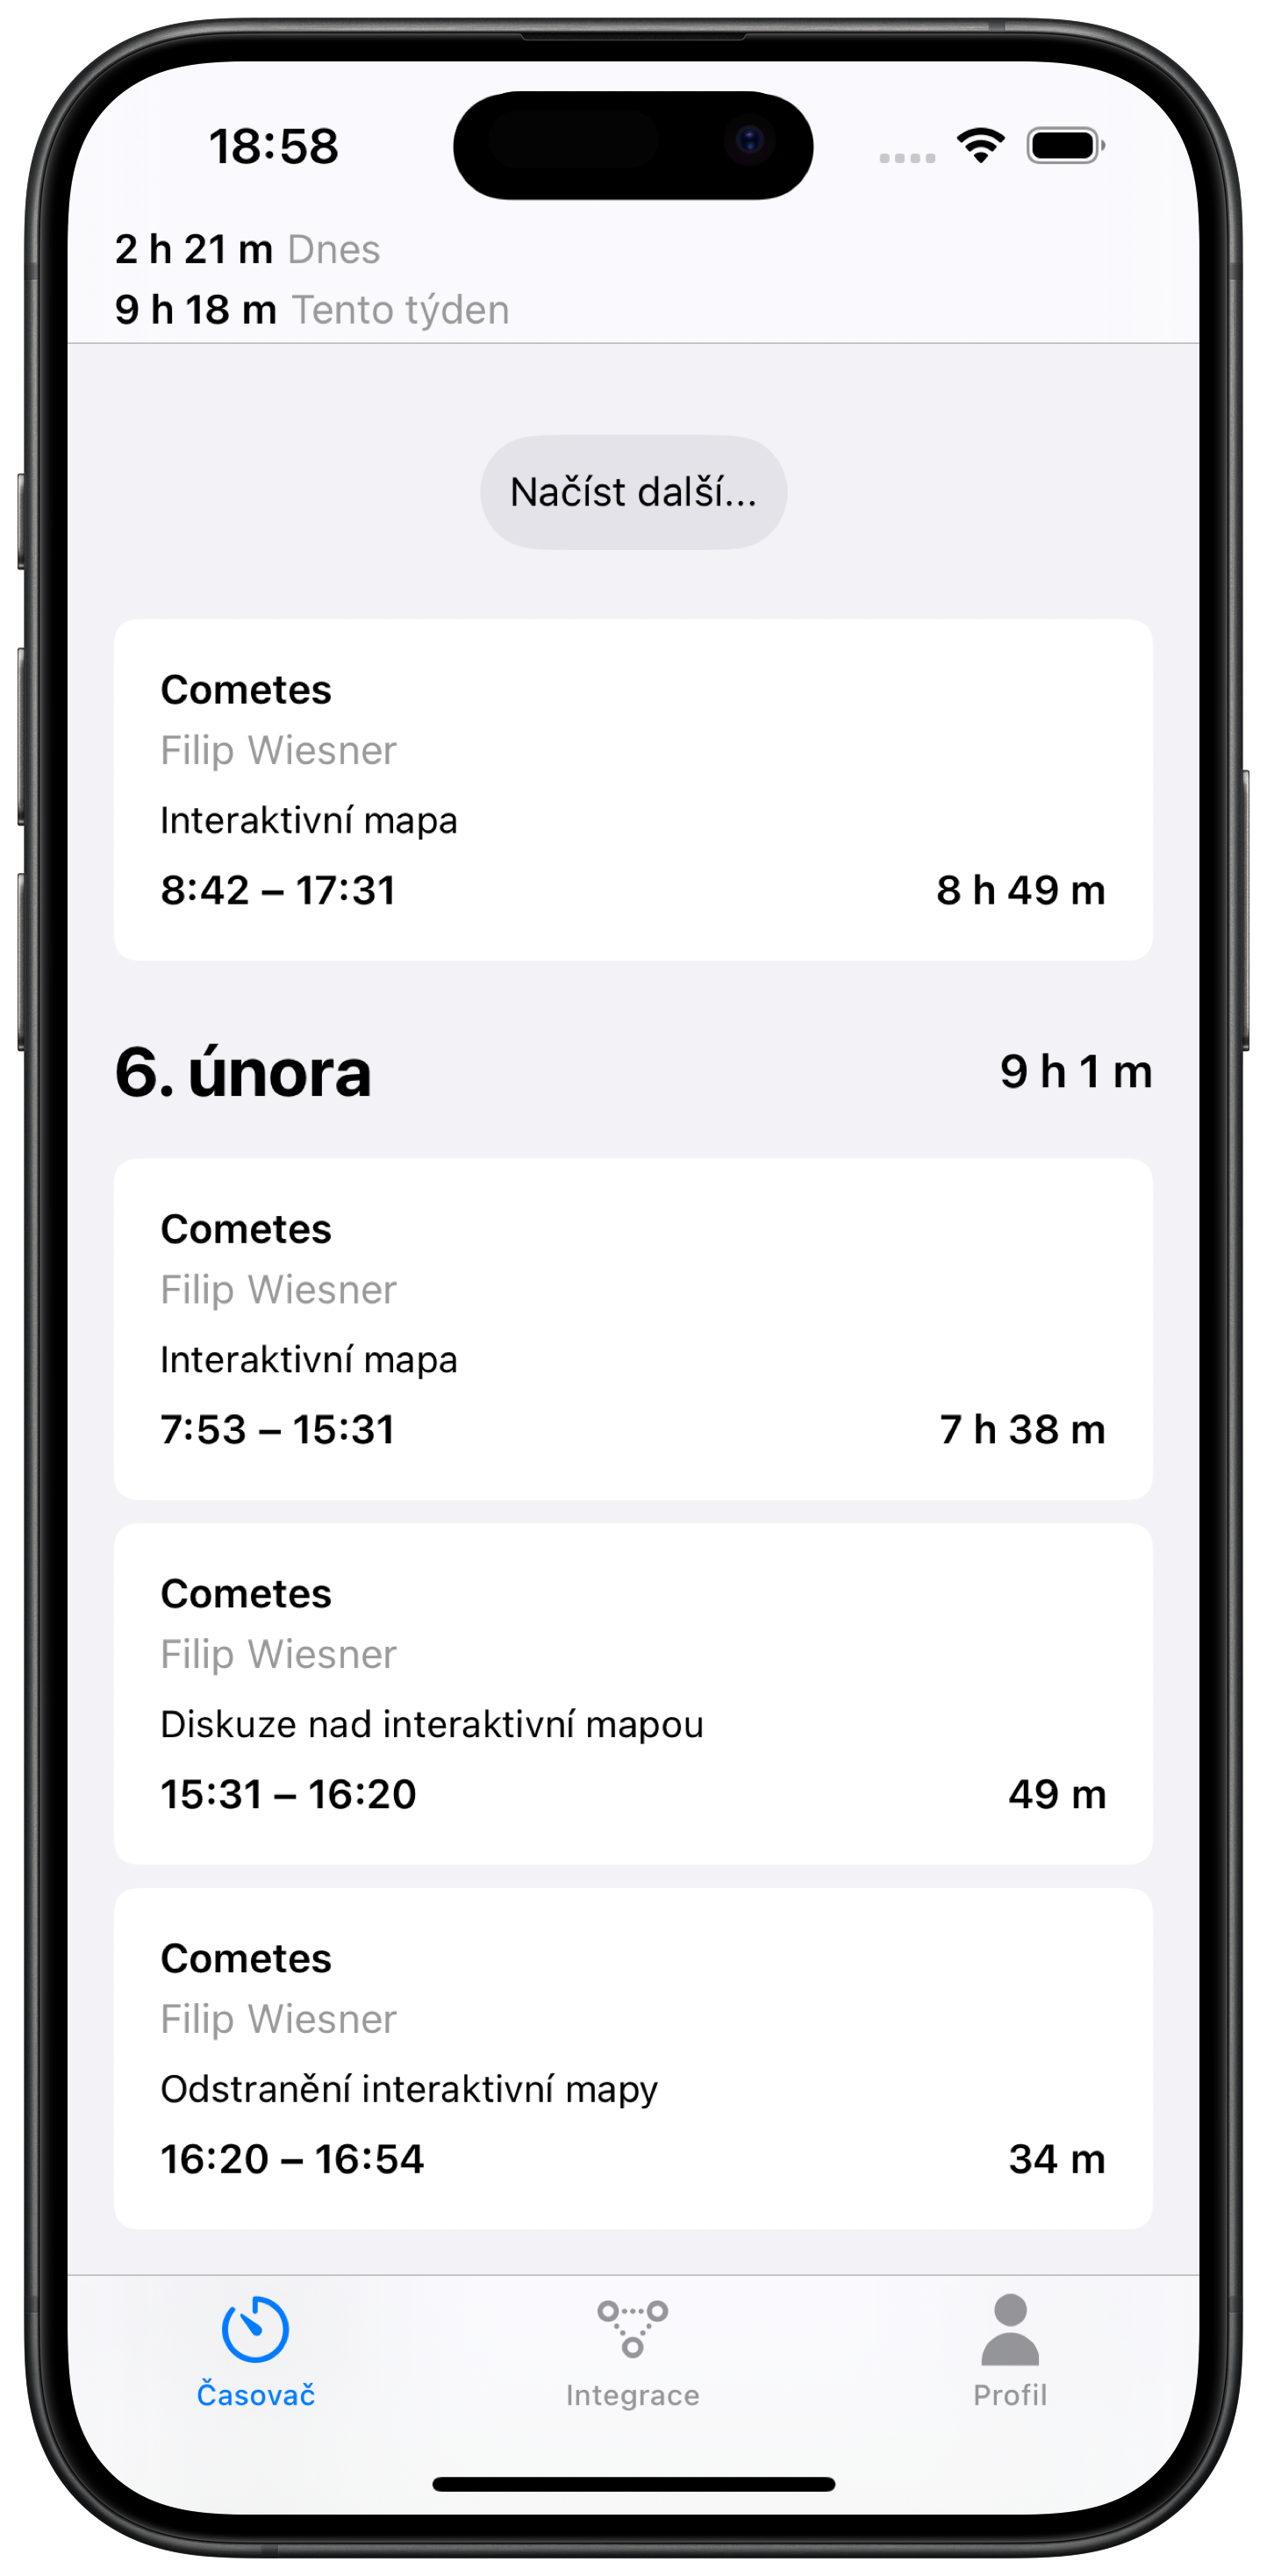
\includegraphics[width=6cm]{fetch-more-impl.png}
		\caption{Načtení další stránky}
		\label{fig:fetch-more-impl}
	\end{subfigure}
	\caption{Realizace časovače}
	\label{fig:timer-impl}
\end{figure}

\begin{figure}[p]
    \centering
    \begin{subfigure}[b]{0.4\textwidth}
		\centering
		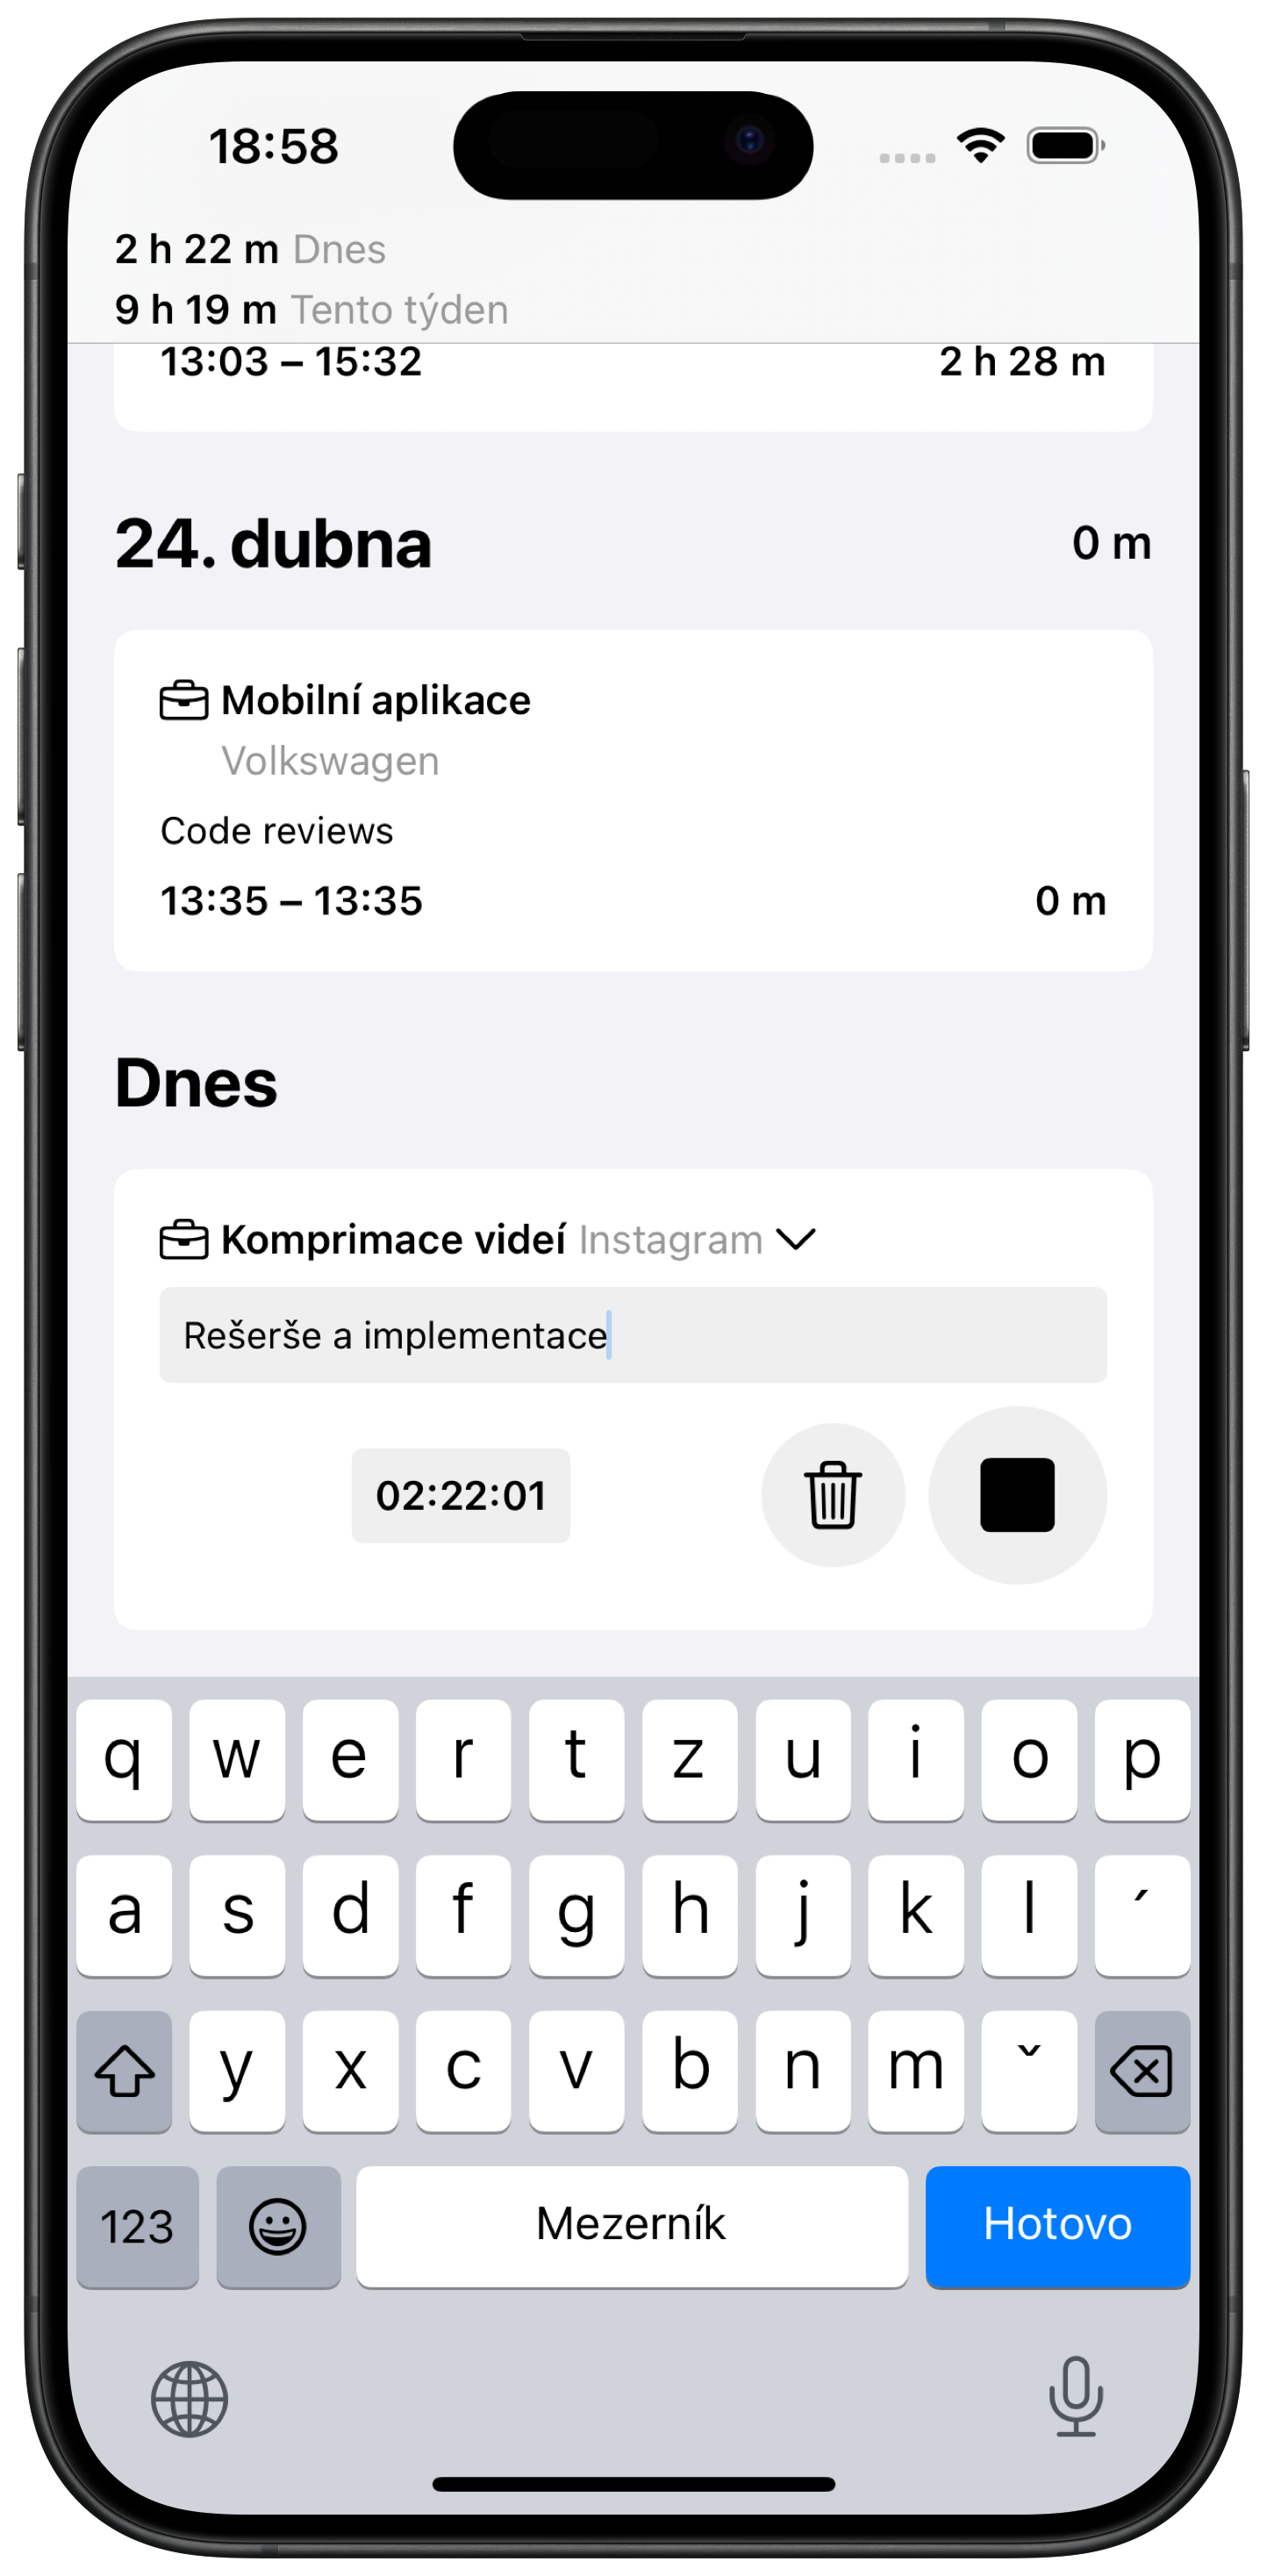
\includegraphics[width=6cm]{description-edit-impl.png}
		\caption{Úprava popisu}
		\label{fig:description-edit-impl}
	\end{subfigure}
	\hspace{2cm}
	\begin{subfigure}[b]{0.4\textwidth}
		\centering
		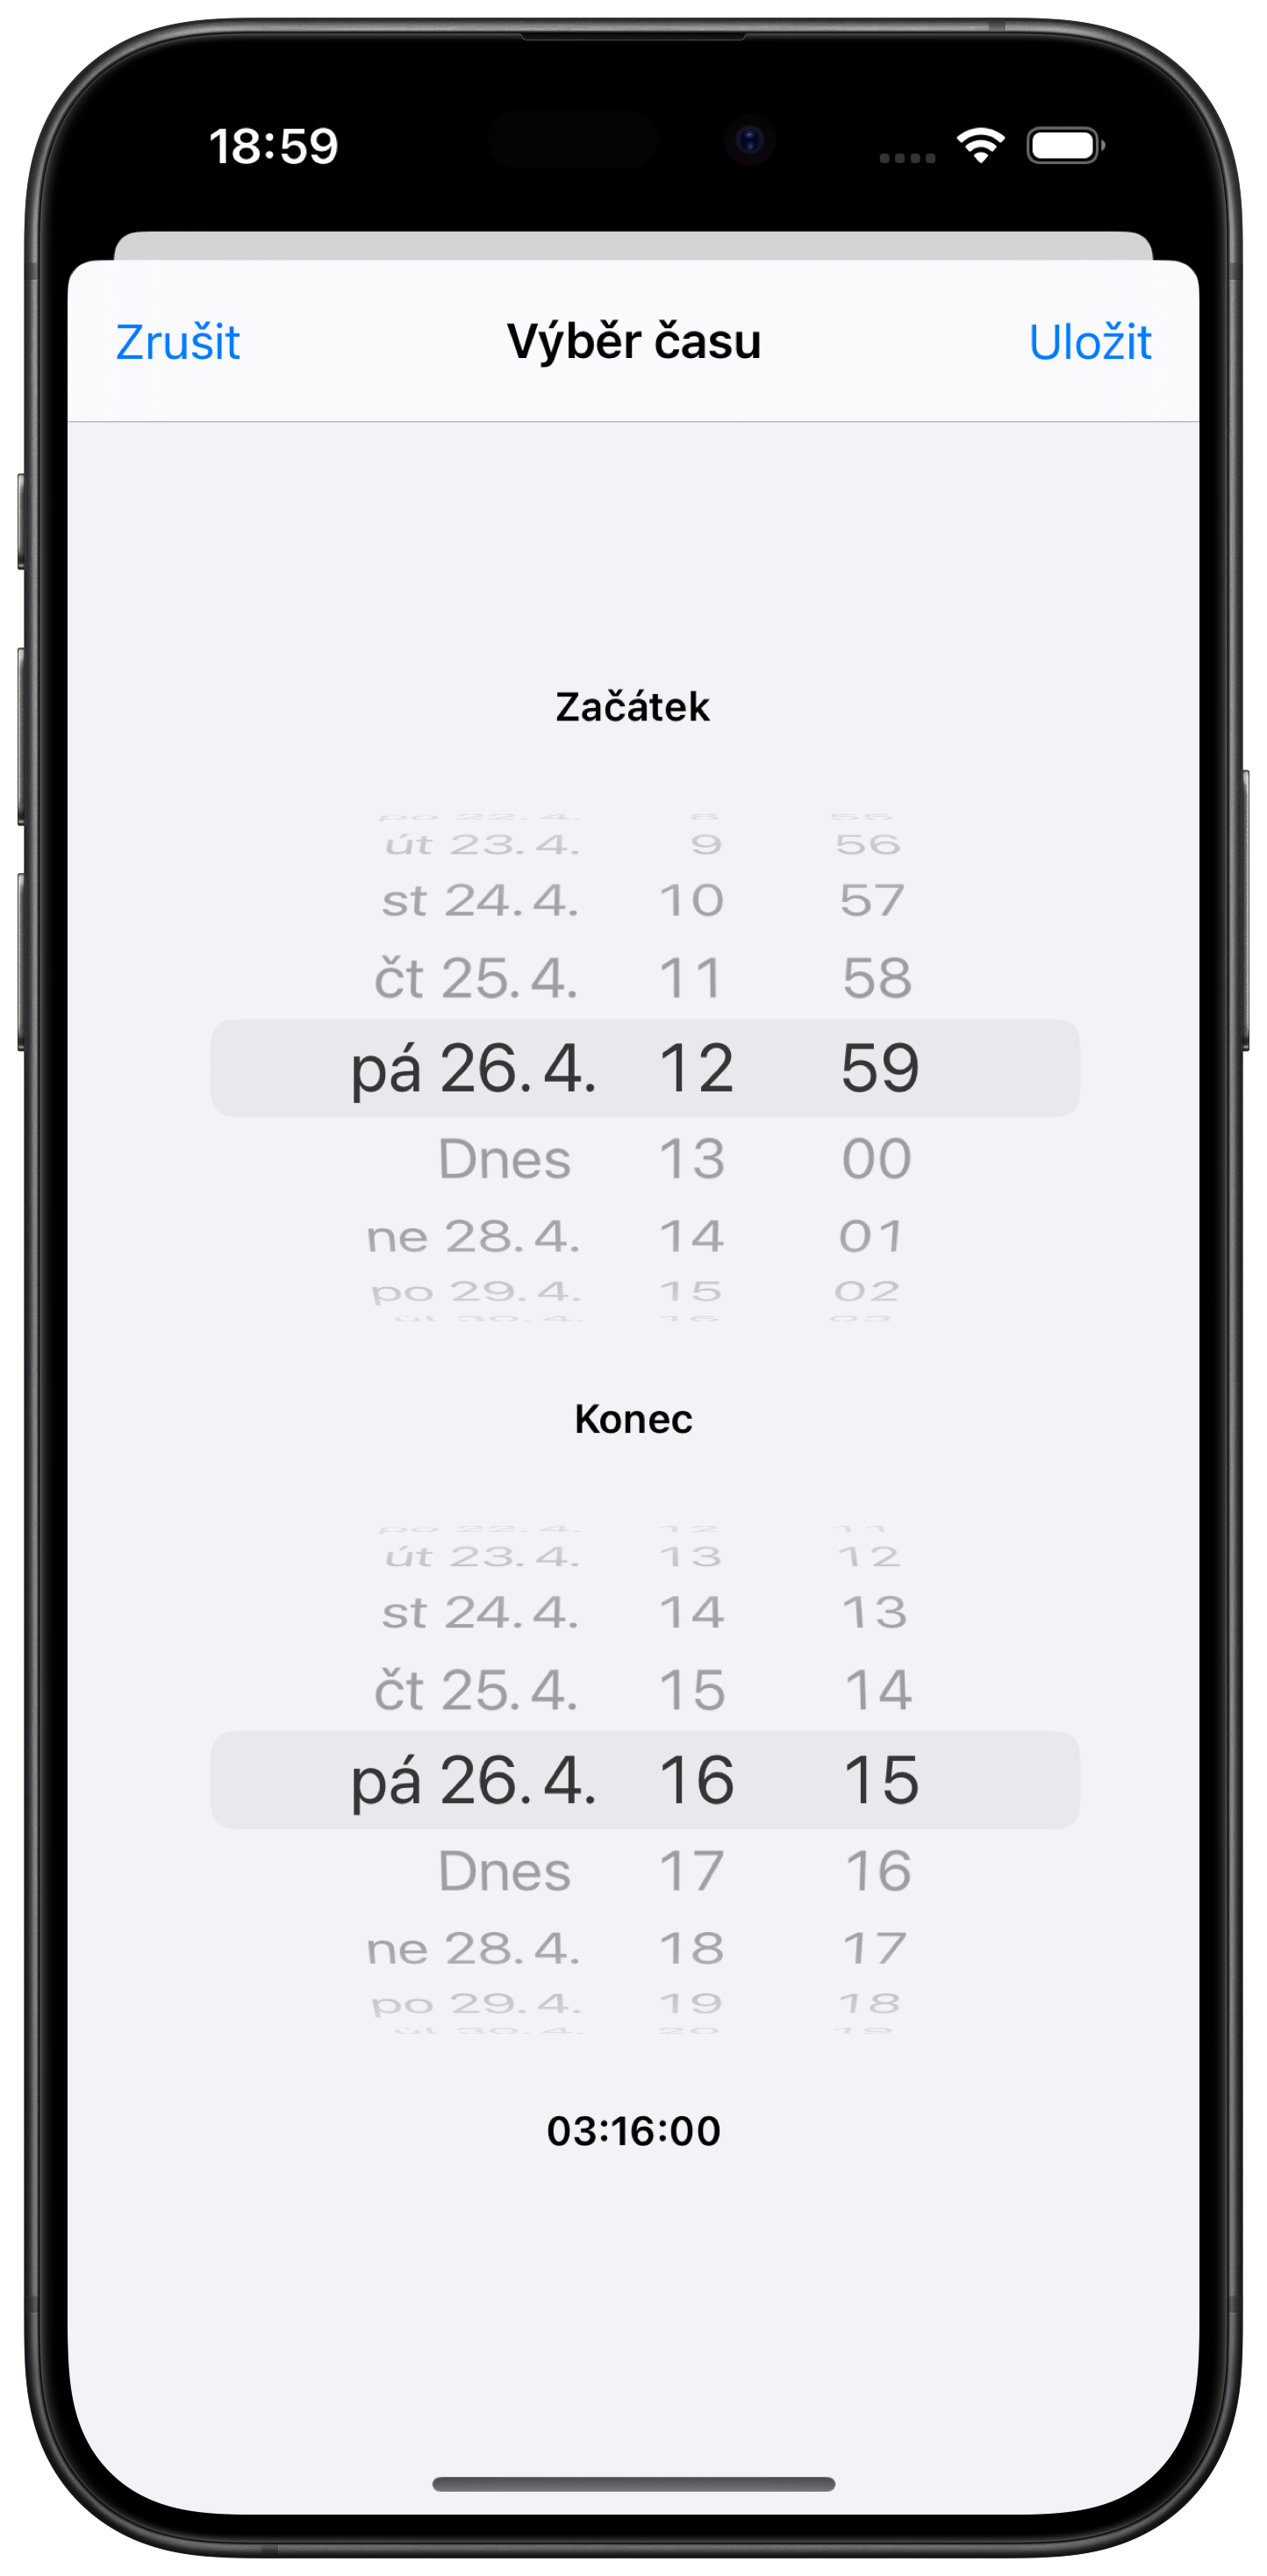
\includegraphics[width=6cm]{time-selection-impl.png}
		\caption{Manuální výběr času}
		\label{fig:time-selection-impl}
	\end{subfigure}
	\caption{Realizace ovládání časovače}
	\label{fig:timer-control-impl}
\end{figure}

\begin{figure}[p]
    \centering
    \begin{subfigure}[b]{0.4\textwidth}
		\centering
		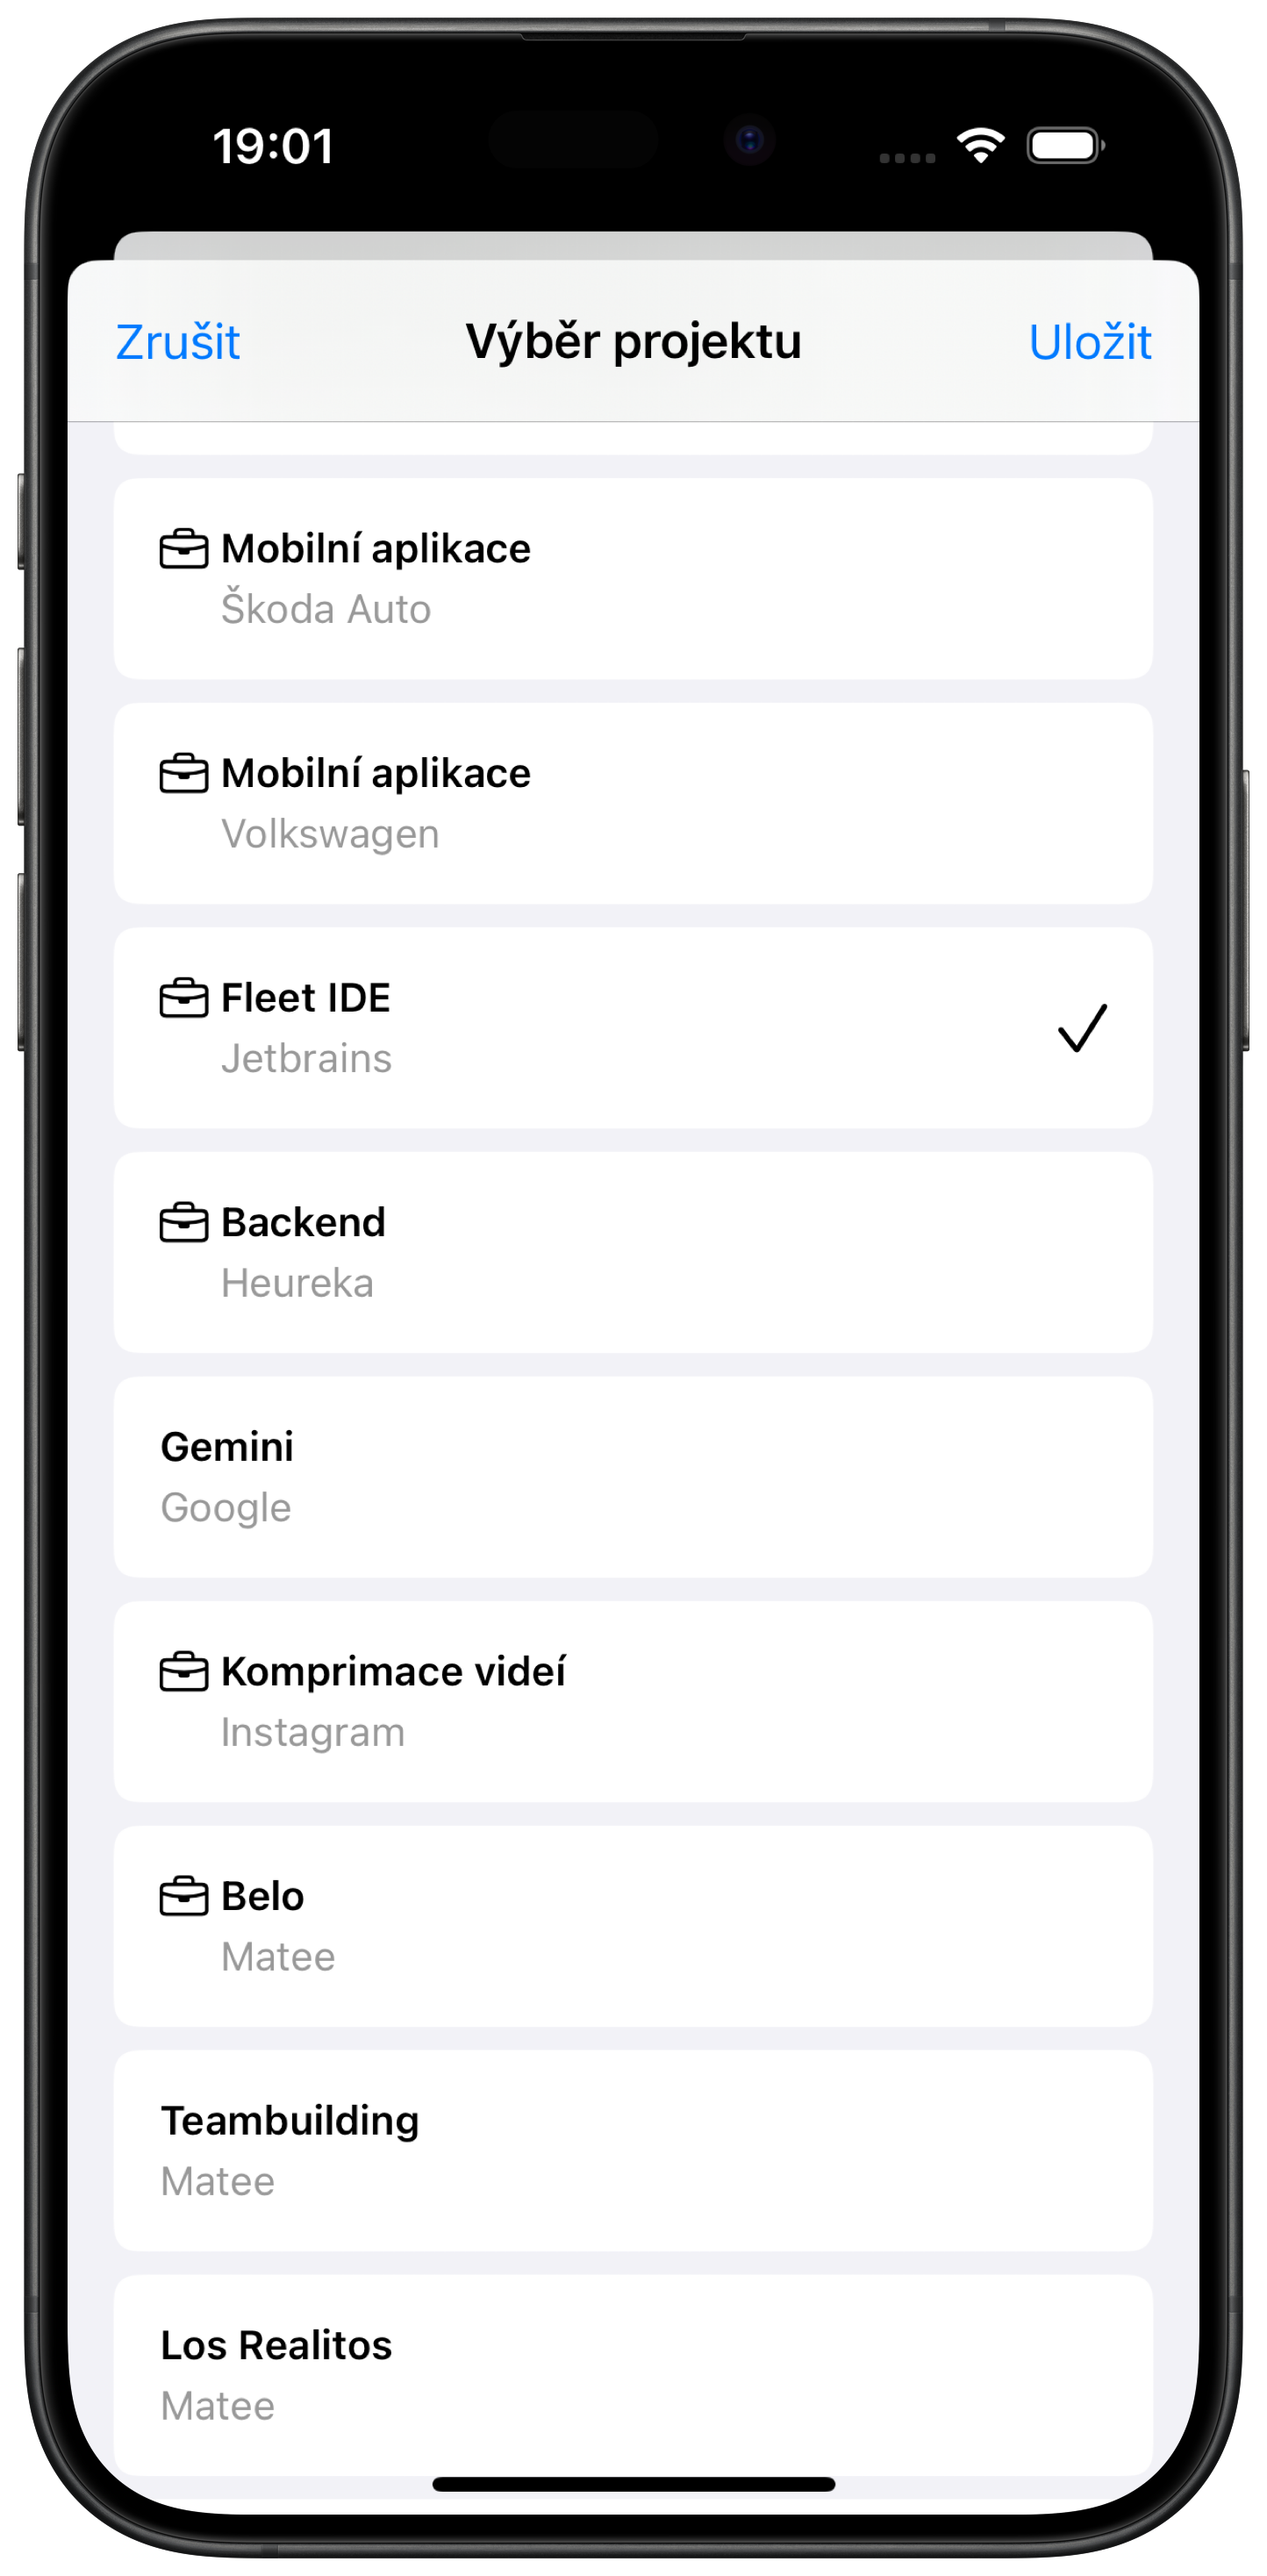
\includegraphics[width=6cm]{project-selection-impl.png}
		\caption{Vybraný projekt}
		\label{fig:selected-project-impl}
	\end{subfigure}
	\hspace{2cm}
	\begin{subfigure}[b]{0.4\textwidth}
		\centering
		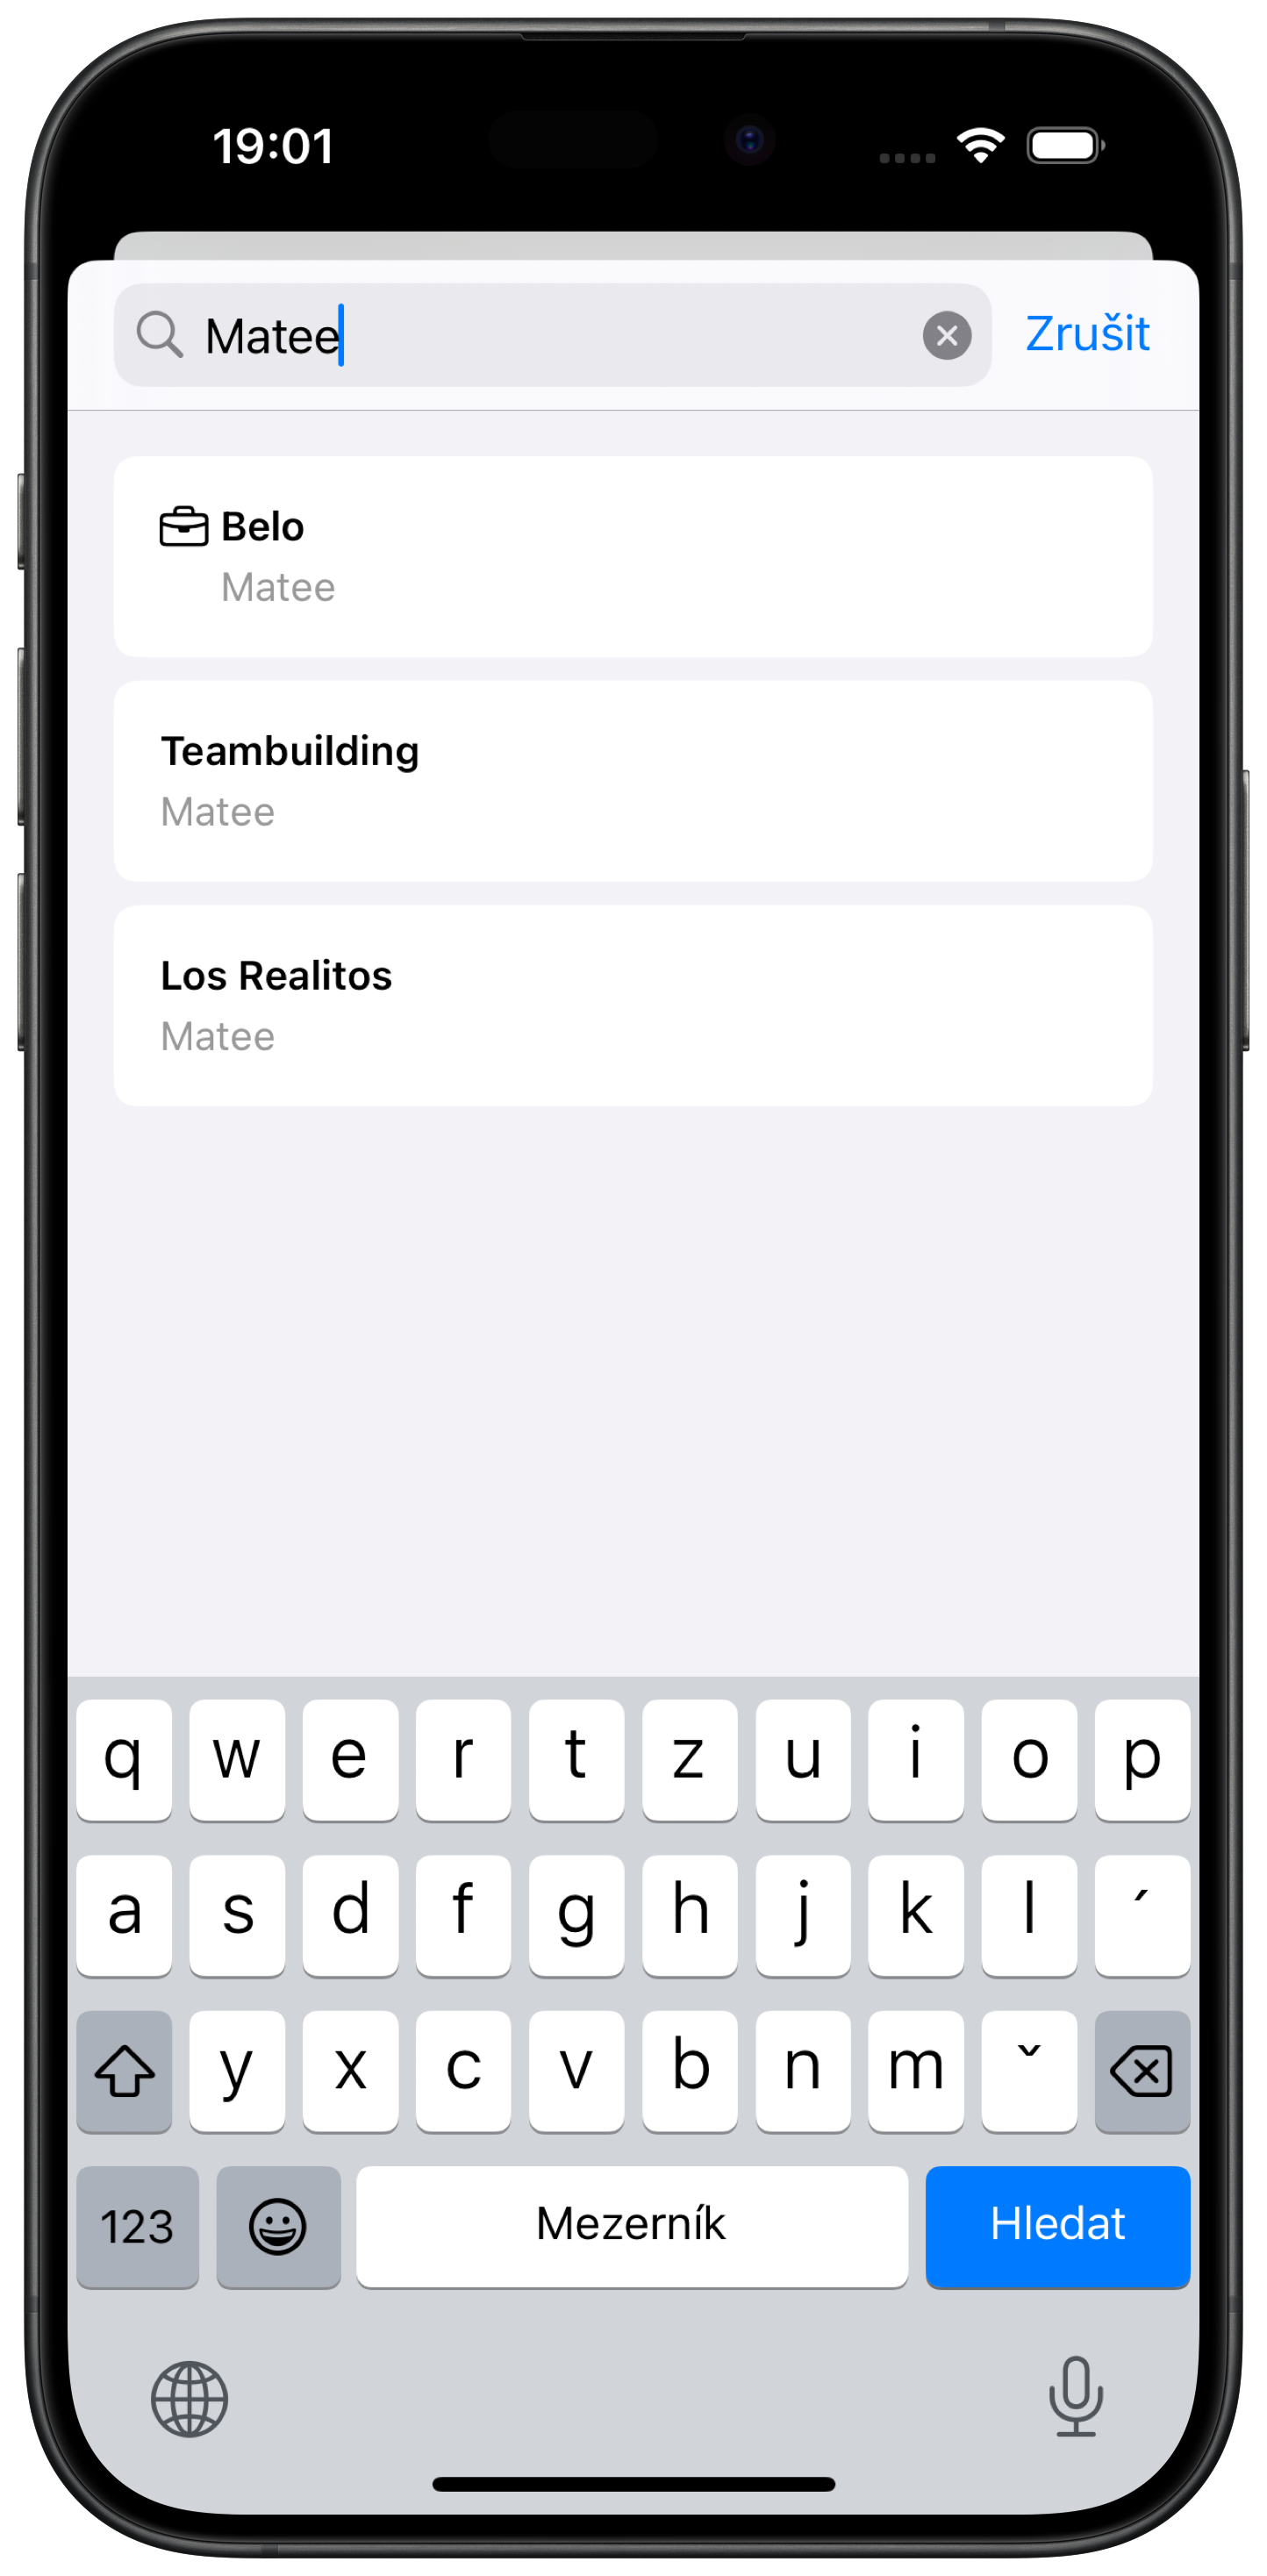
\includegraphics[width=6cm]{project-select-search-impl.png}
		\caption{Vyhledávání}
		\label{fig:project-select-search-impl}
	\end{subfigure}
	\caption{Realizace výběru projektu}
	\label{fig:project-selection-impl}
\end{figure}

Jeden problém, který musí nativní aplikace řešit, je situace, když má zobrazit nově načtenou navazující stránku časových záznamů. Můžou nastat dvě situace – buď nová stránka bude obsahovat data skupiny, která má prázdný průnik s~poslední skupinou již načtených dat (tedy již načtená data neobsahují data nějakého dne, který by neměl plně načtené všechny záznamy), nebo bude tento průnik neprázdný (tedy nová data obsahují data, která se musí spojit s~daty nějakého dne, který je již z~části načtený). Nově načtenou stránku tedy nelze vždy obyčejně připojit za již načtená data, ale musí probíhat kontrola, zda se nějaká skupina z~již načtených dat nemá spojit s~nějakou skupinou nových dat. Multi-platformní část také musí poskytovat data o~tom, zda je jednotlivá skupina již plně načtená. Jediný případ, kdy o~tomto faktu může výstup multi-platformního \emph{Use Case} lhát, je ten, pokud se jedná o~poslední skupinu v~načtených datech, jejíž konec ale přesně končí v~místě, kde končí i~záznamy dalšího dne, což ale \emph{Use Case} nemá jak zjistit. Tento případ musí ručně detekovat nativní aplikace při načtení nové stránky a~opravit skupinu, u~které to mohlo nastat, tak, že jí označí za plně načtenou. Implementace této logiky lze nahlédnout ve výpisu kódu \ref{code:view-mode-entry-group-overlap}.

\begin{listing}
\caption{Obsluha nově načtené navazující stránky záznamů}\label{code:view-mode-entry-group-overlap}
\begin{minted}{Swift}
// Fetch more groups
let fetchedGroups: [TimerEntryGroup] = try await getTimerEntriesUseCase.execute(
    params: params
)

var newGroups: [TimerEntryGroup] = []

// If there is an overlapping group
if let firstOfCurrent = currentGroups.first,
   let lastOfNew = fetchedGroups.last,
   firstOfCurrent.date == lastOfNew.date {
    // Append already fetched groups without the last one
    newGroups.append(contentsOf: fetchedGroups.dropLast())
    
    // Calculate total interval of the overlapping group
    var interval: KotlinLong? {
        if lastOfNew.interval == nil 
            && firstOfCurrent.interval == nil 
        { return nil }
        
        let lastOfNewInterval = lastOfNew.interval?.int ?? 0
        let firstOfCurrentInterval = firstOfCurrent.interval?.int ?? 0
        
        return KotlinLong(
            value: (lastOfNewInterval + firstOfCurrentInterval).int64
        )
    }
    
    // Append union of the overlapping group
    newGroups.append(TimerEntryGroup(
        date: firstOfCurrent.date,
        interval: interval,
        entries: lastOfNew.entries + firstOfCurrent.entries,
        isFullyLoaded: lastOfNew.isFullyLoaded
    ))
    
    // Append the fetched groups without the first one
    newGroups.append(contentsOf: currentGroups.dropFirst())
} else {
    // No overlapping groups, just append
    newGroups.append(contentsOf: fetchedGroups)
    
    // Fix the `isFullyLoaded` flag if necessary
    if let firstOfCurrent = currentGroups.first, !firstOfCurrent.isFullyLoaded {
        firstOfCurrent.isFullyLoaded = true
    }
    newGroups.append(contentsOf: currentGroups)
}

// Display the updated data
state.listData = .data(newGroups)
\end{minted}
\end{listing}

Veškerá ostatní logika spočívá v~přímočarém používání \emph{Use Cases} podle toho, co je úmyslem uživatele. \emph{View Model} této obrazovky si mimo to musí pamatovat ručně zadaný konec záznamu, jelikož ten není součástí aktuálního nastavení časovače, nebo také musí každou sekundu aktualizovat čas, který se ukazuje na běžících stopkách, ale také tento čas přičítat k~souhrnům aktuálního dne a~týdne.

%---------------------------------------------------------------
\subsection{Profil uživatele}
%---------------------------------------------------------------

Tato funkcionalita pokrývá operace, které může uživatel dělat se svým profilem, se svými klienty a~se svými projekty. 

%---------------------------------------------------------------
\subsubsection{Backend}
%---------------------------------------------------------------

Obsluhu požadavků týkajících se projektů bude řešit modul pro projekty, požadavky týkající se klientů bude řešit modul pro klienty a~požadavky týkající se profilu bude řešit modul pro uživatele.

Co se týče funkcí, co může uživatel dělat se svým profilem, tak se na obrazovce profilu může buď odhlásit, nebo si svůj účet smazat.

Odhlášení je čistě autentizační záležitost, probíhá tedy pouze na straně klienta, kde je součástí modulu \texttt{auth}, jak bylo popsáno v~sekci \ref{onboarding-impl}.

Smazání účtu už je ale z~hlediska dat zajímavější záležitost. Během mazání účtu bude potřeba smazat všechna data, která jsou s~uživatelem propojená, tedy všechny jeho záznamy a~integrace. V~první řadě bude tedy potřeba smazat každý dokument v~kolekci \texttt{/entries/\{uid\}/entries}, protože pro smazání kolekce je potřeba smazat každý dokument, nelze smazat celou kolekci najednou. Poté se bude moct smazat dokument \texttt{/entries/\{uid\}}. Poté se budou muset smazat všechny integrace, tedy všechny dokumenty v~kolekci \texttt{/users/\{uid\}/integrations}, poté všechny informace o~tom, jaké klienty a~projekty má uživatel přiřazené, tedy dokumenty v~kolekci \texttt{/users/\{uid\}/clients} a~ve finále se může smazat dokument uživatele, tedy \texttt{/users/\{uid\}}. Tím budou smazána všechna data související s~uživatelem ve \emph{Firestore} databázi. Poté je ještě potřeba smazat uživatele z~\emph{Firebase} autentizace, aby se na něj už nešlo přihlásit. Celou tuto logiku implementuje funkce \texttt{deleteUser(uid: String)} v~\texttt{UserSourceImpl}.

Další, co bude backend muset implementovat, jsou všechny CRUD (Create, Read, Update, Delete) operace pro klienty a~projekty. Za to mají odpovědnost příslušné \texttt{ProjectRepository}, \texttt{ClientRepository} a~jejich \emph{Sources}. Specifikem projektů je, že pro jejich jednoznačnou identifikaci nestačí pouze identifikátor projektu, ale je potřeba i~identifikátor klienta, ke kterému patří. Také je potřeba implementovat funkce pro přečtení všech klientů pro konkrétního uživatele a~přečtení všech projektů daného uživatele. Poté je také potřeba poskytnout API pro přiřazení klienta nebo projektu k~uživateli, samotné vytvoření je totiž pouze zařadí do kolekcí, ale nepřiřadí je k~žádnému uživateli. Implementace \emph{Route}, která obsluhuje přiřazení projektu k~uživateli, lze nahlédnout ve výpisu kódu \ref{code:be-route-assign-project}. Toto přiřazení řeší speciální \emph{PUT endpoint}, který nepřijímá žádné tělo požadavku.

\begin{listing}
\caption{\emph{Route} pro přiřazení klienta k~uživateli}\label{code:be-route-assign-project}
\begin{minted}{Kotlin}
fun Routing.userRoute() {

    // ...
    
    authenticate {
    
        // ...
        
        route("/user") {
        
            // ...
            
            route("/projects") {
            
                // ...
                
                put("/add") {
                    val user = call.requireUserPrincipal().user
                    val clientId: String by call.request.queryParameters
                    val projectId: String by call.request.queryParameters

                    userRepository.assignProjectToUser(user.uid, clientId, projectId)

                    call.respond(HttpStatusCode.OK)
                }
            }
            
            // ...
            
        }
    }
}
\end{minted}
\end{listing}

Úprava a~mazání projektů a~klientů je také poměrně komplexní záležitost, jelikož je spolu s~nimi potřeba upravit nebo smazat řadu dat, které s~nimi souvisí. Například, pokud se u~upravovaného projektu změní klient, ke kterému patří, bude potřeba změnit všechny časové záznamy, které tento projekt obsahují, aby měly identifikátor nového klienta, dále je potřeba u~všech uživatelů, kteří měli tento projekt přiřazený, toto přiřazení přesunout z~dokumentu původního klienta do dokumentu nového klienta, je potřeba samotný projekt přesunout do kolekce nového klienta, a~ověřit aktuální data časovače u~všech uživatelů, protože tam tento projekt se starým klientem může být. Podobně složité může být například mazání klienta. Spolu s~ním je totiž potřeba smazat u~všech uživatelů případná přiřazení tohoto klienta a~jeho projektů, smazat všechny projekty, které ke klientovi patří, smazání všech časových záznamů všech uživatelů, kteří mají tohoto klienta přiřazeného, a~až poté smazat klienta. Všechnu tuto logiku definují implementace jednotlivých \emph{Sources}, tedy \texttt{ProjectSourceImpl} a~\texttt{ClientSourceImpl}.

%---------------------------------------------------------------
\subsubsection{Multi-platformní část}
%---------------------------------------------------------------

Multi-platformní část aplikace poskytuje \emph{Use Cases} pro všechny funkce popsané výše, tedy:
\begin{itemize}
\item\texttt{AddAndAssignClientUseCase} – Přiřadí klienta k~přihlášenému uživateli.
\item\texttt{AddAndAssignProjectUseCase} – Přiřadí projekt k~přihlášenému uživateli.
\item\texttt{DeleteUserUseCase} – Smaže uživatele podle identifikátoru.
\item\texttt{GetClientsUseCase} – Získá všechny klienty přiřazené k~přihlášenému uživateli.
\item\texttt{GetClientUseCase} – Získá klienta podle jeho identifikátoru.
\item\texttt{GetProjectPreviewUseCase} – Získá \emph{preview} objekt pro projekt podle jeho identifikátoru.
\item\texttt{GetUserEmailUseCase} – Získá e-mail přihlášeného uživatele, který se pak zobrazuje v~obrazovce profilu. Tuto informaci nezískává z~backendu, ale pomocí \emph{Firebase} autentizace. E-mail uživatele není ve \emph{Firestore} databázi vůbec uložen, jedná se pouze o~autentizační nástroj.
\item\texttt{RemoveClientUseCase} – Smaže klienta podle identifikátoru.
\item\texttt{RemoveProjectUseCase} – Smaže projekt podle identifikátoru.
\item\texttt{UpdateClientUseCase} – Aktualizuje klienta.
\item\texttt{UpdateProjectUseCase} – Aktualizuje projekt.
\end{itemize}

%---------------------------------------------------------------
\subsubsection{Nativní aplikace}
%---------------------------------------------------------------

Realizace profilu v~iOS aplikaci dodržuje návrh ze sekce \ref{feature-profile}. Na obrázku \ref{fig:profile-impl} lze nahlédnout přehled profilu a~dialog, který se zobrazí při pokusu o~smazání účtu. Na obrázku \ref{fig:clients-impl} lze poté vidět seznam klientů, které má uživatel přiřazené, a~možnost v~nich vyhledávat. Dále lze na obrázku \ref{fig:client-projet-detail-impl} vidět detaily klienta a~projektu, obrázek \ref{fig:project-detail-impl} navíc ukazuje stav detailu během ukládání změn, během kterého s~prvky nelze interagovat. Poslední obrázek \ref{fig:project-list-client-selection-impl} poté znázorňuje seznam projektů a~výběr klienta k~projektu.

\begin{figure}[p]
    \centering
    \begin{subfigure}[b]{0.4\textwidth}
		\centering
		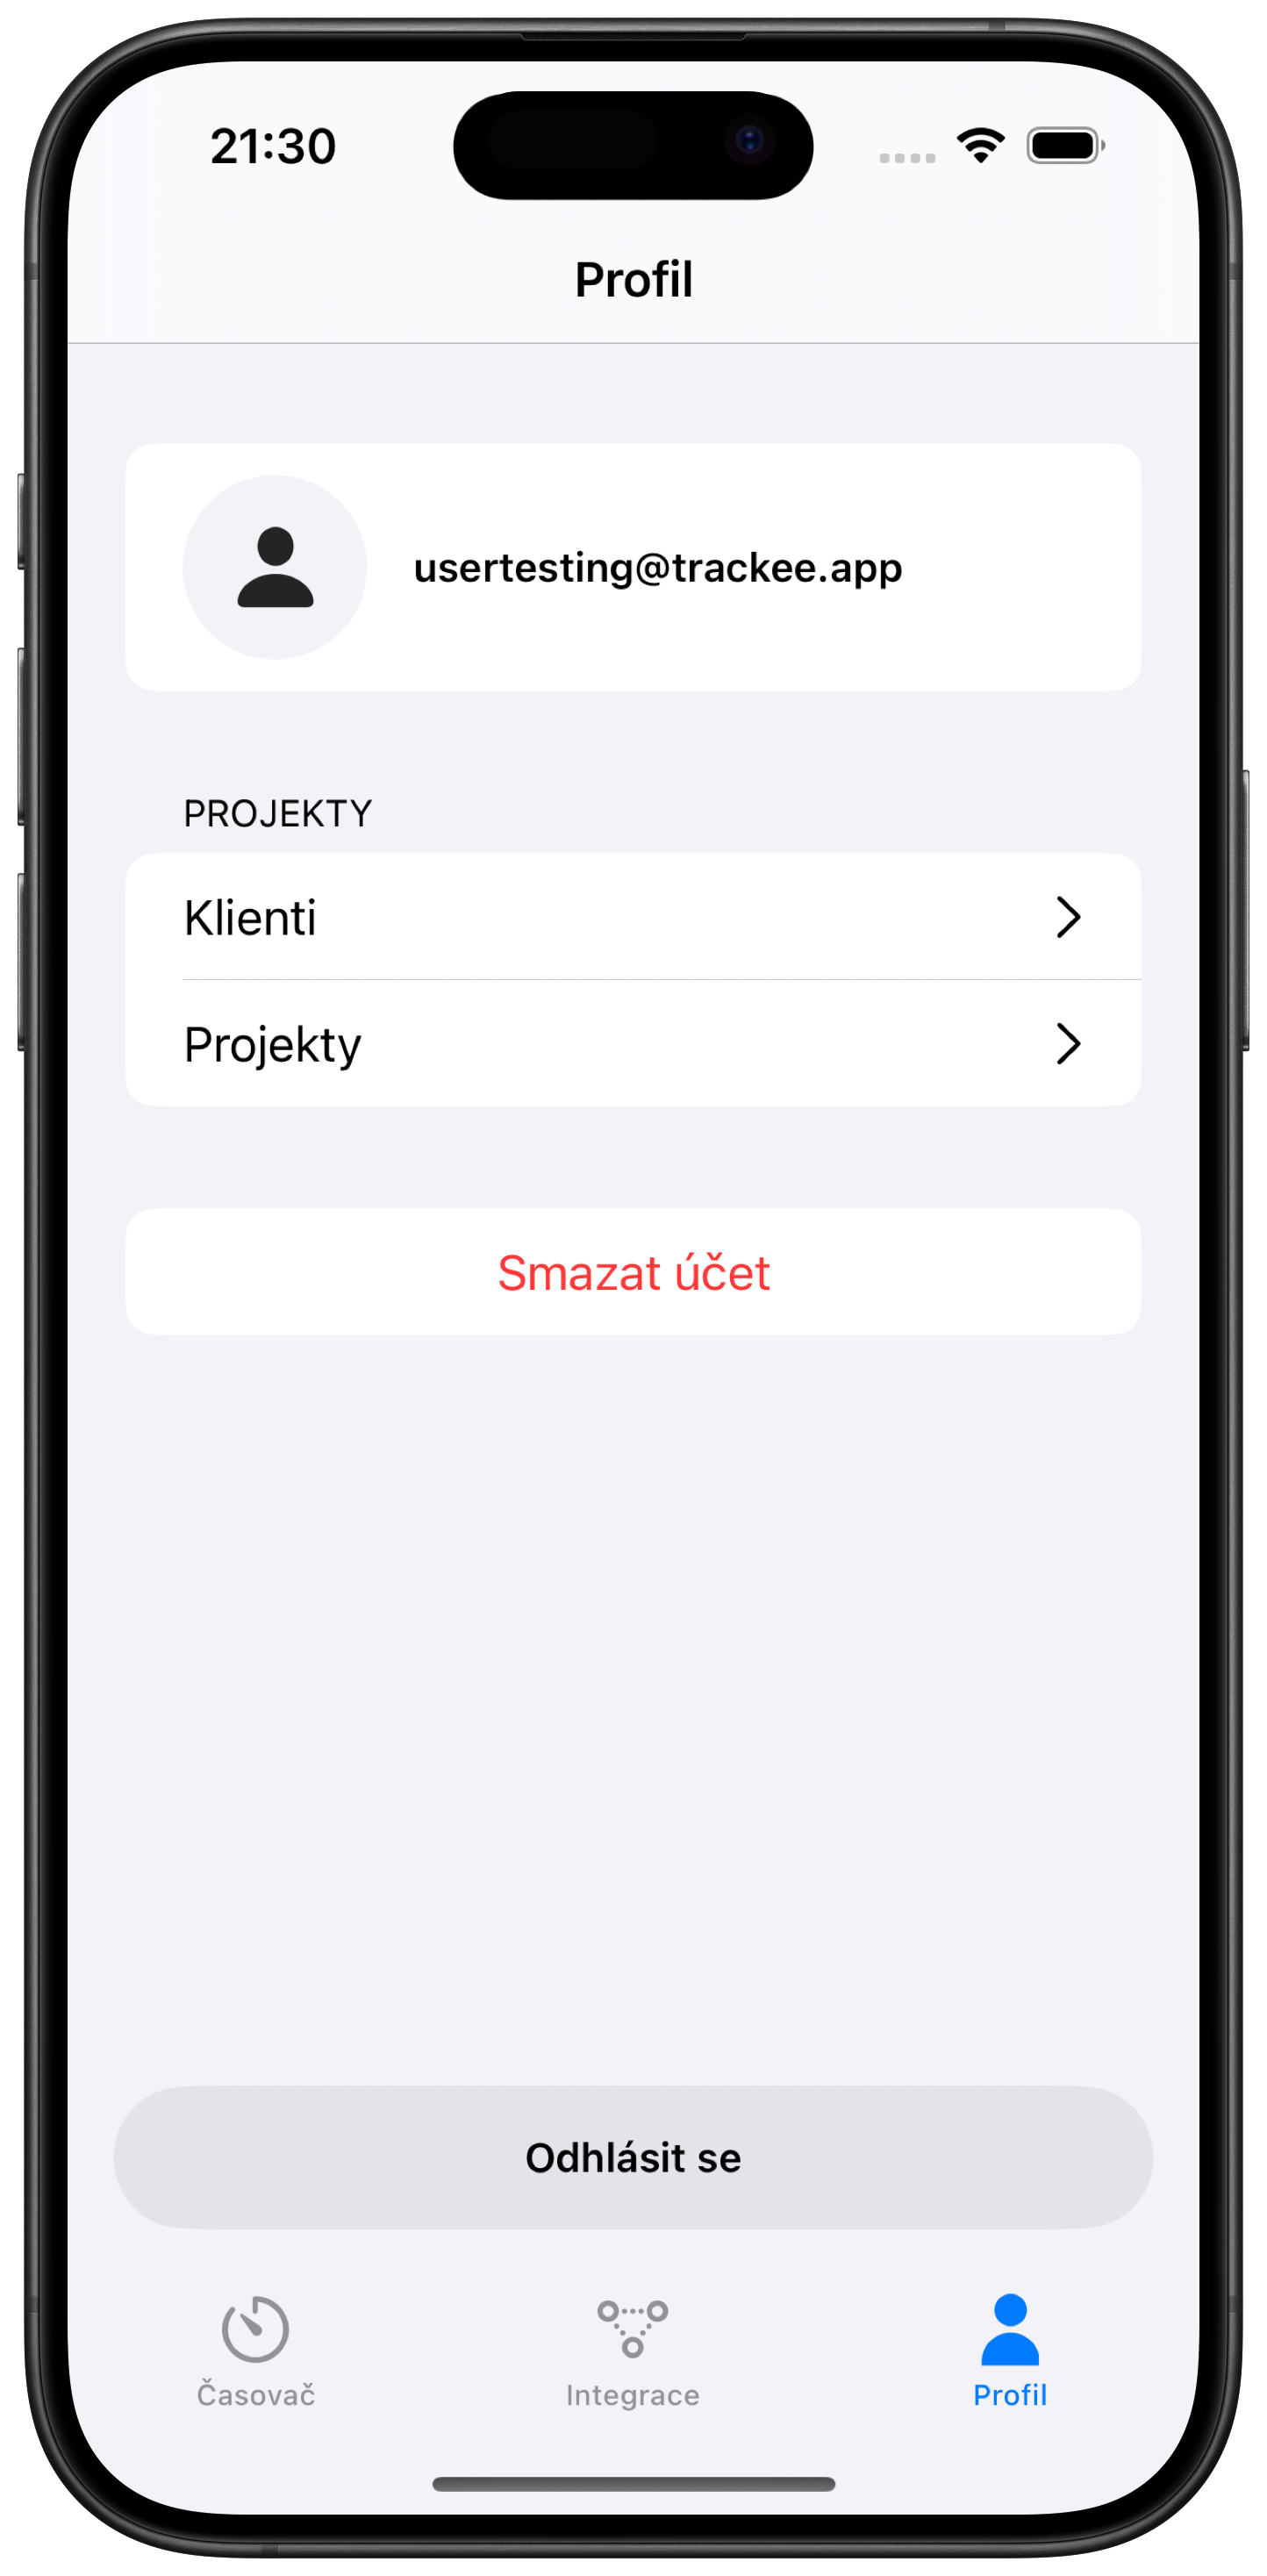
\includegraphics[width=6cm]{profile-impl.png}
		\caption{Přehled}
		\label{fig:profile-overview-impl}
	\end{subfigure}
	\hspace{2cm}
	\begin{subfigure}[b]{0.4\textwidth}
		\centering
		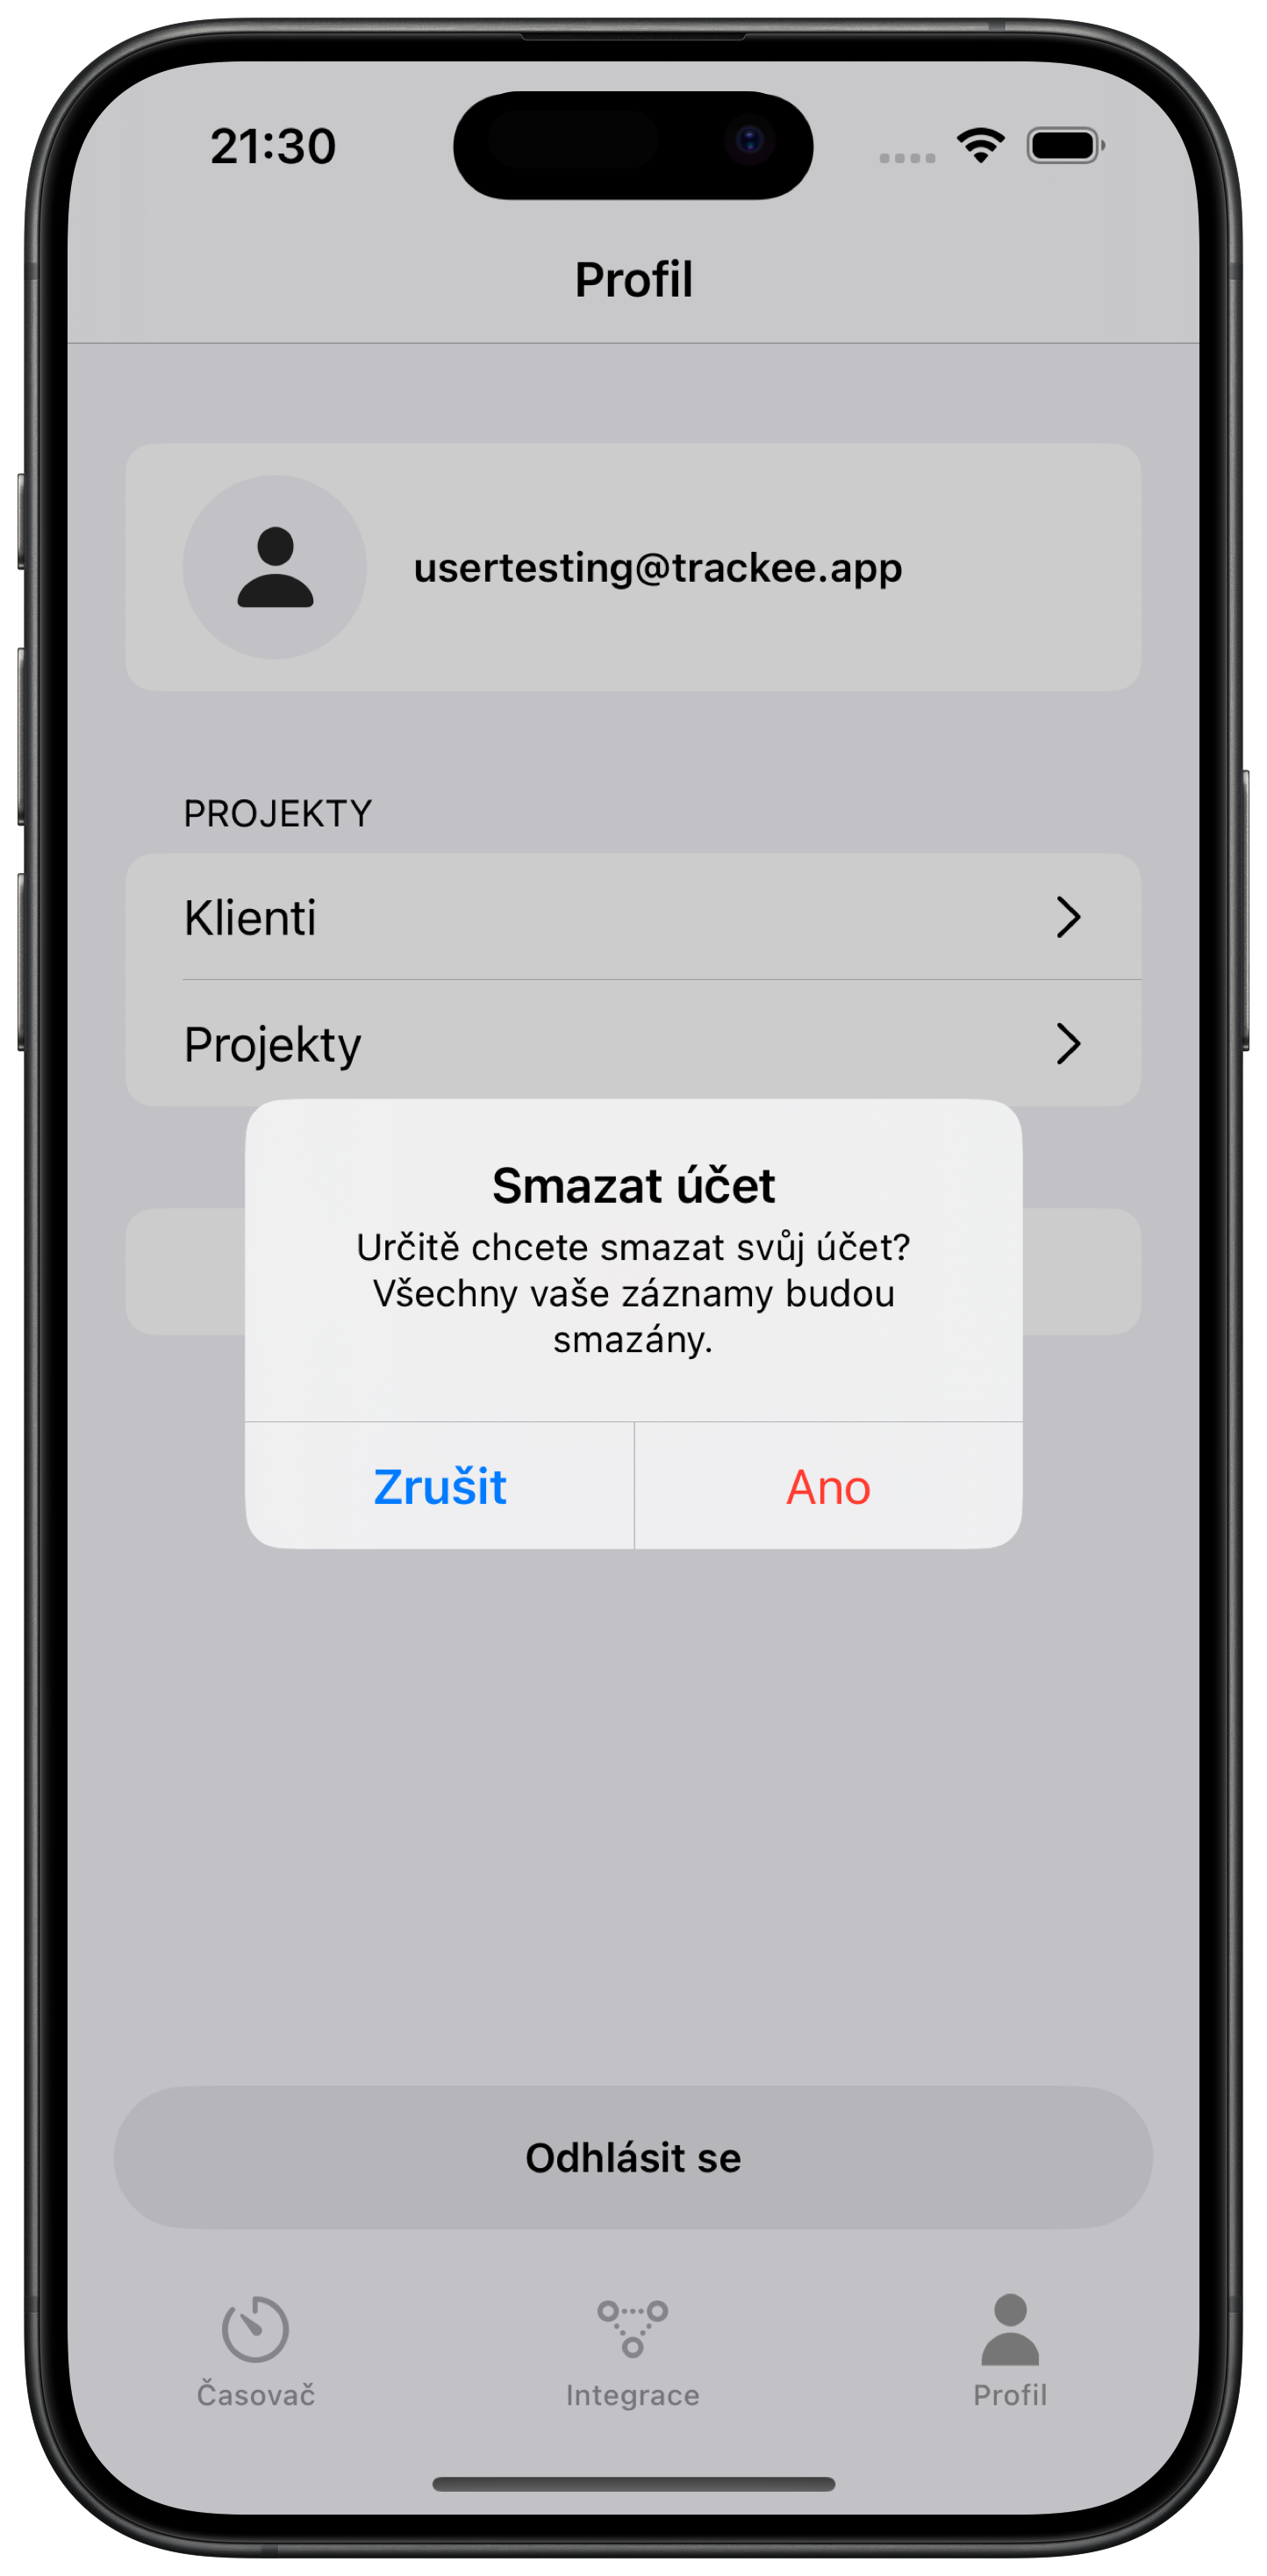
\includegraphics[width=6cm]{profile-delete-impl.png}
		\caption{Dialog pro smazání účtu}
		\label{fig:profile-delete-impl}
	\end{subfigure}
	\caption{Realizace profilu}
	\label{fig:profile-impl}
\end{figure}

\begin{figure}[p]
    \centering
    \begin{subfigure}[b]{0.4\textwidth}
		\centering
		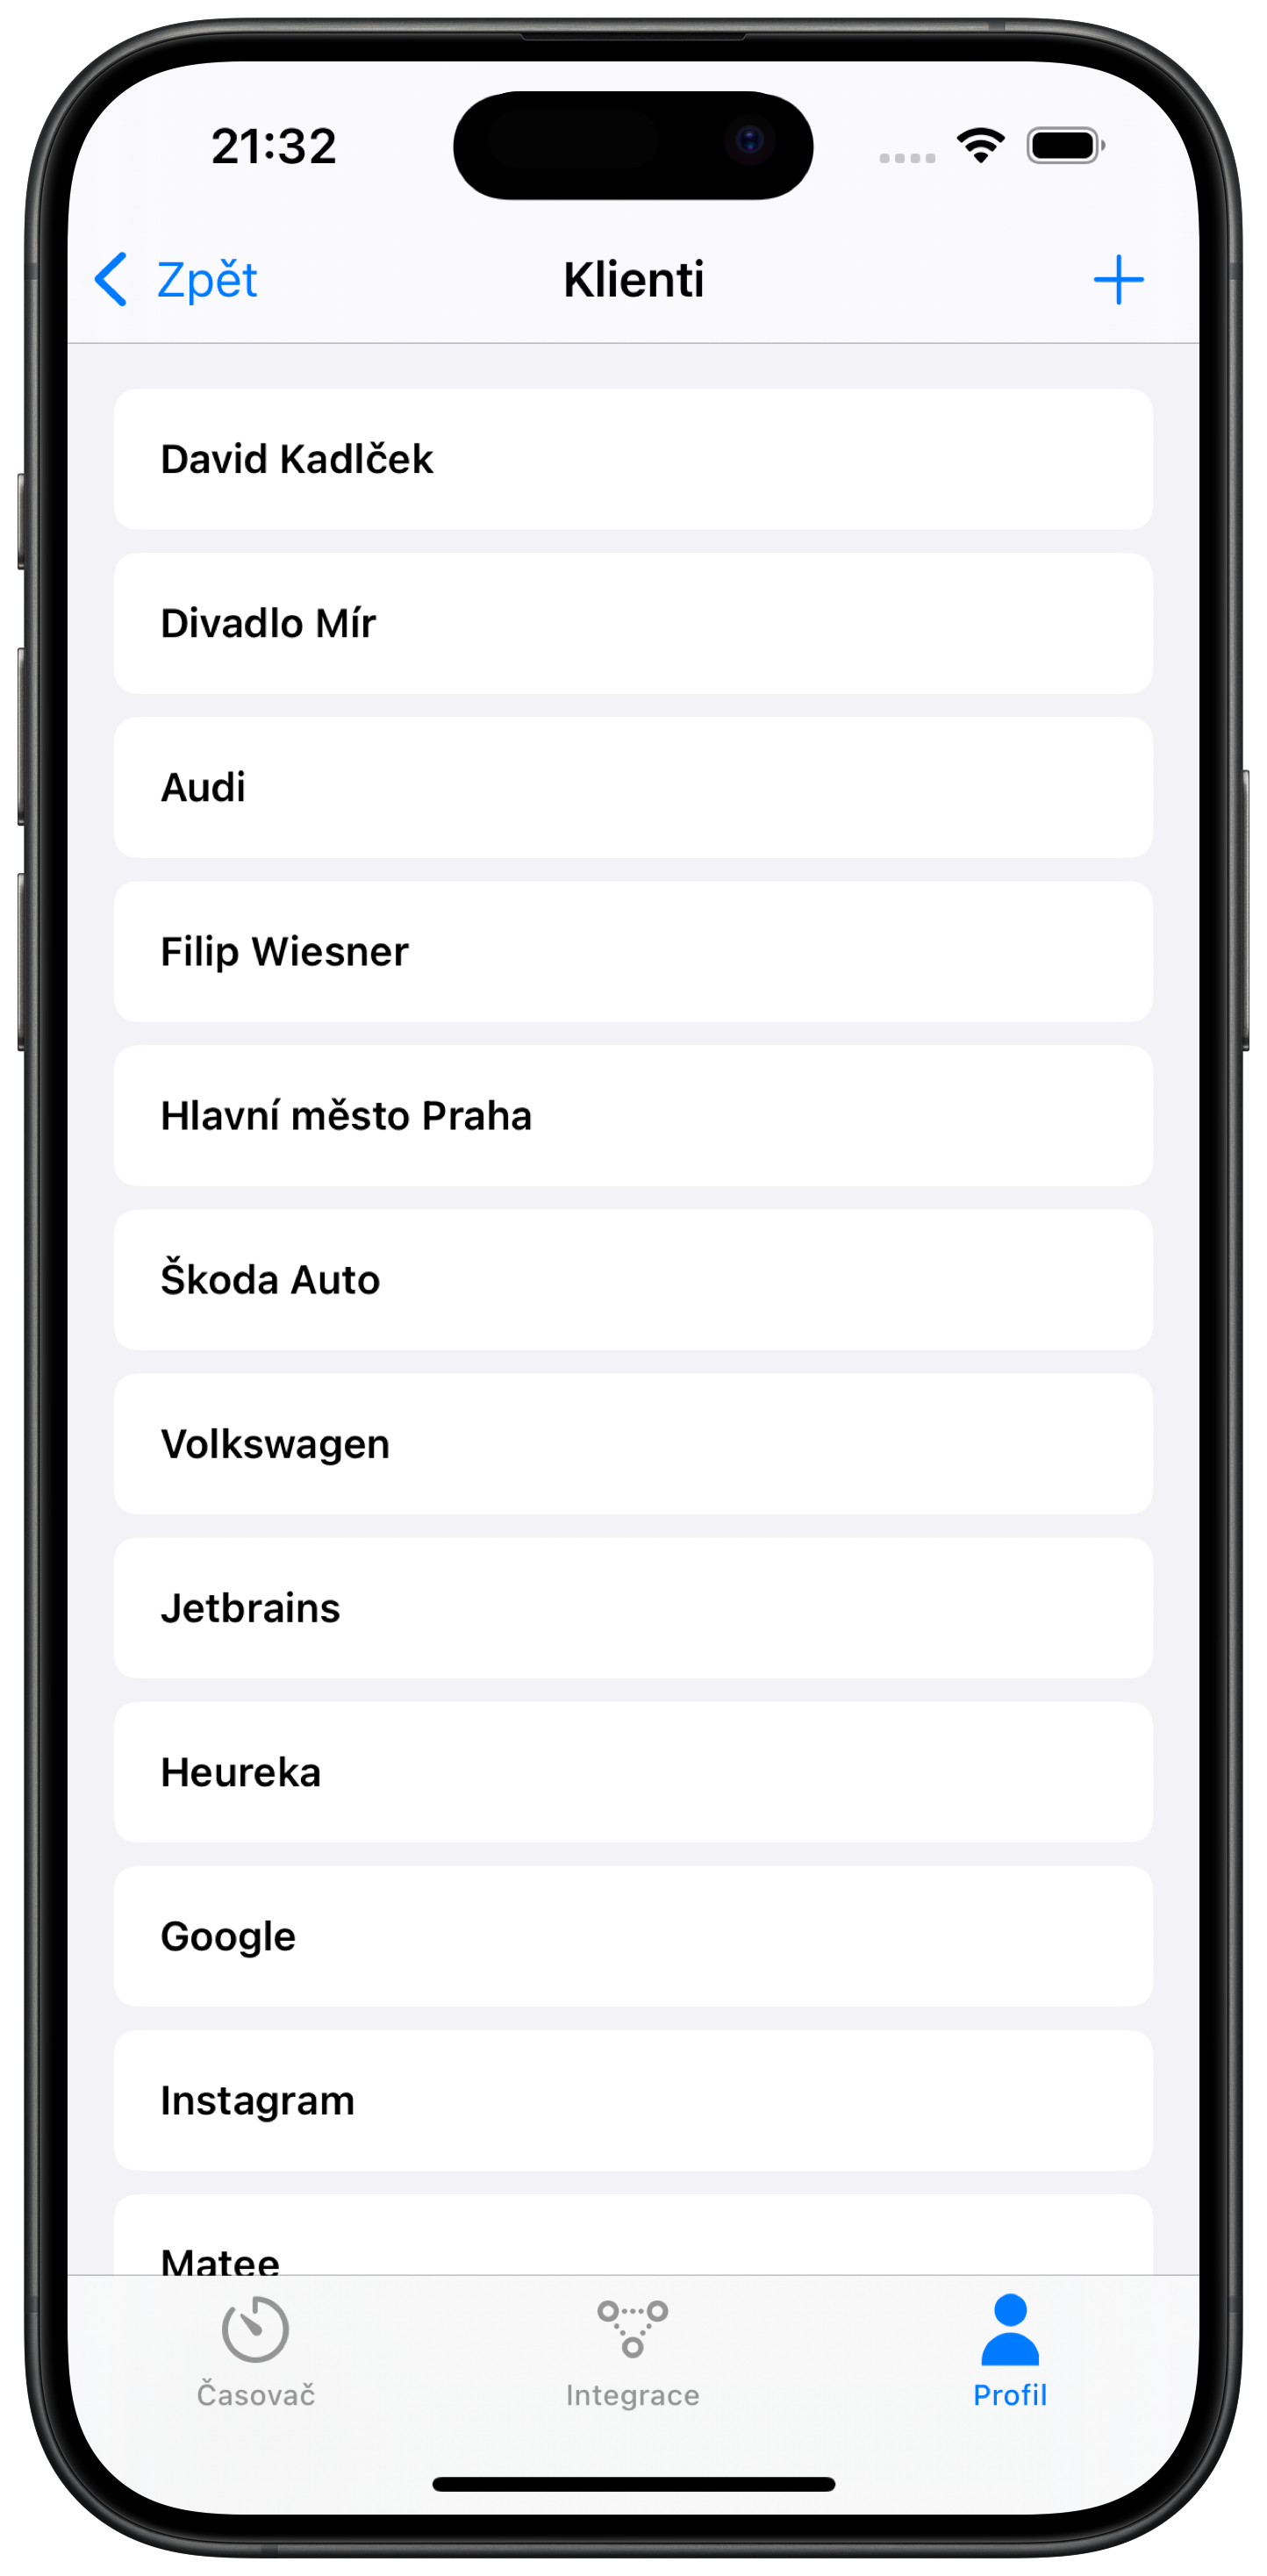
\includegraphics[width=6cm]{client-list-impl.png}
		\caption{Seznam}
		\label{fig:client-list-impl}
	\end{subfigure}
	\hspace{2cm}
	\begin{subfigure}[b]{0.4\textwidth}
		\centering
		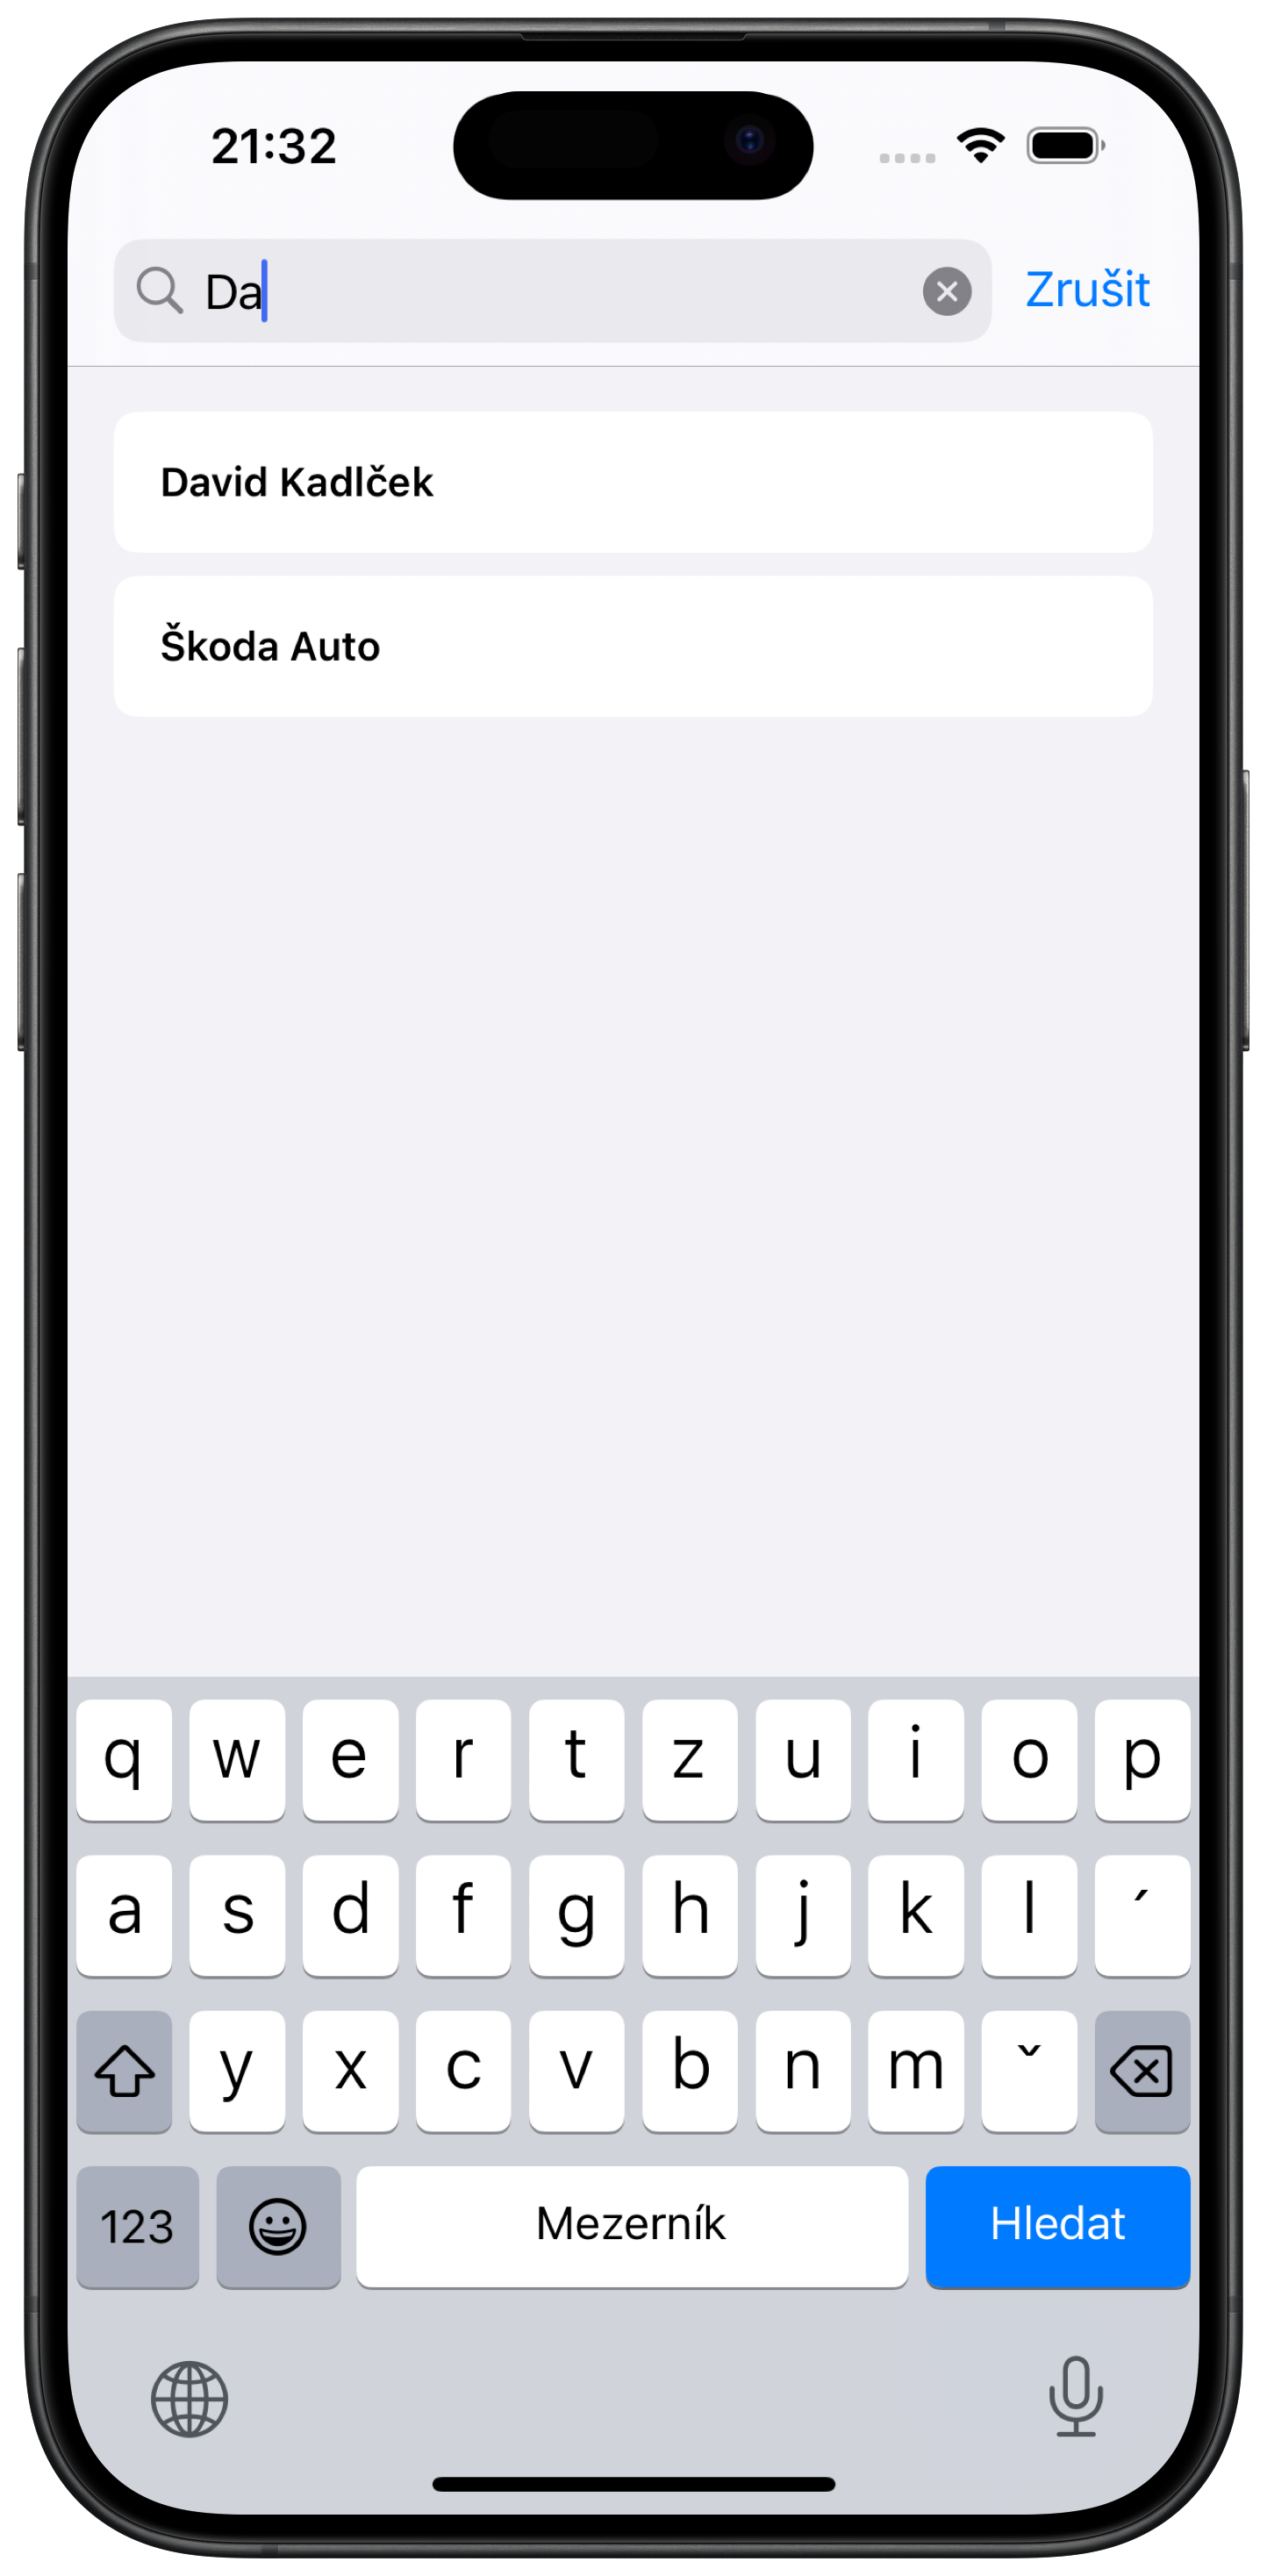
\includegraphics[width=6cm]{client-search-impl.png}
		\caption{Vyhledávání}
		\label{fig:client-search-impl}
	\end{subfigure}
	\caption{Realizace klientů}
	\label{fig:clients-impl}
\end{figure}

\begin{figure}[p]
    \centering
    \begin{subfigure}[b]{0.4\textwidth}
		\centering
		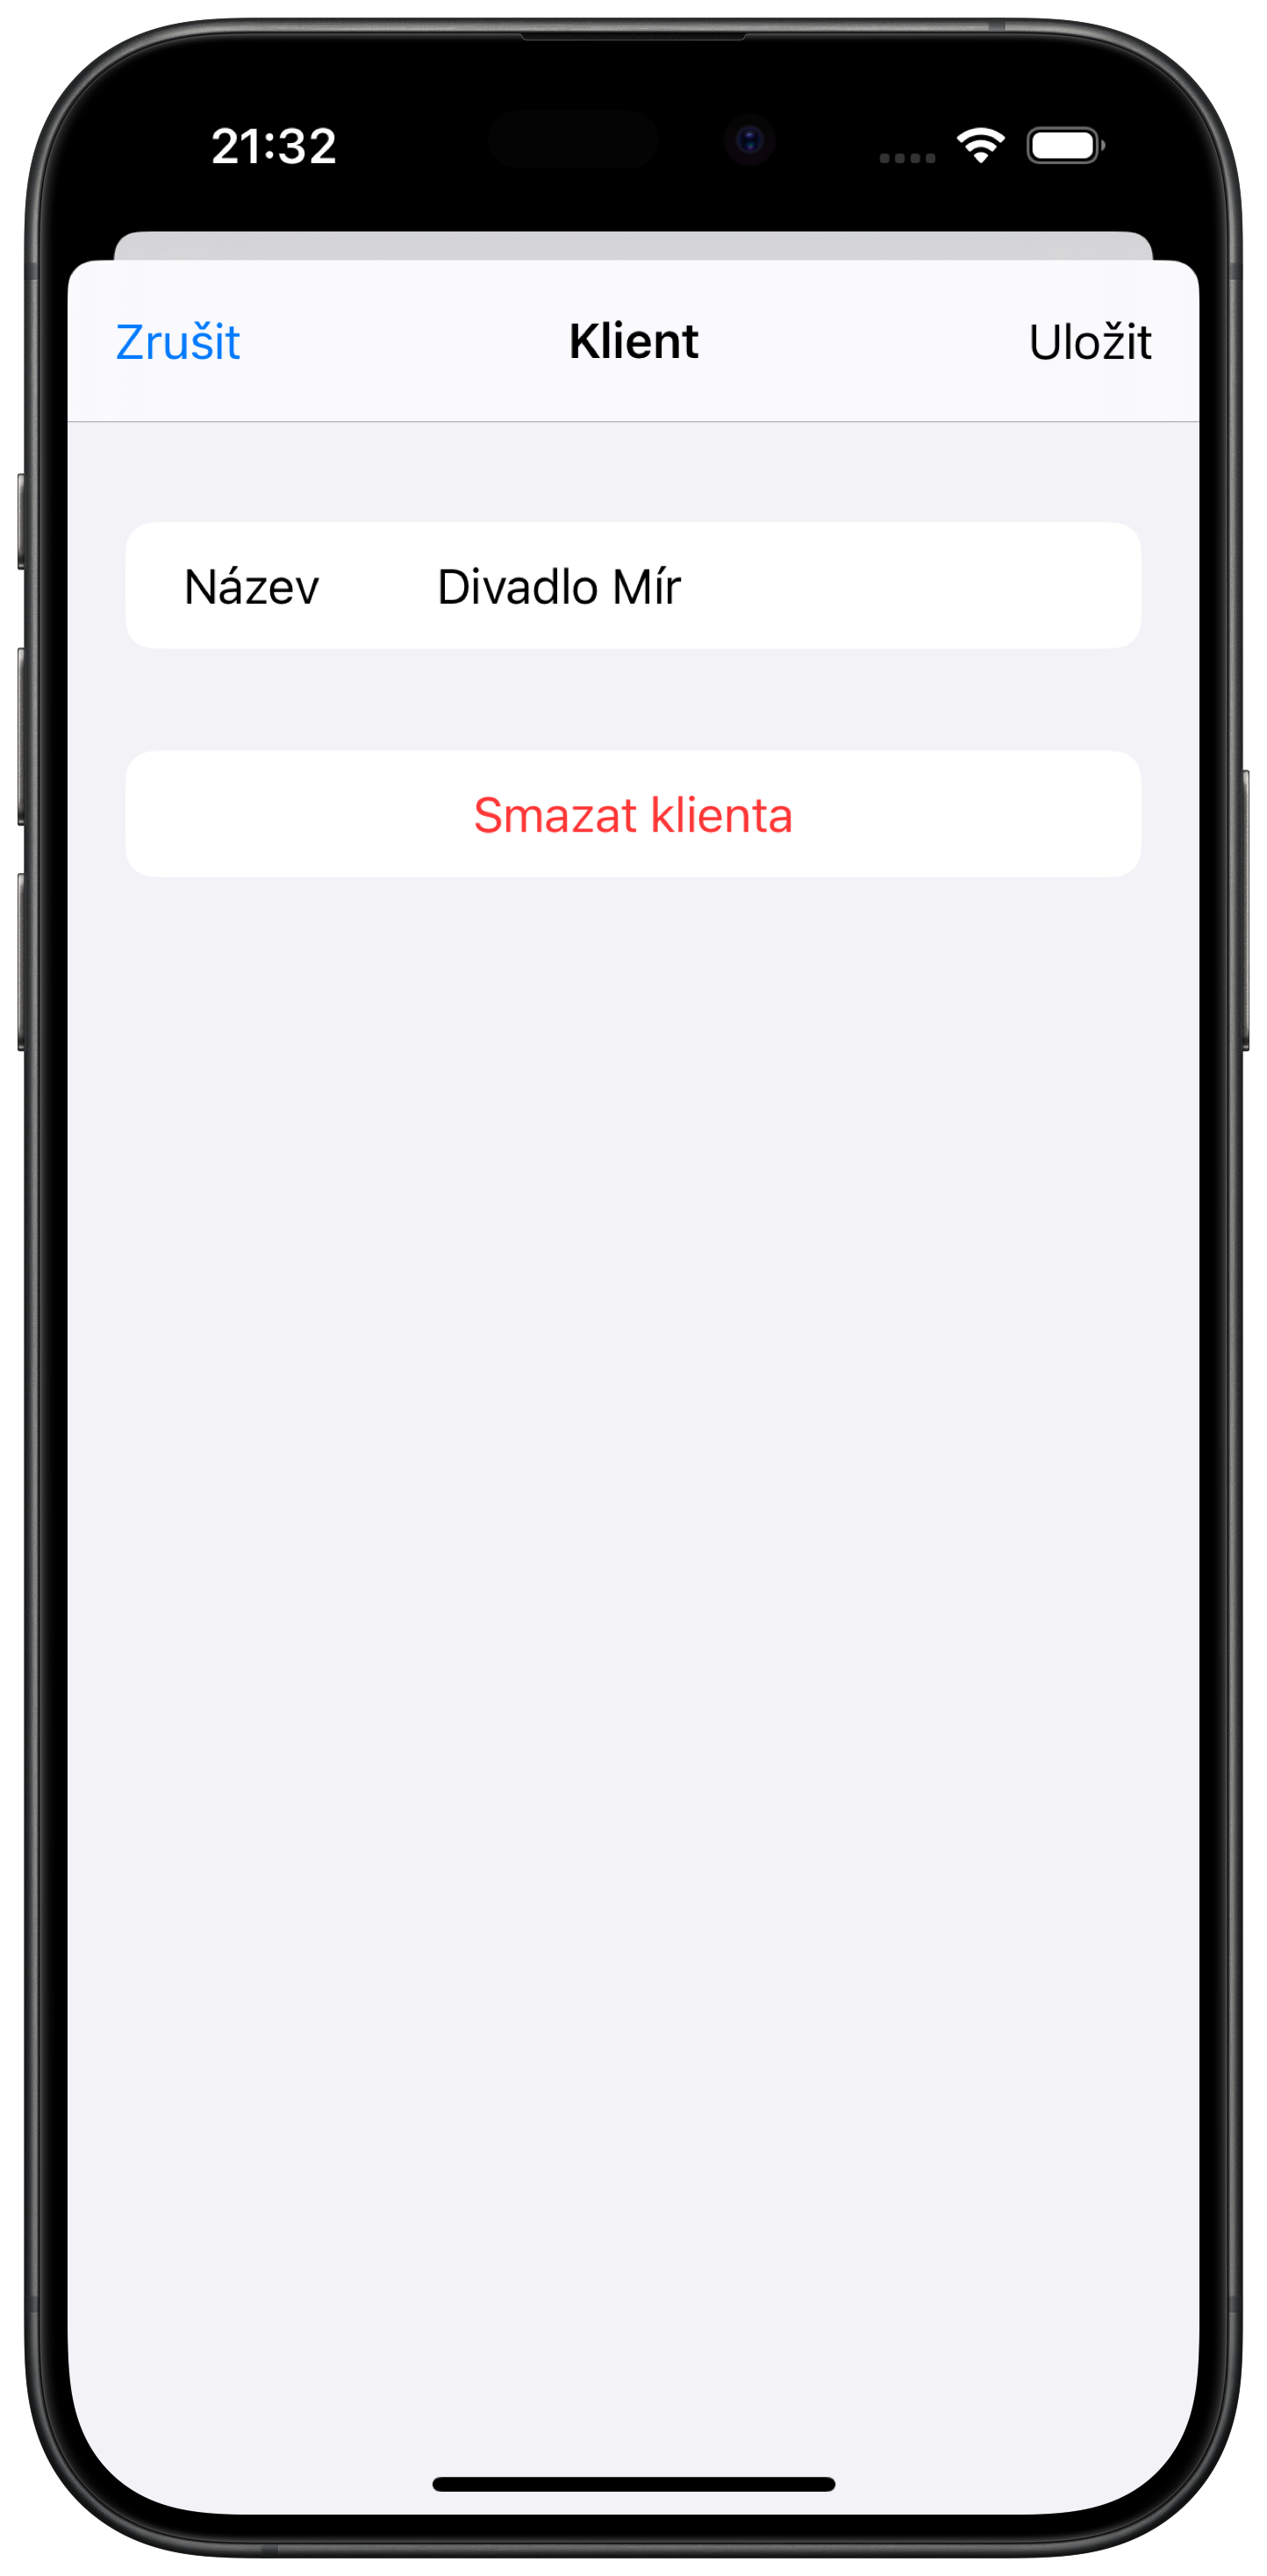
\includegraphics[width=6cm]{client-detail-impl.png}
		\caption{Detail klienta}
		\label{fig:client-detail-impl}
	\end{subfigure}
	\hspace{2cm}
	\begin{subfigure}[b]{0.4\textwidth}
		\centering
		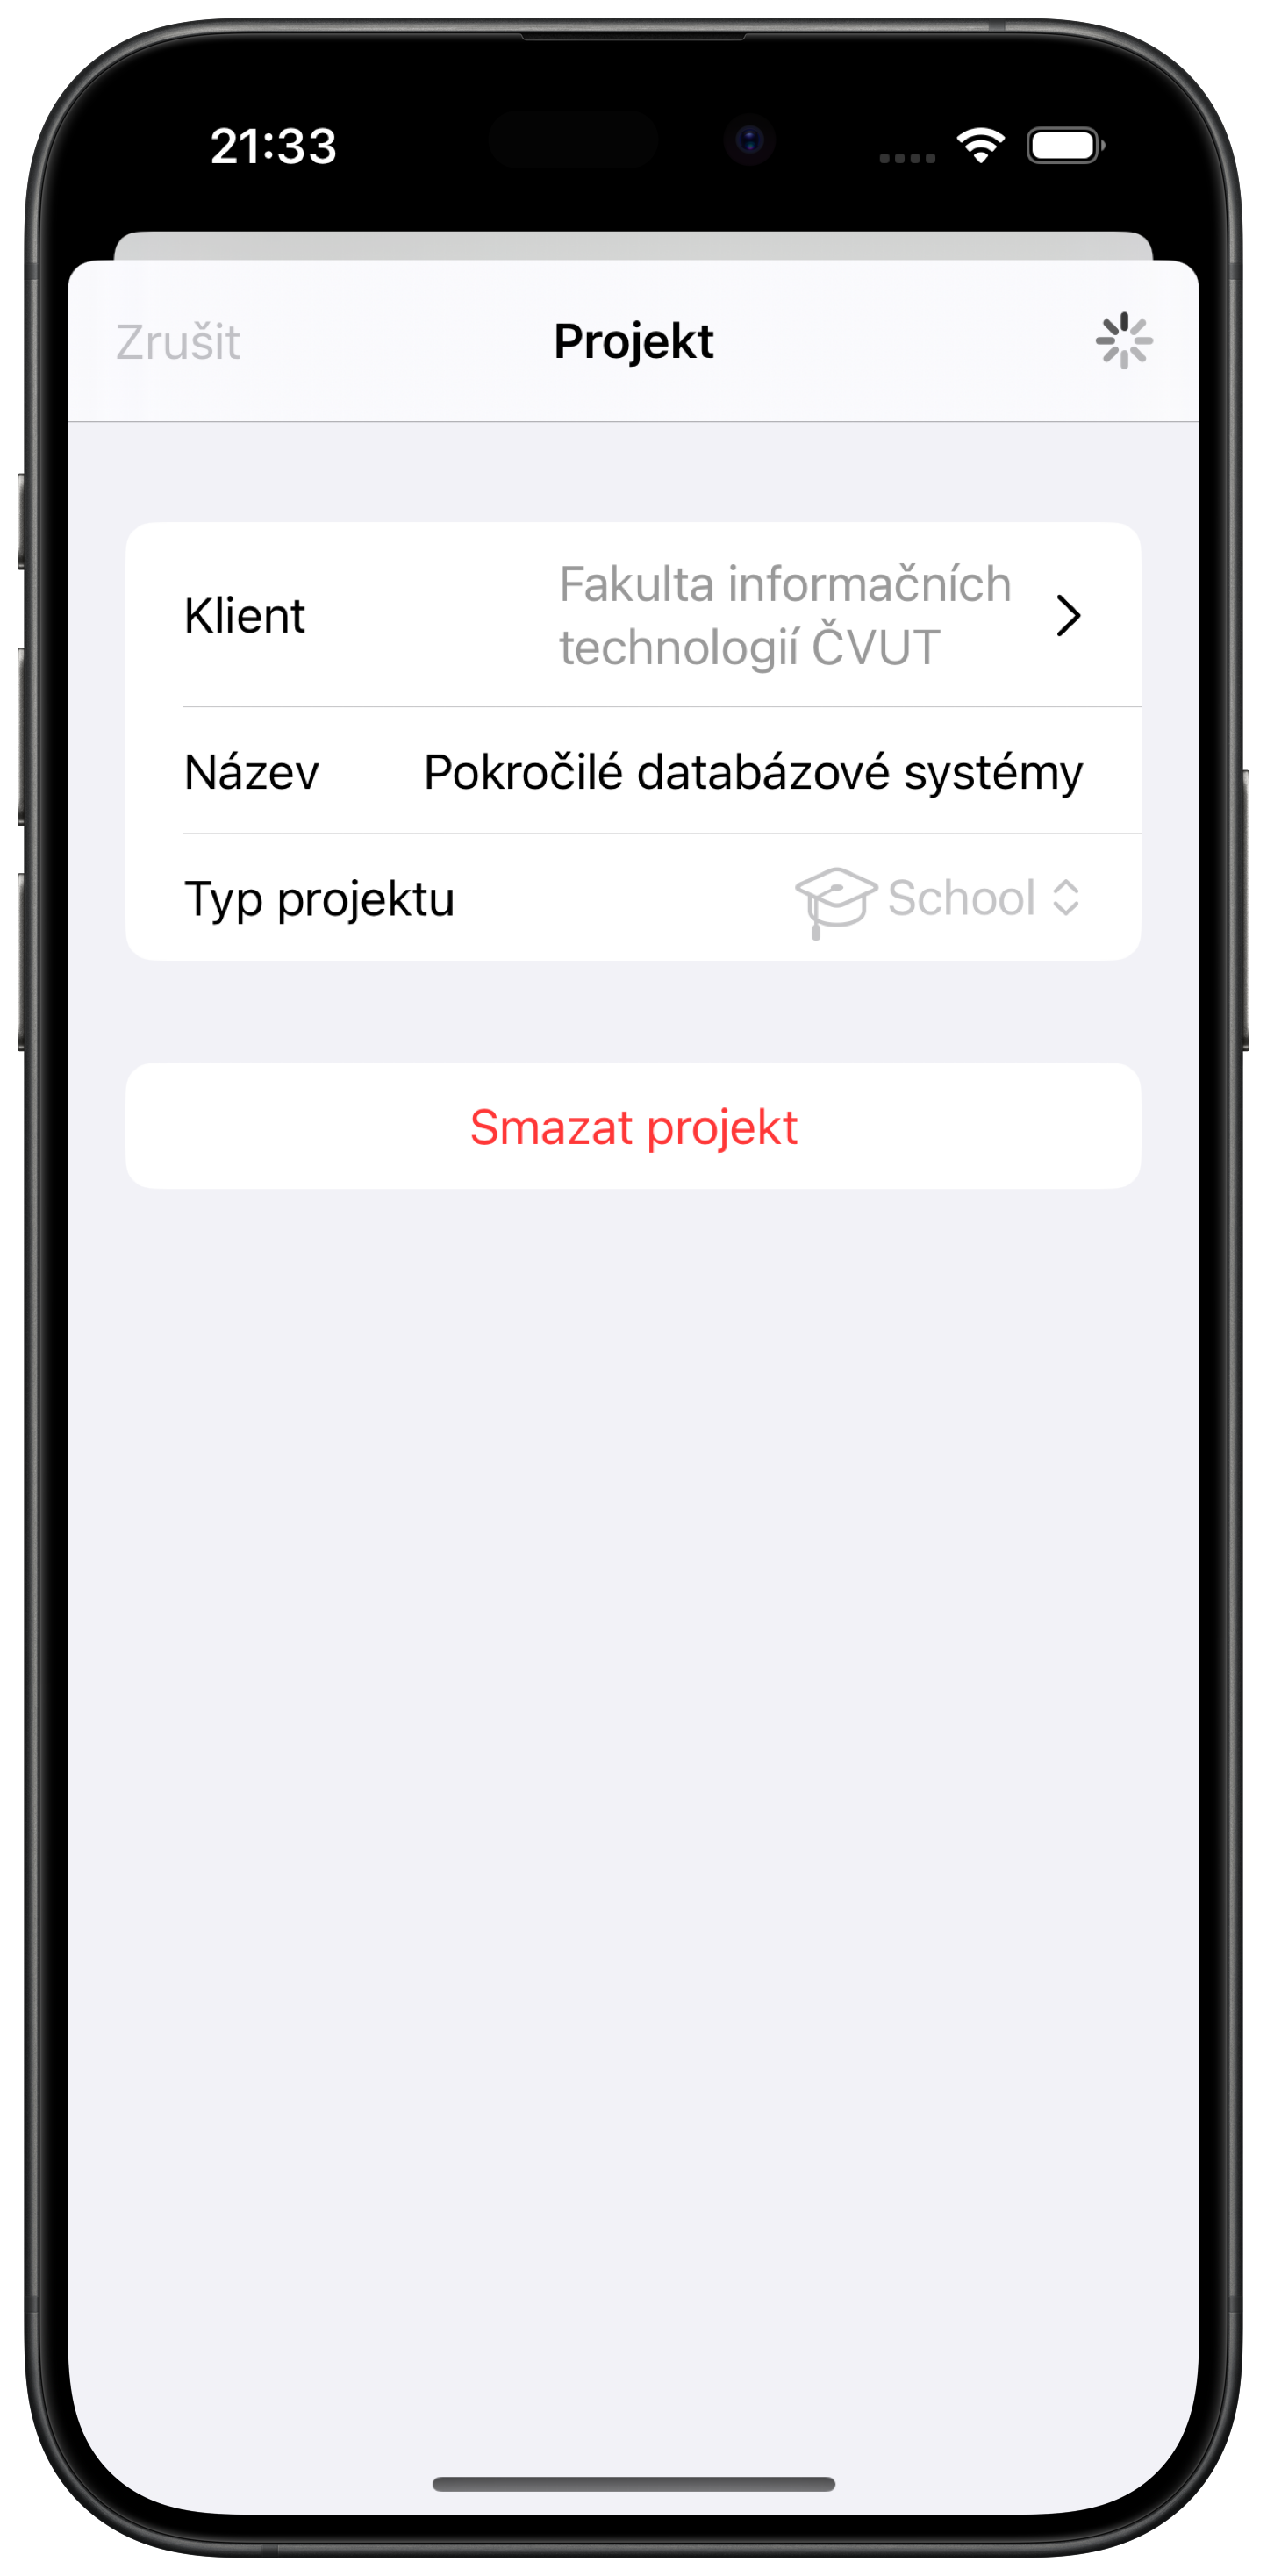
\includegraphics[width=6cm]{project-detail-impl.png}
		\caption{Detail projektu během ukládání}
		\label{fig:project-detail-impl}
	\end{subfigure}
	\caption{Detail klienta a~projektu}
	\label{fig:client-projet-detail-impl}
\end{figure}

\begin{figure}[p]
    \centering
    \begin{subfigure}[b]{0.4\textwidth}
		\centering
		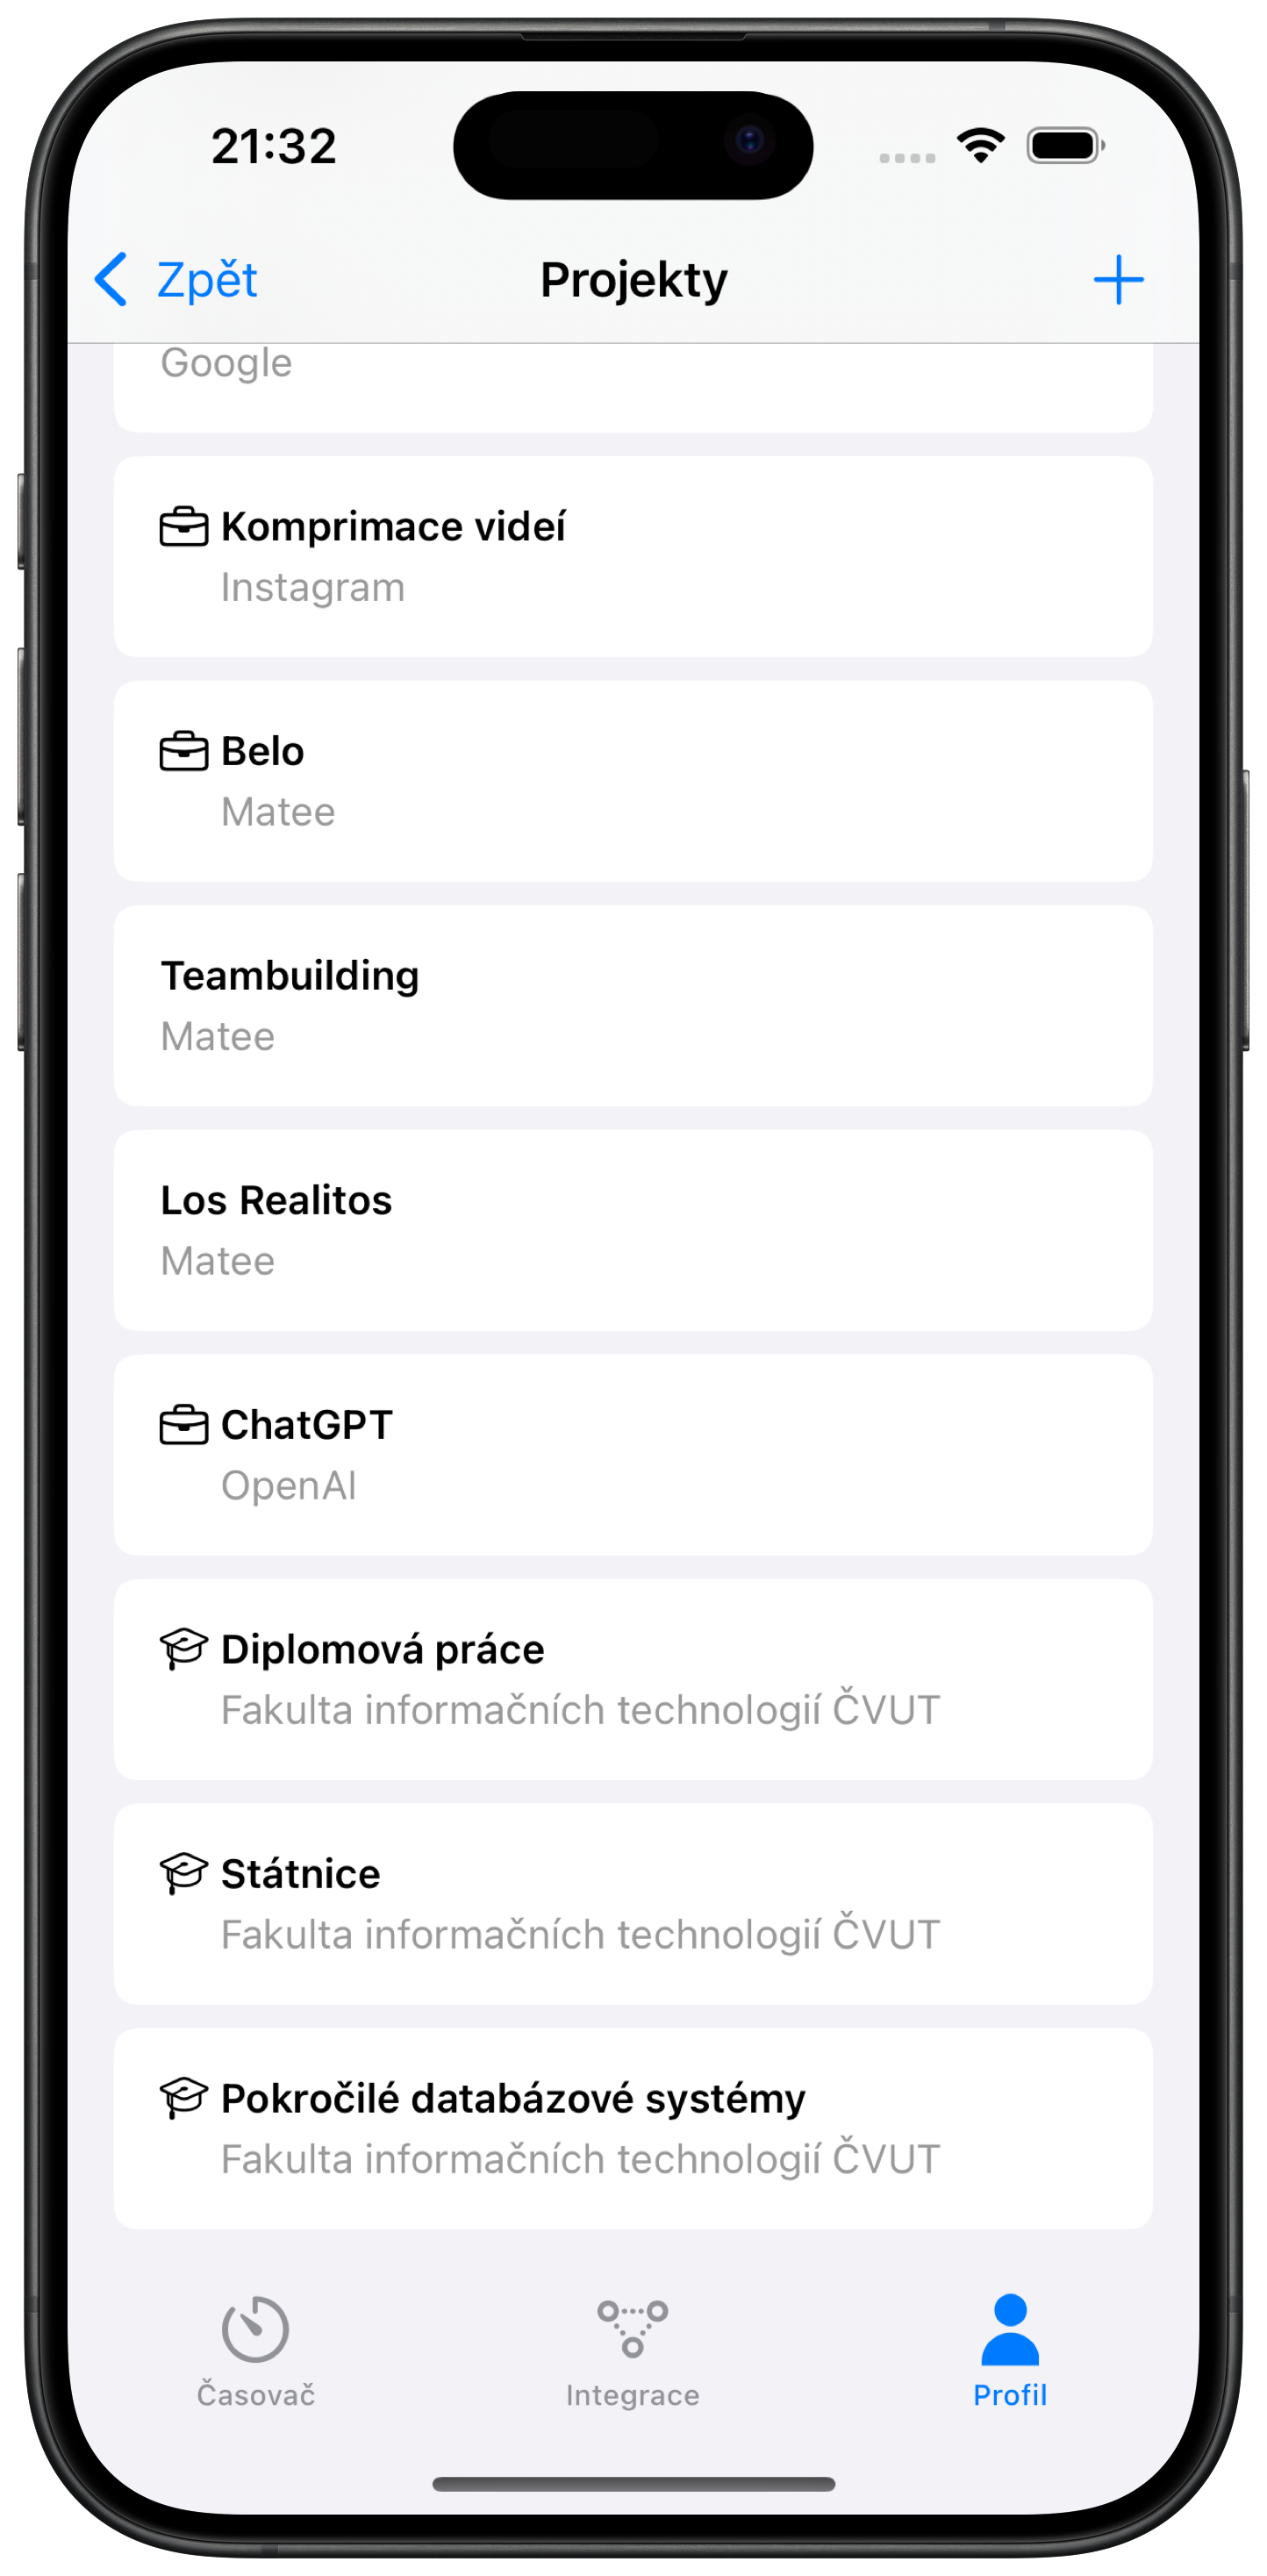
\includegraphics[width=6cm]{project-list-impl.png}
		\caption{Seznam projektů}
		\label{fig:project-list-impl}
	\end{subfigure}
	\hspace{2cm}
	\begin{subfigure}[b]{0.4\textwidth}
		\centering
		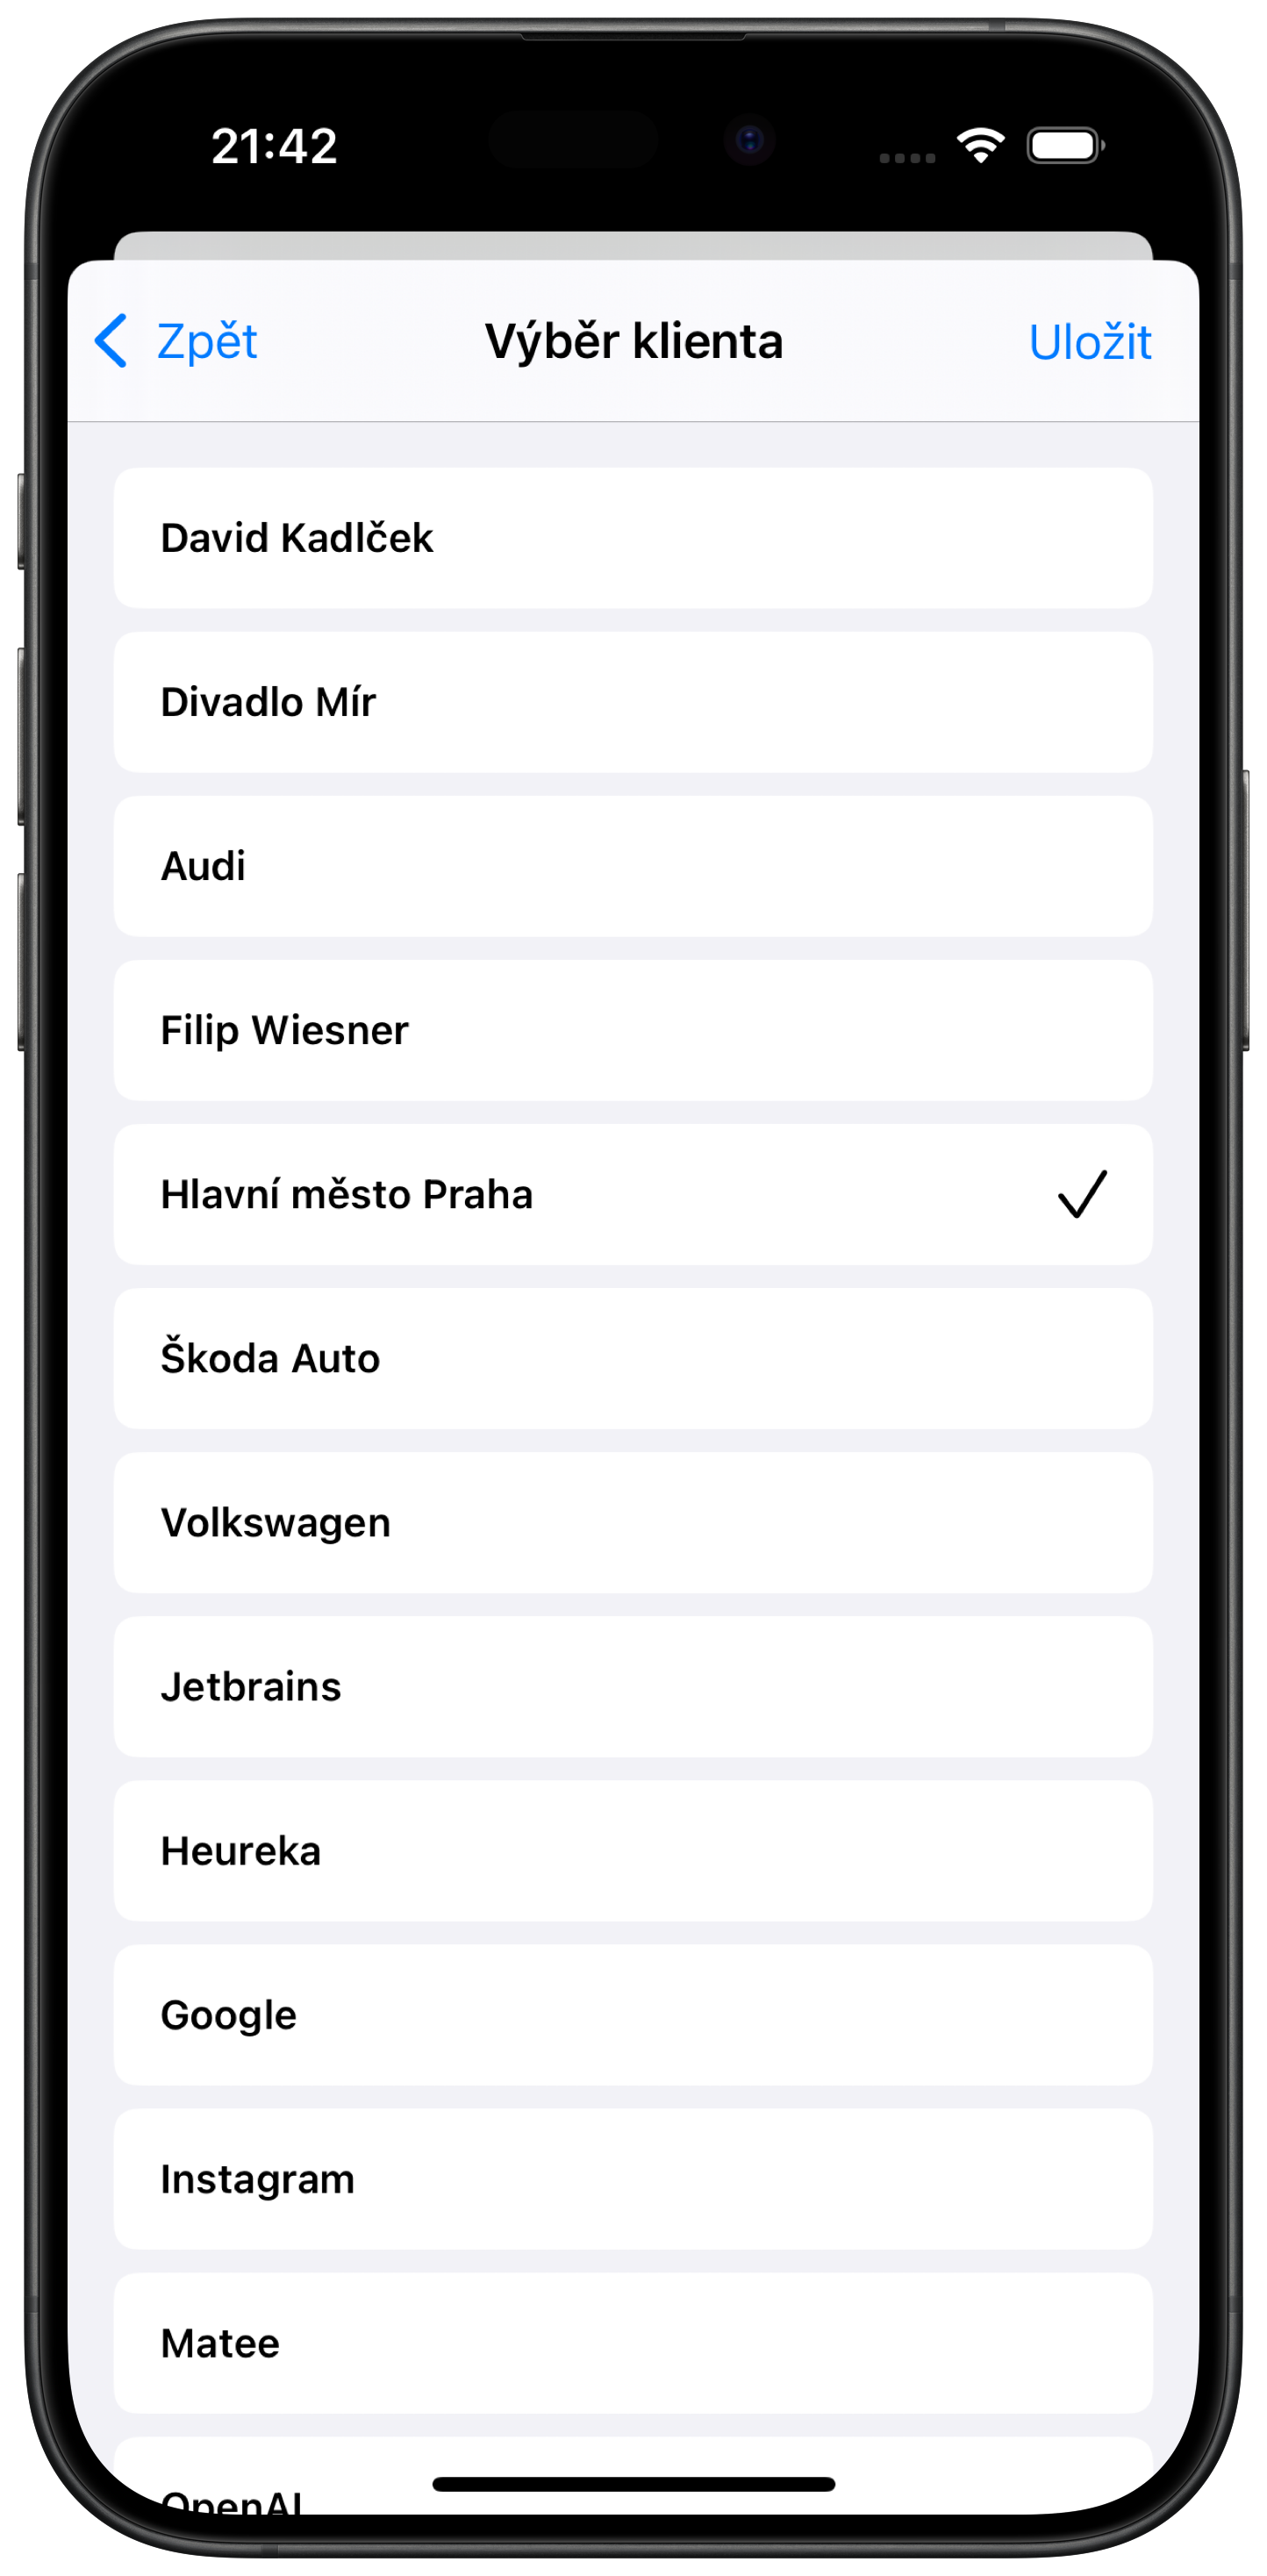
\includegraphics[width=6cm]{client-selection-impl.png}
		\caption{Výběr klienta k~projektu}
		\label{fig:client-selection-impl}
	\end{subfigure}
	\caption{Seznam projektů a~výběr klienta k~projektu}
	\label{fig:project-list-client-selection-impl}
\end{figure}

%---------------------------------------------------------------
\subsection{Integrace}
%---------------------------------------------------------------

Tato funkcionalita pokrývá možnosti, jak může uživatel napojovat aplikaci na navržené spouštěče měření času (import) a~jak propojit aplikaci s~existujícími systémy (export), jak bylo navrženo v~sekci \ref{feature-integration}.

%---------------------------------------------------------------
\subsubsection{Backend}
%---------------------------------------------------------------

Aplikace uživateli umožňuje si nastavené integrace vytvářet, ukládat, upravovat a~mazat. Backend bude tedy muset opět implementovat všechny CRUD operace a~získání všech integrací daného uživatele, tentokrát pro objekty integrací. Toto je odpovědností \texttt{IntegrationRepository} a~jejího \emph{Source}. Na rozdíl od uživatelů, klientů nebo projektů, nejsou integrace propojeny s~jinými typy objektů napříč celou databází, jejich úprava je tedy poměrně jednoduchá a~týká se jen vlastních objektů.

Co se týče exportu do CSV souboru, tak celou tuto logiku implementuje backend, který CSV soubor vytvoří a~klientovi ho pošle hotový. Ve výpisu kódu \ref{code:be-route-csv} lze nahlédnout implementace \emph{Route} pro export do CSV souboru, kde lze vidět, že nejprve získá všechny záznamy v~zadaném období, ty uloží do dočasného lokálního souboru, který pošle klientovi, a~poté dočasný soubor smaže.

\begin{listing}
\caption{\emph{Route} pro export do CSV souboru}\label{code:be-route-csv}
\begin{minted}{Kotlin}
fun Routing.integrationRoute() {

    // ...
    
    authenticate {
        route("/integrations") {
        
            // ...
            
            route("/csv") {
                get {
                    val user = call.requireUserPrincipal().user
                    val from = call.request.queryParameters["from"]
                    val to = call.request.queryParameters["to"]

                    val entries = userRepository.readEntryPreviews(
                        uid = user.uid,
                        startAfter = to?.toInstant(),
                        limit = null,
                        endAt = from?.toInstant()
                    ).data
                    val csv = repository.readCsv(entries.reversed())

                    call.respondFile(csv)

                    repository.deleteTempCsvFile(csv.name)
                }
            }
            
            // ...
        }
    }
}       
\end{minted}
\end{listing}

Napojení aplikace na spouštěče měření (import), které byly pro aplikaci Trackee navrženy, je záležitostí klienta, jelikož se jedná o~systémovou aplikaci \emph{Zkratky}. Bude pouze potřeba poskytnout dodatečné API, které umožní samotné zapnutí časovače, jeho zrušení a~jeho vypnutí spolu s~vytvořením nového časového záznamu. Tyto funkce totiž pro potřeby funkcionality časovače implementuje klientská aplikace ručně, která aktualizuje aktuální nastavení časovače, čímž reálně ovlivňuje to, zda časovač běží, od kdy běží, a~podobně. Při tvorbě nového záznamu také volá pouze API pro ruční vytvoření nového záznamu, protože všechna potřebná data zná. Při použití zkratek se jedná pouze o~jednoduchý požadavek, který ale nemá žádné informace o~aktuálním nastavení časovače, takže pro tyto potřeby bude tato logika na backendu. Alternativou by bylo, aby vyvolané \emph{Zkratky} přímo interagovaly s~rozhraním aplikace, ale to by nedávalo moc smysl, protože v~tomto případě je tím rozhraním právě aplikace \emph{Zkratky}.

%---------------------------------------------------------------
\subsubsection{Multi-platformní část}
%---------------------------------------------------------------

Multi-platformní část pokrývá funkcionalitu integrací ve dvou modulech – \texttt{integration} a~\texttt{intent}. Modul \texttt{integration} pokrývá všechny funkce, které aplikace nabízí v~kartě \emph{Integrace} (návrh z~obrázku \ref{fig:integration-list}), a~modul \texttt{intent} nabízí funkce pro \emph{Intents}, což jsou obsluhy jednotlivých zkratek aplikace \emph{Zkratky}, jak bylo popsáno v~sekci \ref{feature-integration-import}.

Modul \texttt{integration} poskytuje tyto \emph{Use Cases}:
\begin{itemize}
\item\texttt{AddIntegrationUseCase} – Přidá novou integraci.
\item\texttt{DeleteIntegrationUseCase} – Smaže integraci podle jejího identifikátoru.
\item\texttt{ExportToCsvUseCase} – Exportuje data ve zvoleném období do CSV souboru.
\item\texttt{GetIntegrationsUseCase} - Získá všechny integrace přihlášeného uživatele.
\item\texttt{GetIntegrationUseCase} – Získá integraci podle jejího identifikátoru.
\item\texttt{UpdateIntegrationUseCase} – Aktualizuje integraci.
\end{itemize}
Modul \texttt{intent} poté poskytuje následující \emph{Use Cases}:
\begin{itemize}
\item\texttt{CancelTimerUseCase} – Zruší běžící časovač, zahodí tedy jeho data. Pokud časovač neběží, neudělá nic.
\item\texttt{StartTimerUseCase} – Spustí časovač, tedy aktualizuje jeho data tak, že bude ve stavu \texttt{active} a~bude měřit od momentu, kdy byl \emph{Use Case} zavolán. Pokud časovač už běží, neudělá nic (tedy počátek měření zůstane nezměněn).
\item\texttt{StopTimerUseCase} – Zastaví časovač a~vytvoří z~jeho dat nový časový záznam. Pokud například chybí zadání vybraného projektu, tak \emph{Use Case} vrátí chybu. Pokud časovač neběží, neudělá nic.
\end{itemize}
U~těchto \emph{Use Cases} je důležité, aby v~případě, že se daný \emph{Intent} snaží dostat časovač do stavu, ve kterém již je, opravdu neudělal nic. Tedy například v~případě opakovaného zapnutí nebyl měněn čas zapnutí podle nového volání. Je tak potřeba proto, protože operace zkratek jsou navrženy tak, aby byly idempotentní\footnote{Operace je idempotentní, pokud jejím opakovaným použitím na nějaký vstup vznikne stejný výstup, jako vznikne jediným použitím dané operace. \cite{idempotence}}. Tyto zkratky totiž pravděpodobně budou součástí nějakých automatizací, které můžou například zapínat časovač podle polohy. Pokud by opakované spuštění zkratky přepisovalo data podlé nových informací, byla by původní data smazána a~uživatel by o~ně přišel. Podnětem pro budoucí vylepšení aplikace může být například to, aby se v~případě, že uživatel vyvolá zkratku pro spuštění časovače s~novými daty, když už časovač běží, časovač automaticky zastavil, uložil nový časový záznam z~dosud běžících dat, a~poté se znovu zapnul pro nová data.

%---------------------------------------------------------------
\subsubsection{Nativní aplikace}
%---------------------------------------------------------------

Uživatelské rozhraní iOS aplikace dodržuje návrh ze sekce \ref{feature-integration}. Na obrázku \ref{fig:integrations-empty-impl} lze vidět kartu integrací ve stavu, když uživatel nemá vytvořené žádné integrace. Na obrázku \ref{fig:new-integration-impl} lze poté vidět rozhraní pro tvorbu nové CSV integrace. Export CSV dat a~jejich vizualizace v~aplikaci \emph{Numbers} lze nahlédnout na obrázku \ref{fig:export-csv-impl}. Pro tvorbu zkratek bude sloužit systémová aplikace \emph{Zkratky}, jejíž hlavní stránka lze vidět na obrázku \ref{fig:shortcuts-impl}, rozhraní pro tvorbu nové zkratky lze pak vidět na obrázku \ref{fig:new-shortcut-impl}. Na obrázku \ref{fig:new-trackee-shortcut} lze poté vidět nabídka možností zkratek pro aplikaace Trackee a~možnost nastavení parametrů zkratky. a~nakonec je na obrázku \ref{fig:automations-impl} vidět možnost tvorby automatizací pro operace s~časovačem.

\begin{figure}[p]
    \centering
    \begin{subfigure}[b]{0.4\textwidth}
		\centering
		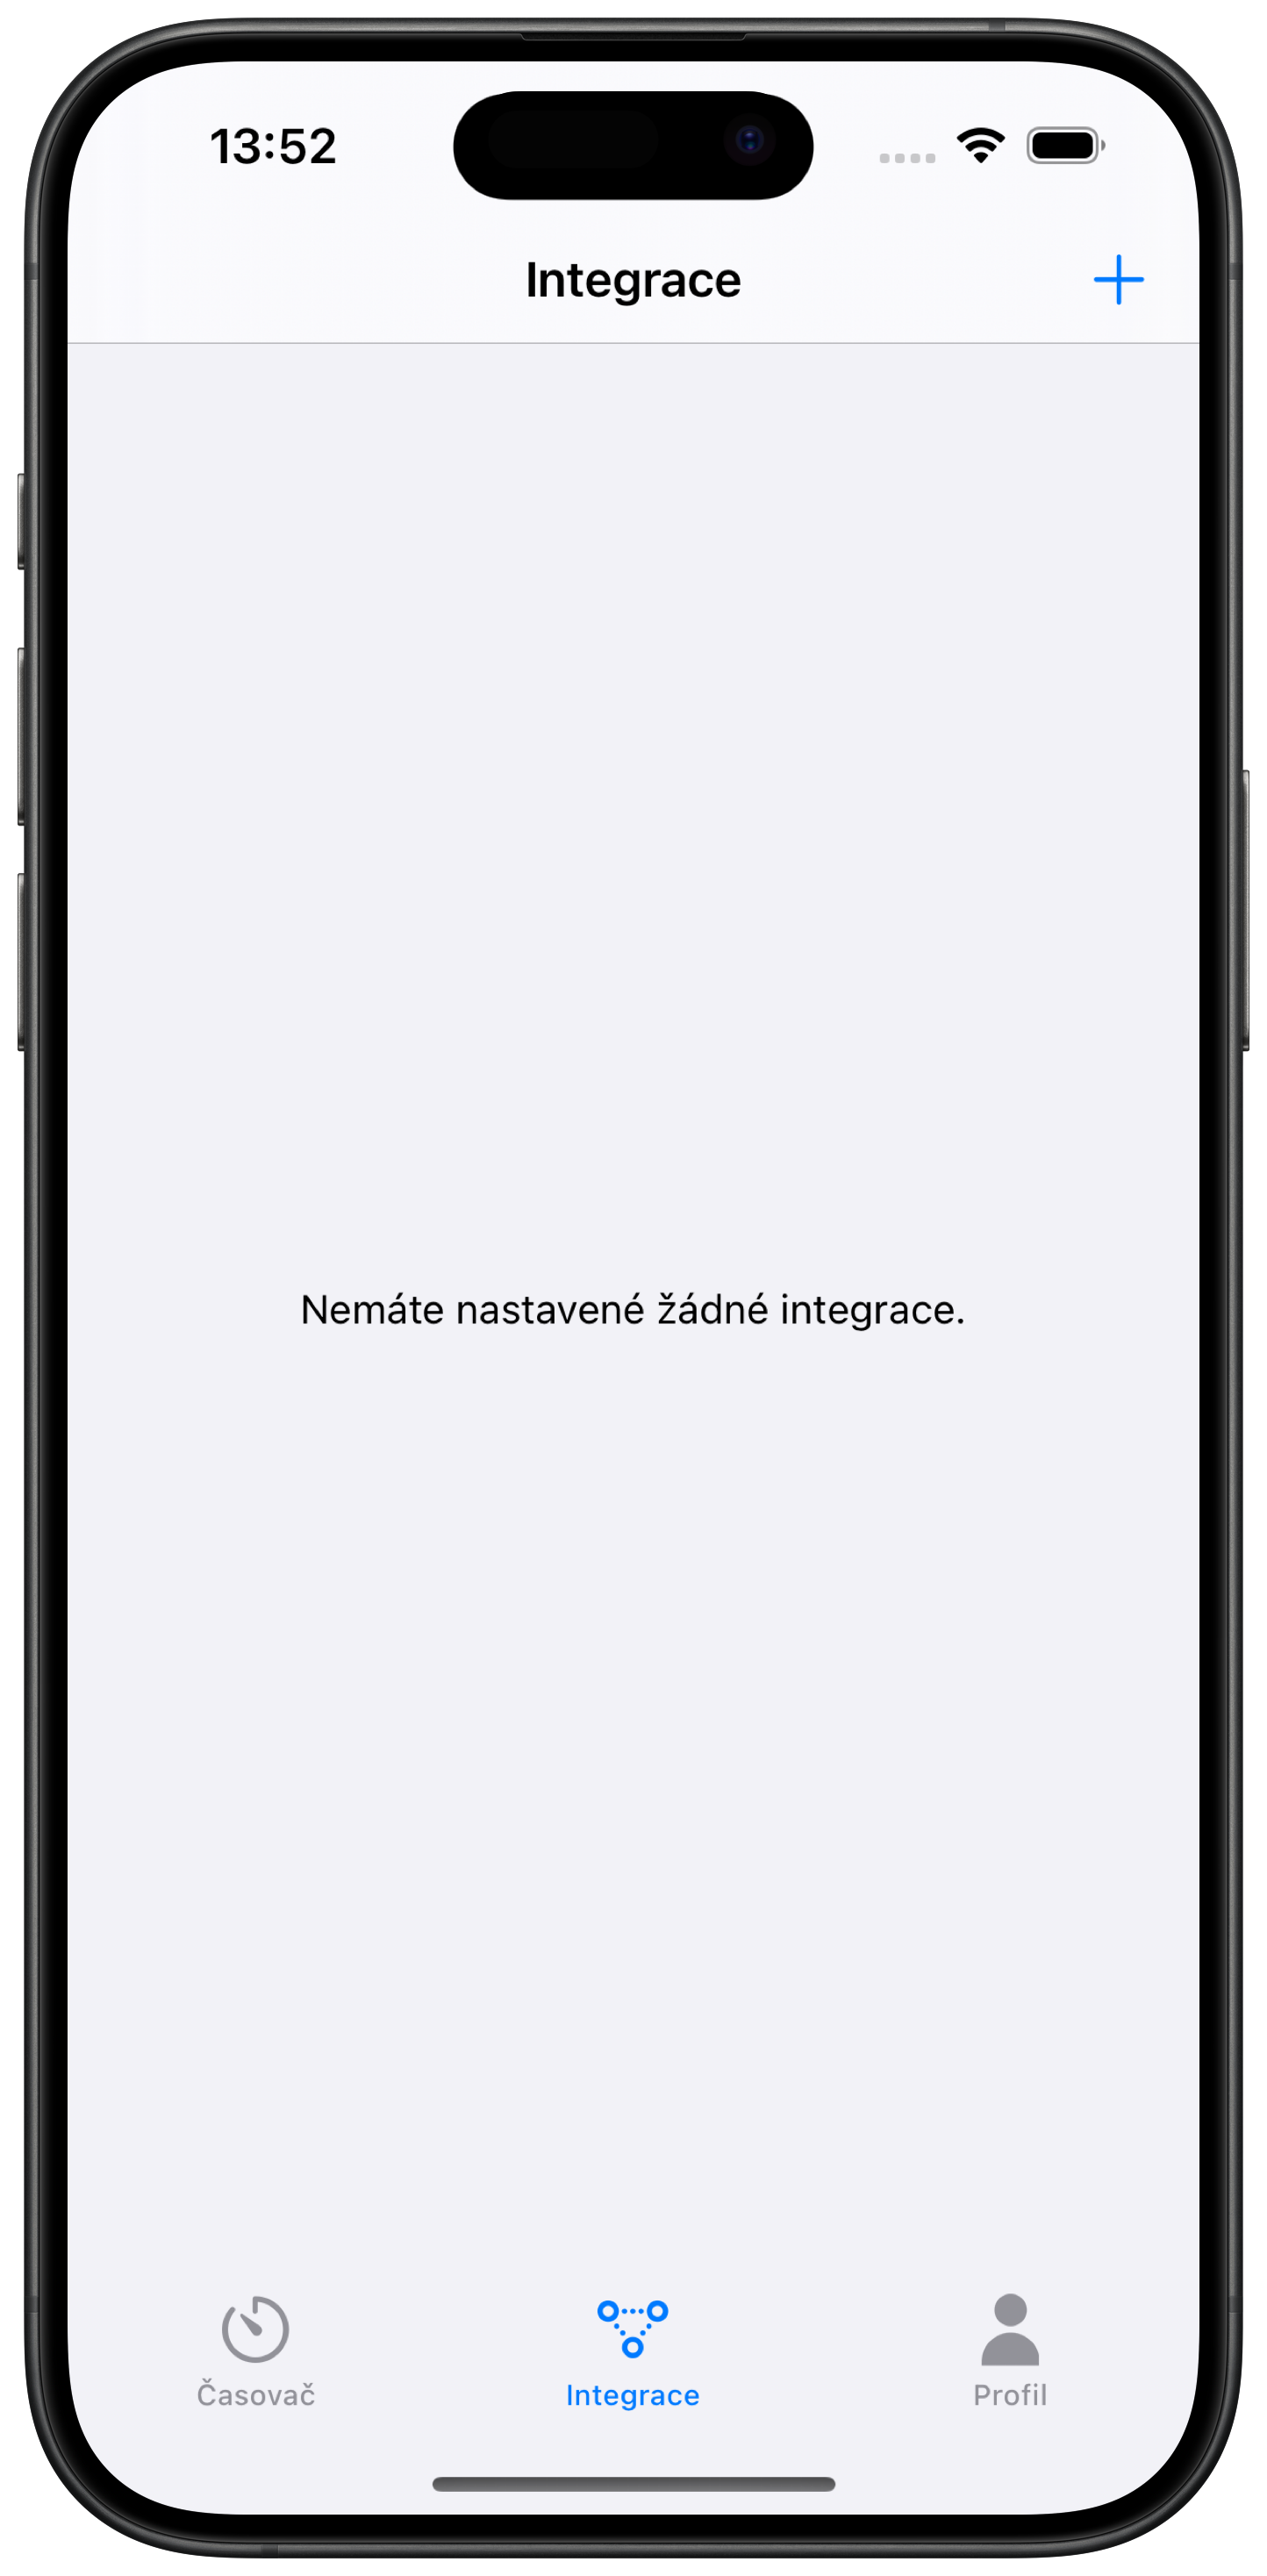
\includegraphics[width=6cm]{integrations-empty-impl.png}
		\caption{Prázdný seznam}
		\label{fig:integrations-empty-impl}
	\end{subfigure}
	\hspace{2cm}
	\begin{subfigure}[b]{0.4\textwidth}
		\centering
		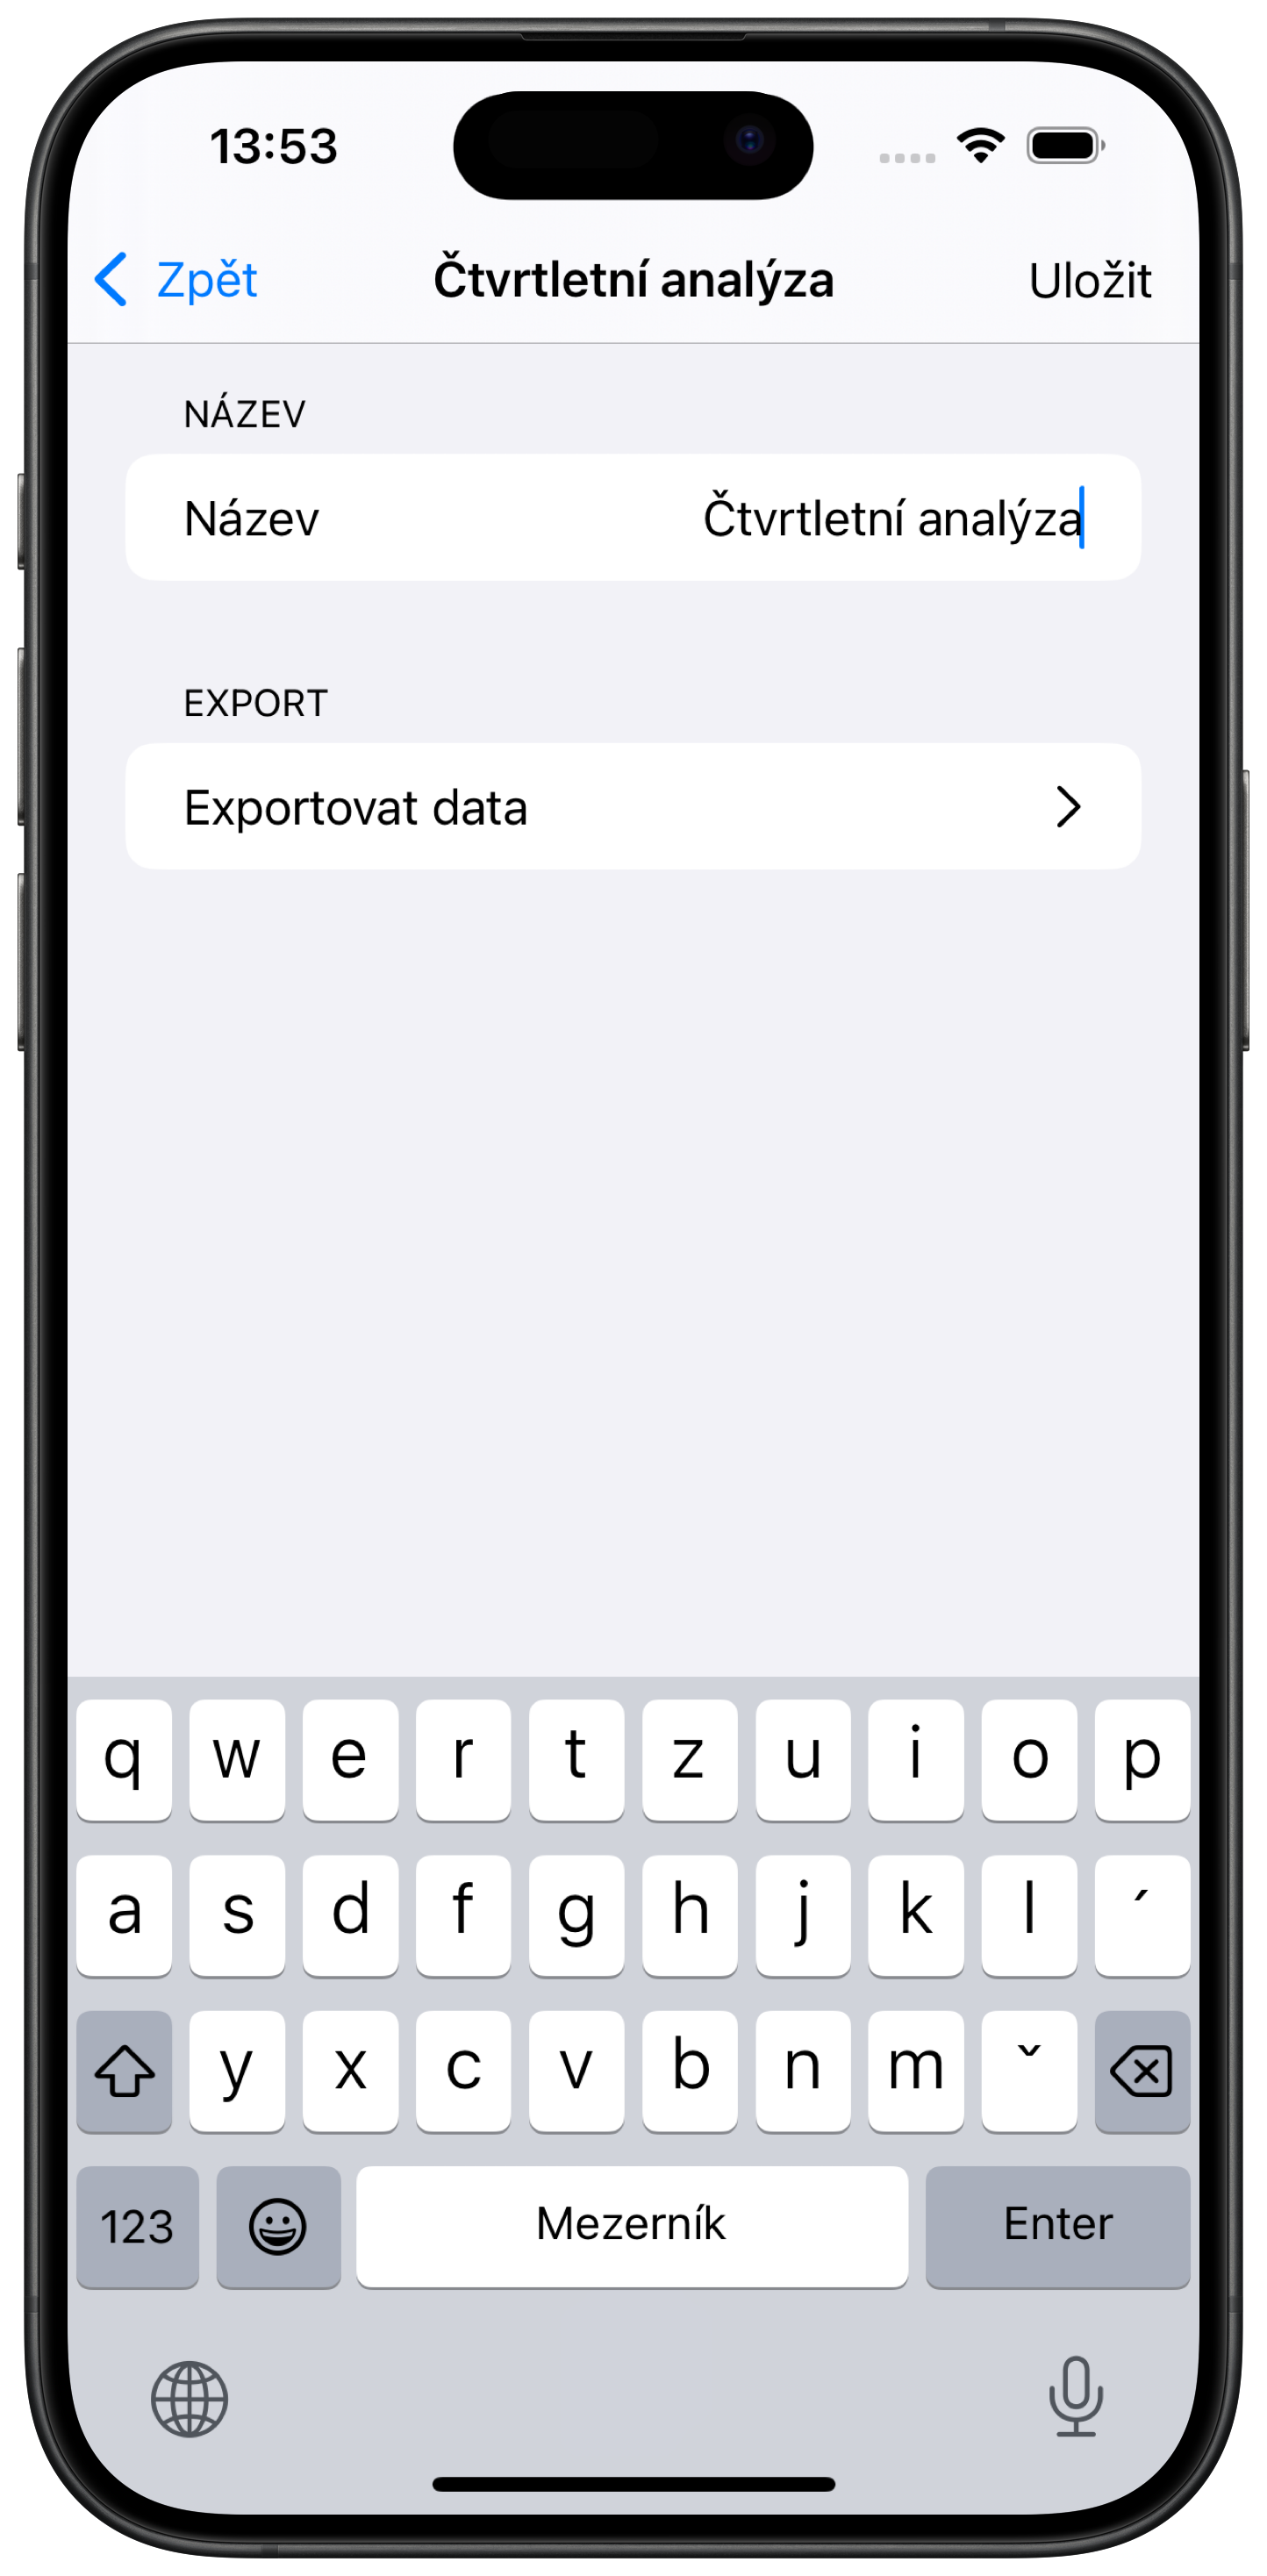
\includegraphics[width=6cm]{new-integration-impl.png}
		\caption{Nová CSV integrace}
		\label{fig:new-integration-impl}
	\end{subfigure}
	\caption{Realizace integrací}
	\label{fig:integrations-impl}
\end{figure}

\begin{figure}[p]
    \centering
    \begin{subfigure}[b]{0.4\textwidth}
		\centering
		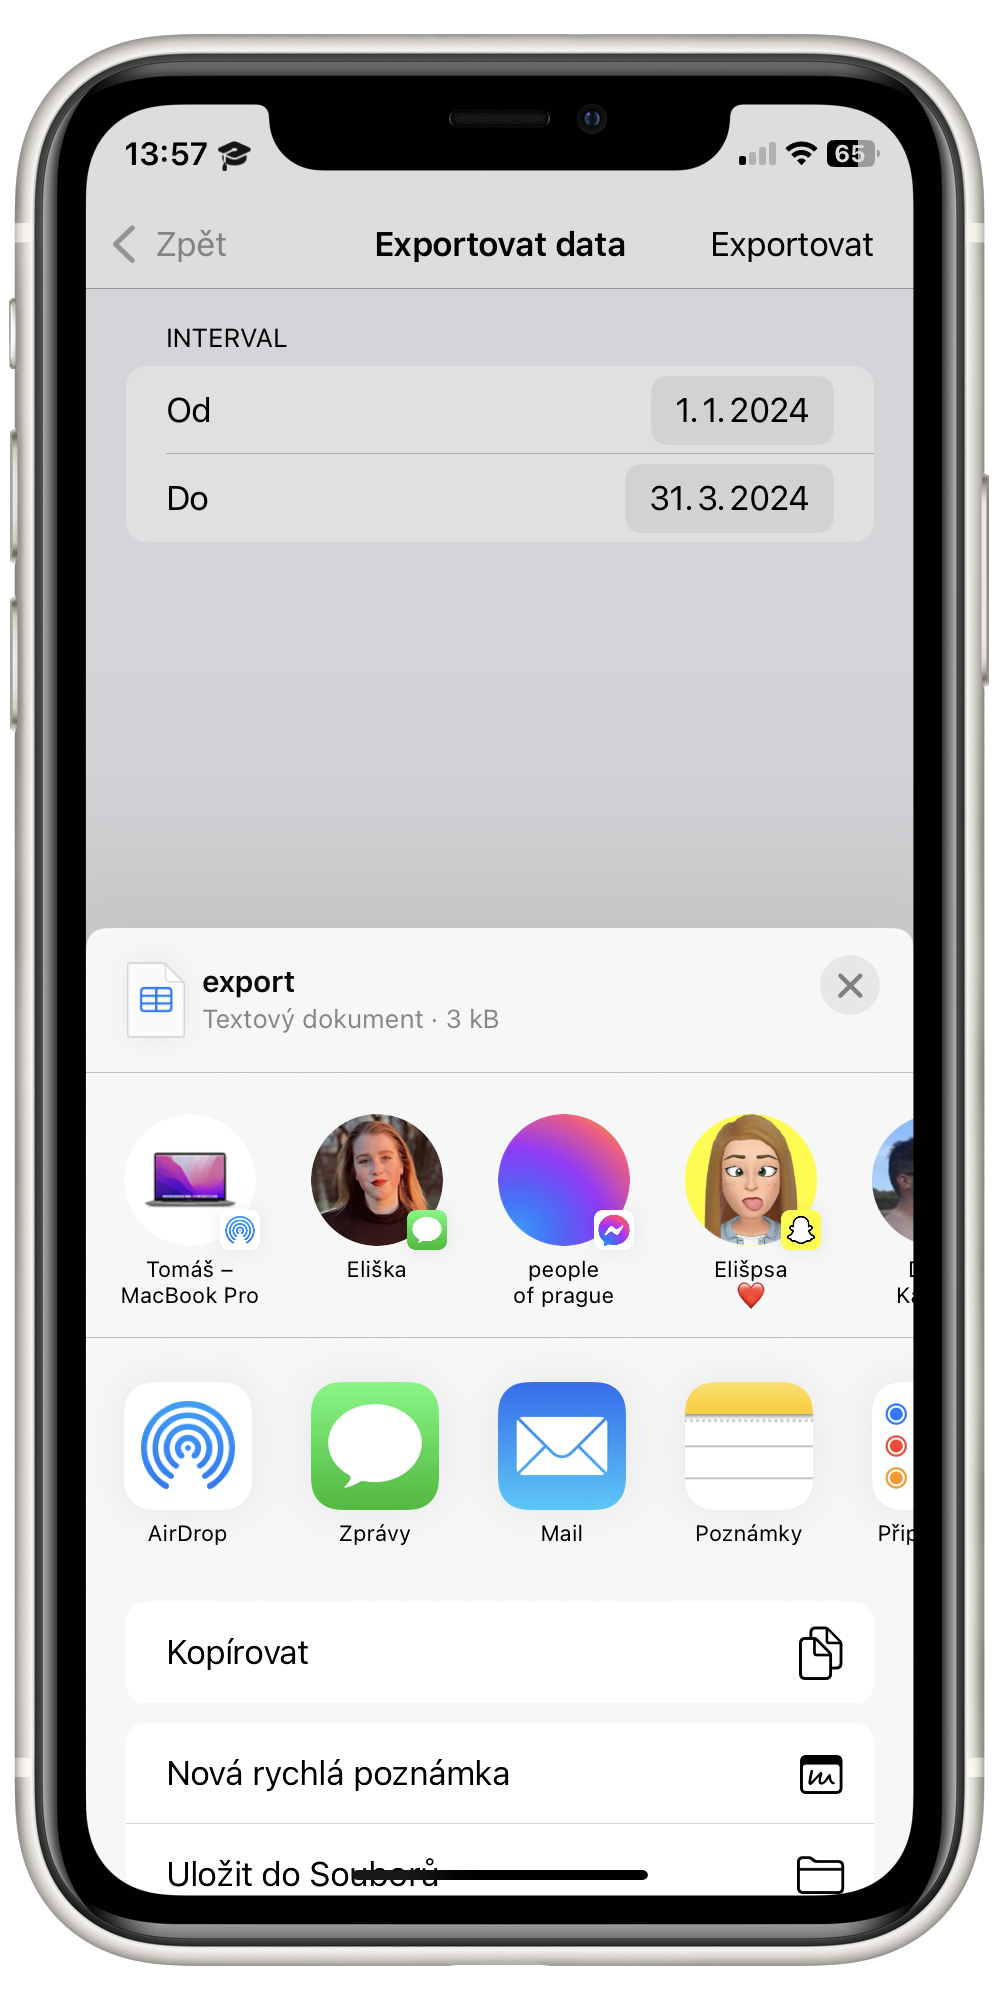
\includegraphics[width=6cm]{export-csv-sheet-impl.png}
		\caption{Dialog pro exportovaný CSV soubor}
		\label{fig:export-csv-sheet-impl}
	\end{subfigure}
	\hspace{2cm}
	\begin{subfigure}[b]{0.4\textwidth}
		\centering
		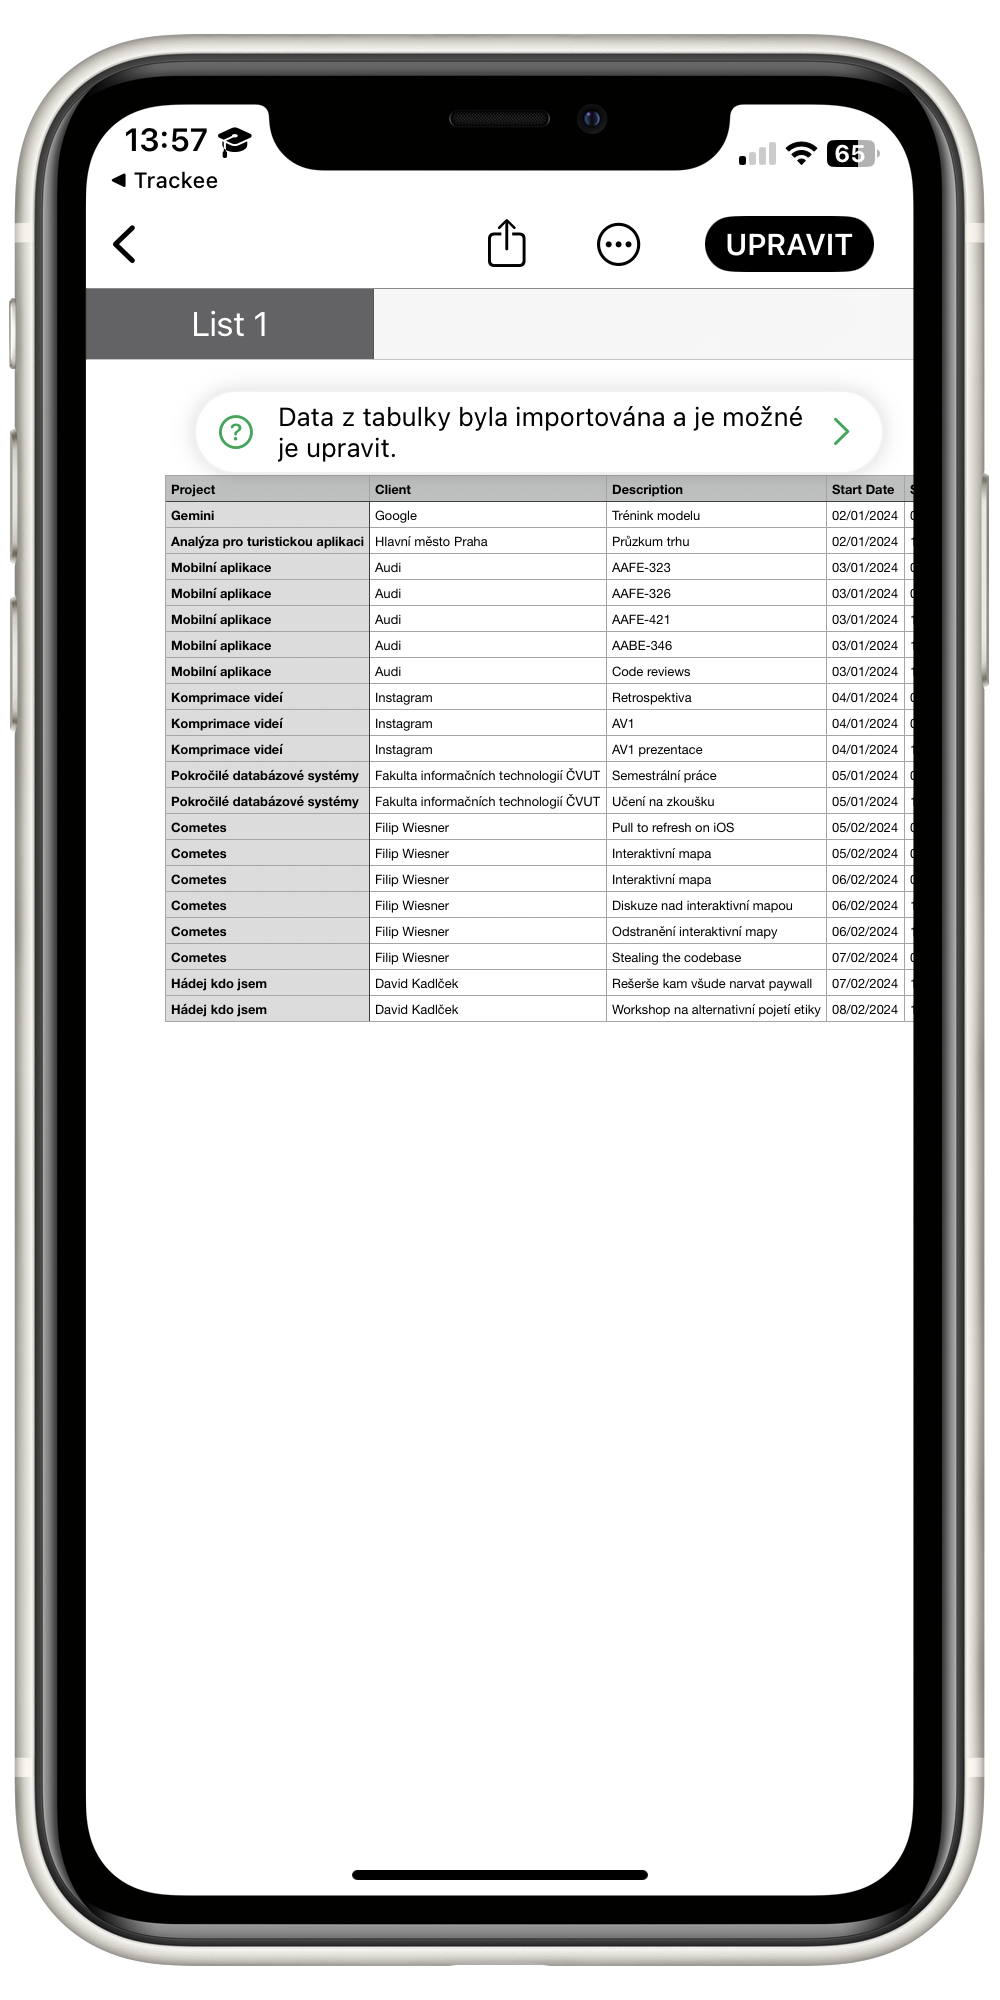
\includegraphics[width=6cm]{export-csv-numbers-impl.png}
		\caption{Exportovaný CSV soubor v~aplikaci \emph{Numbers}}
		\label{fig:export-csv-numbers-impl}
	\end{subfigure}
	\caption{Realizace exportu do CSV}
	\label{fig:export-csv-impl}
\end{figure}

\begin{figure}[p]
    \centering
    \begin{subfigure}[b]{0.4\textwidth}
		\centering
		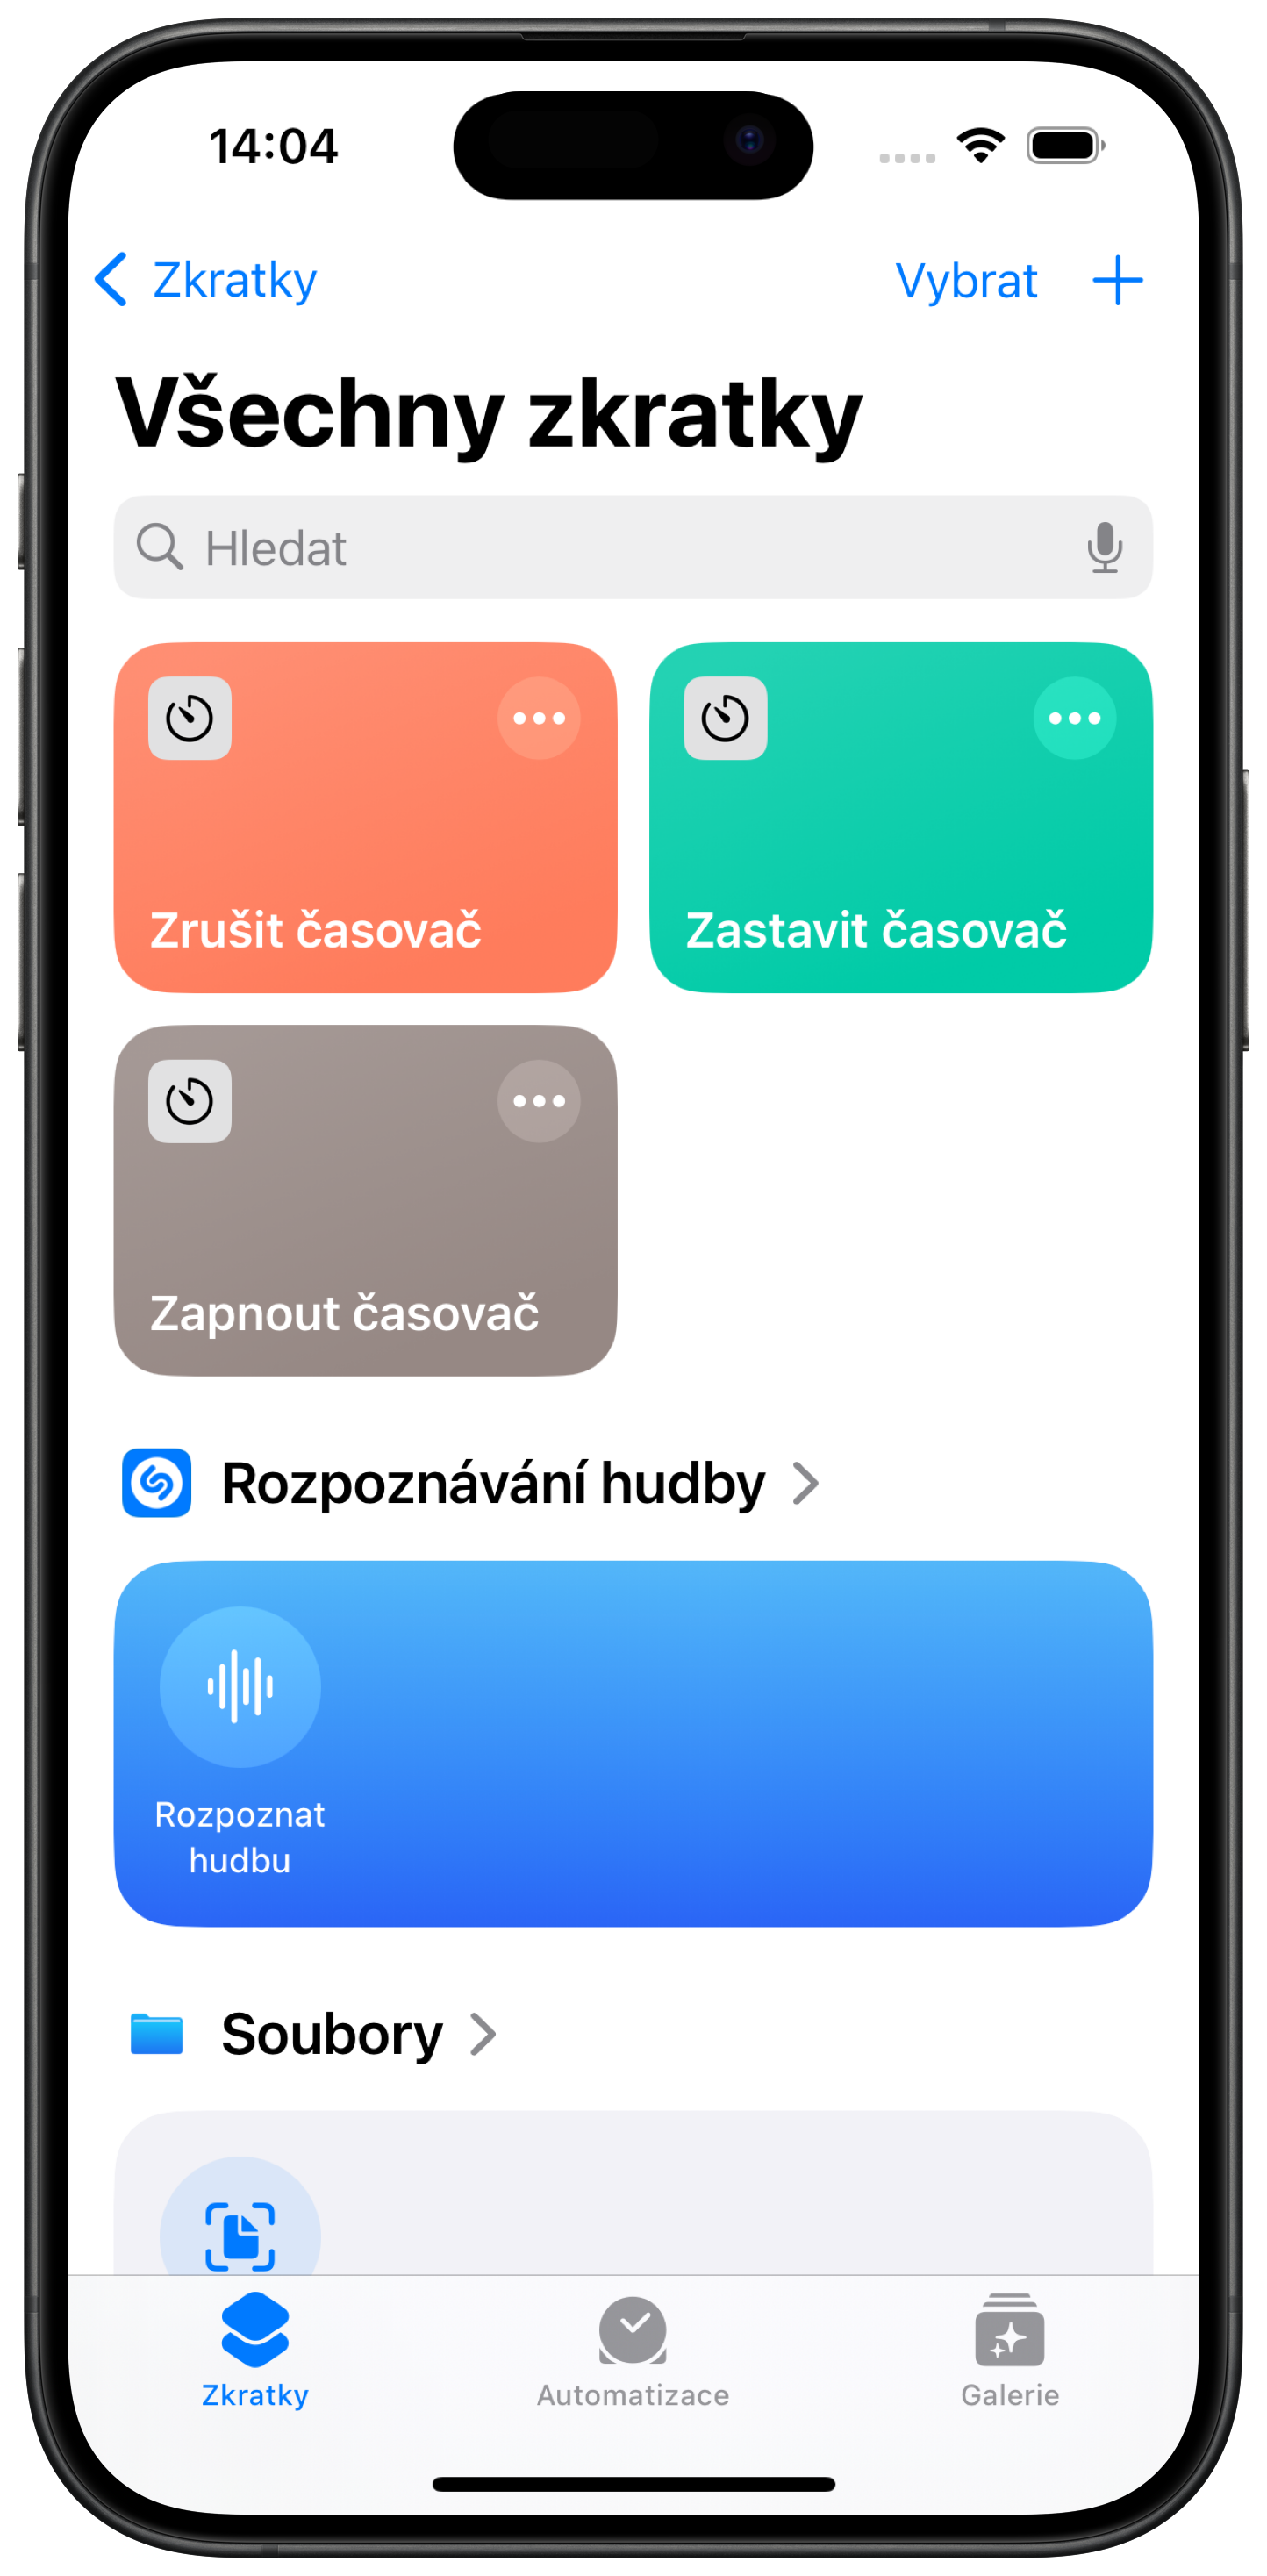
\includegraphics[width=6cm]{shortcuts-impl.png}
		\caption{Přehled zkratek}
		\label{fig:shortcuts-impl}
	\end{subfigure}
	\hspace{2cm}
	\begin{subfigure}[b]{0.4\textwidth}
		\centering
		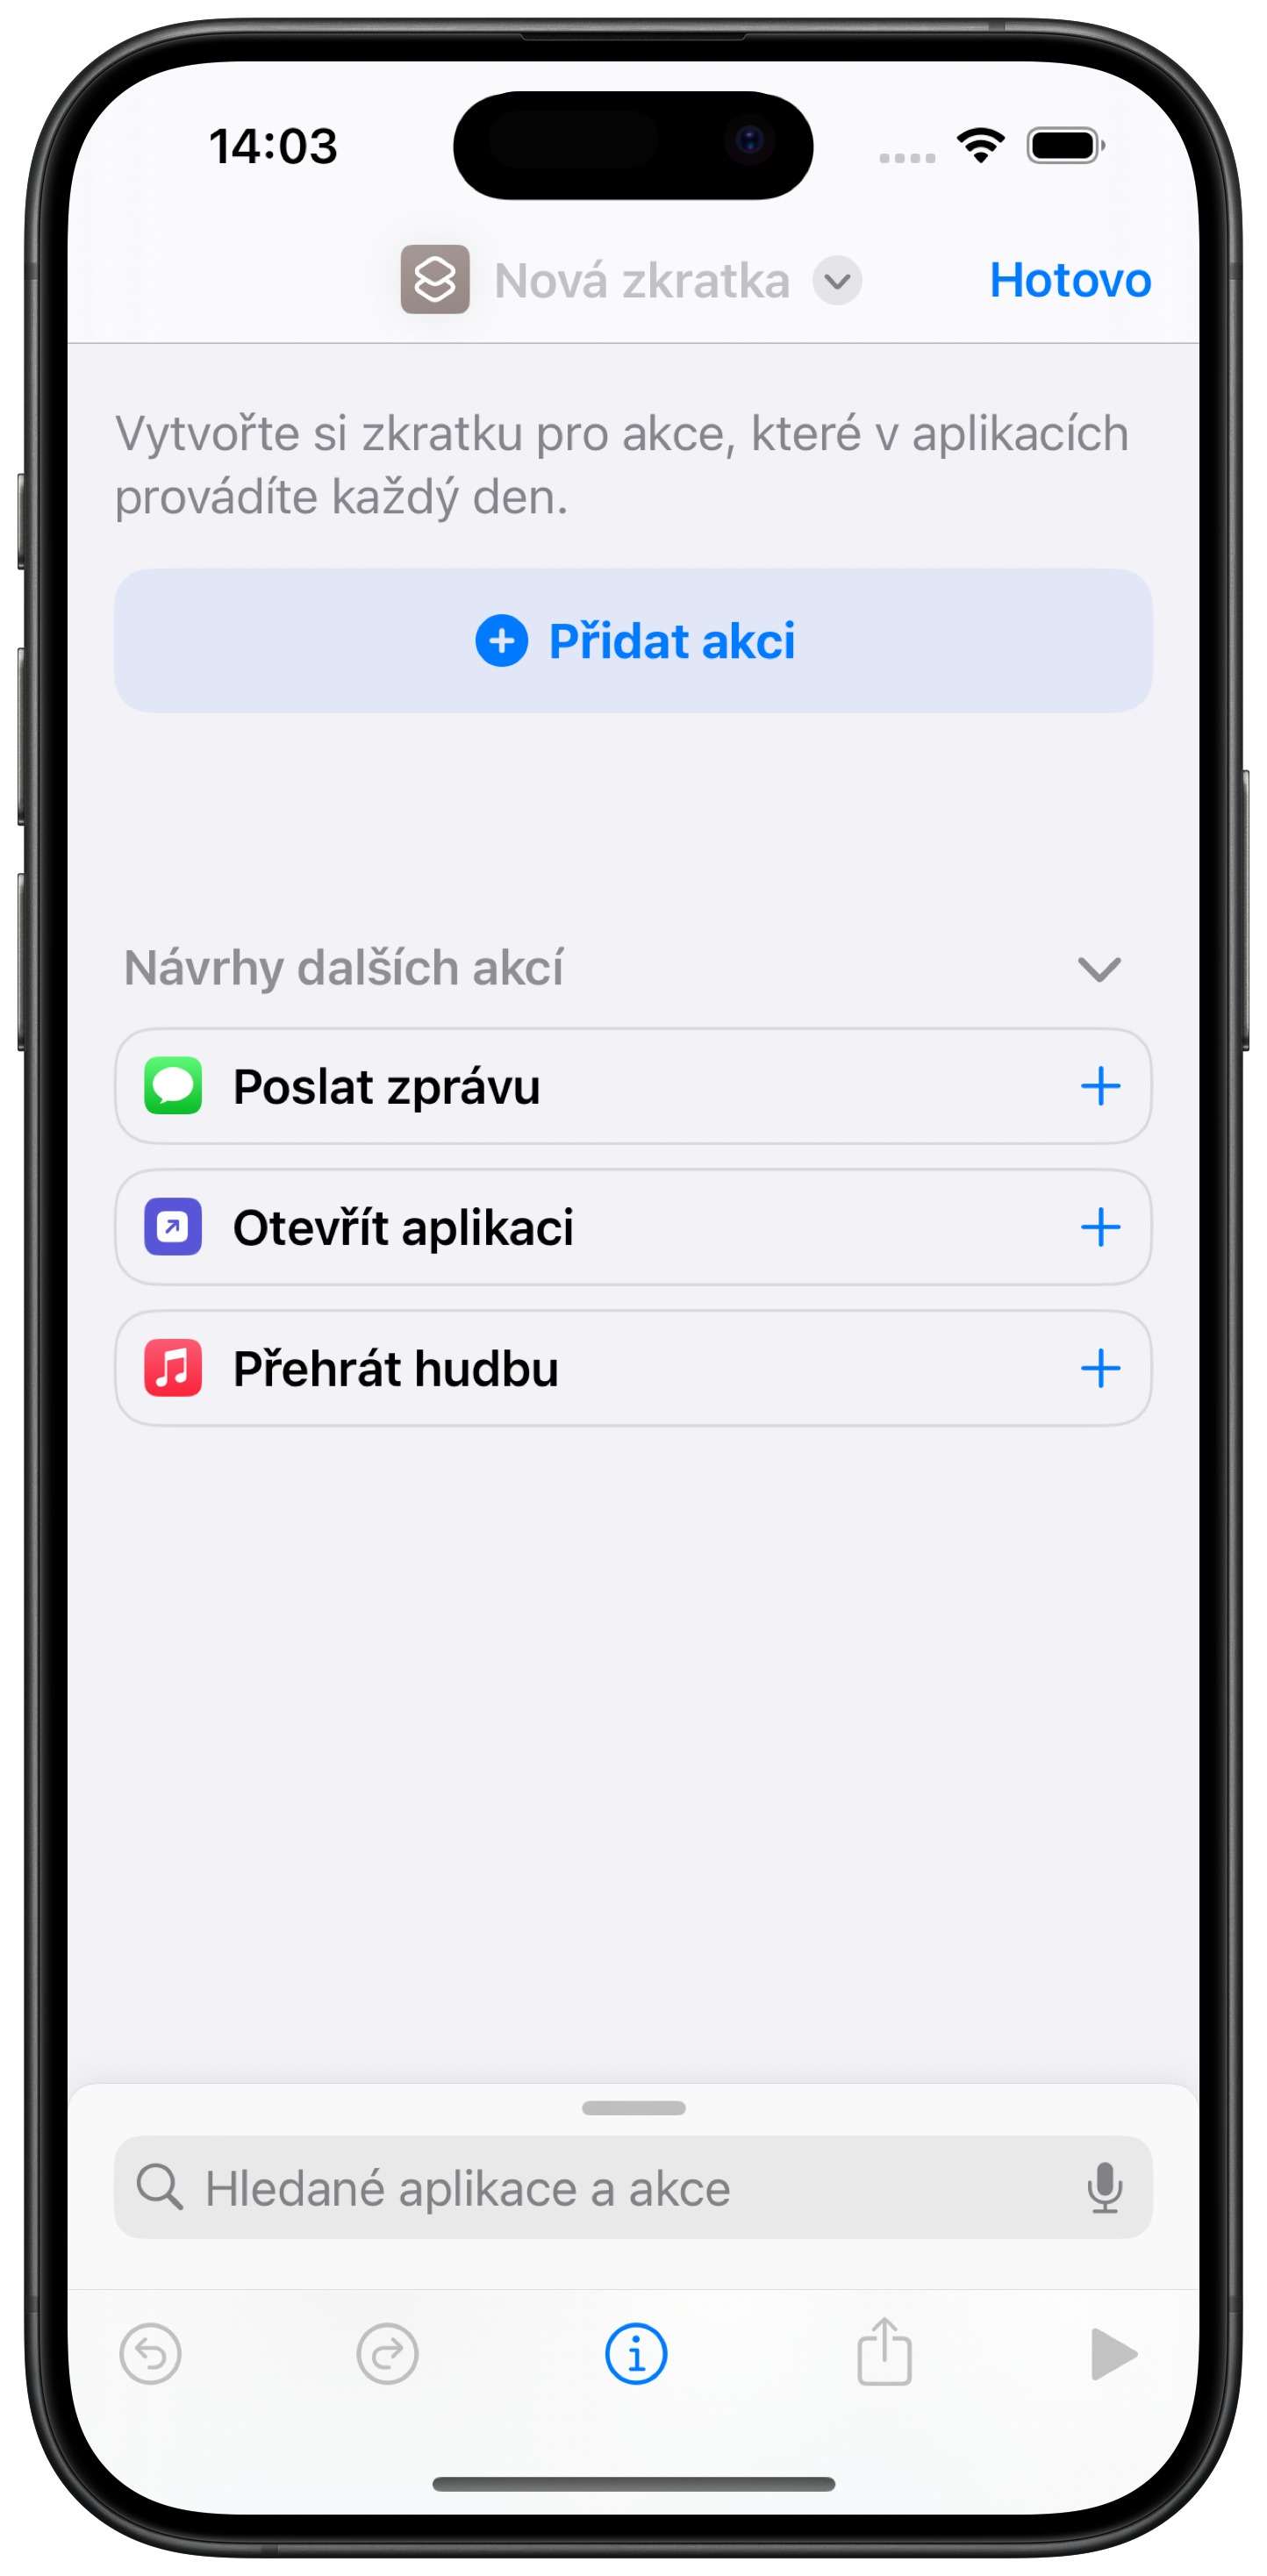
\includegraphics[width=6cm]{new-shortcut-impl.png}
		\caption{Tvorba nové zkratky}
		\label{fig:new-shortcut-impl}
	\end{subfigure}
	\caption{Systémová aplikace \emph{Zkratky}}
	\label{fig:system-shortcuts-impl}
\end{figure}

\begin{figure}[p]
    \centering
    \begin{subfigure}[b]{0.4\textwidth}
		\centering
		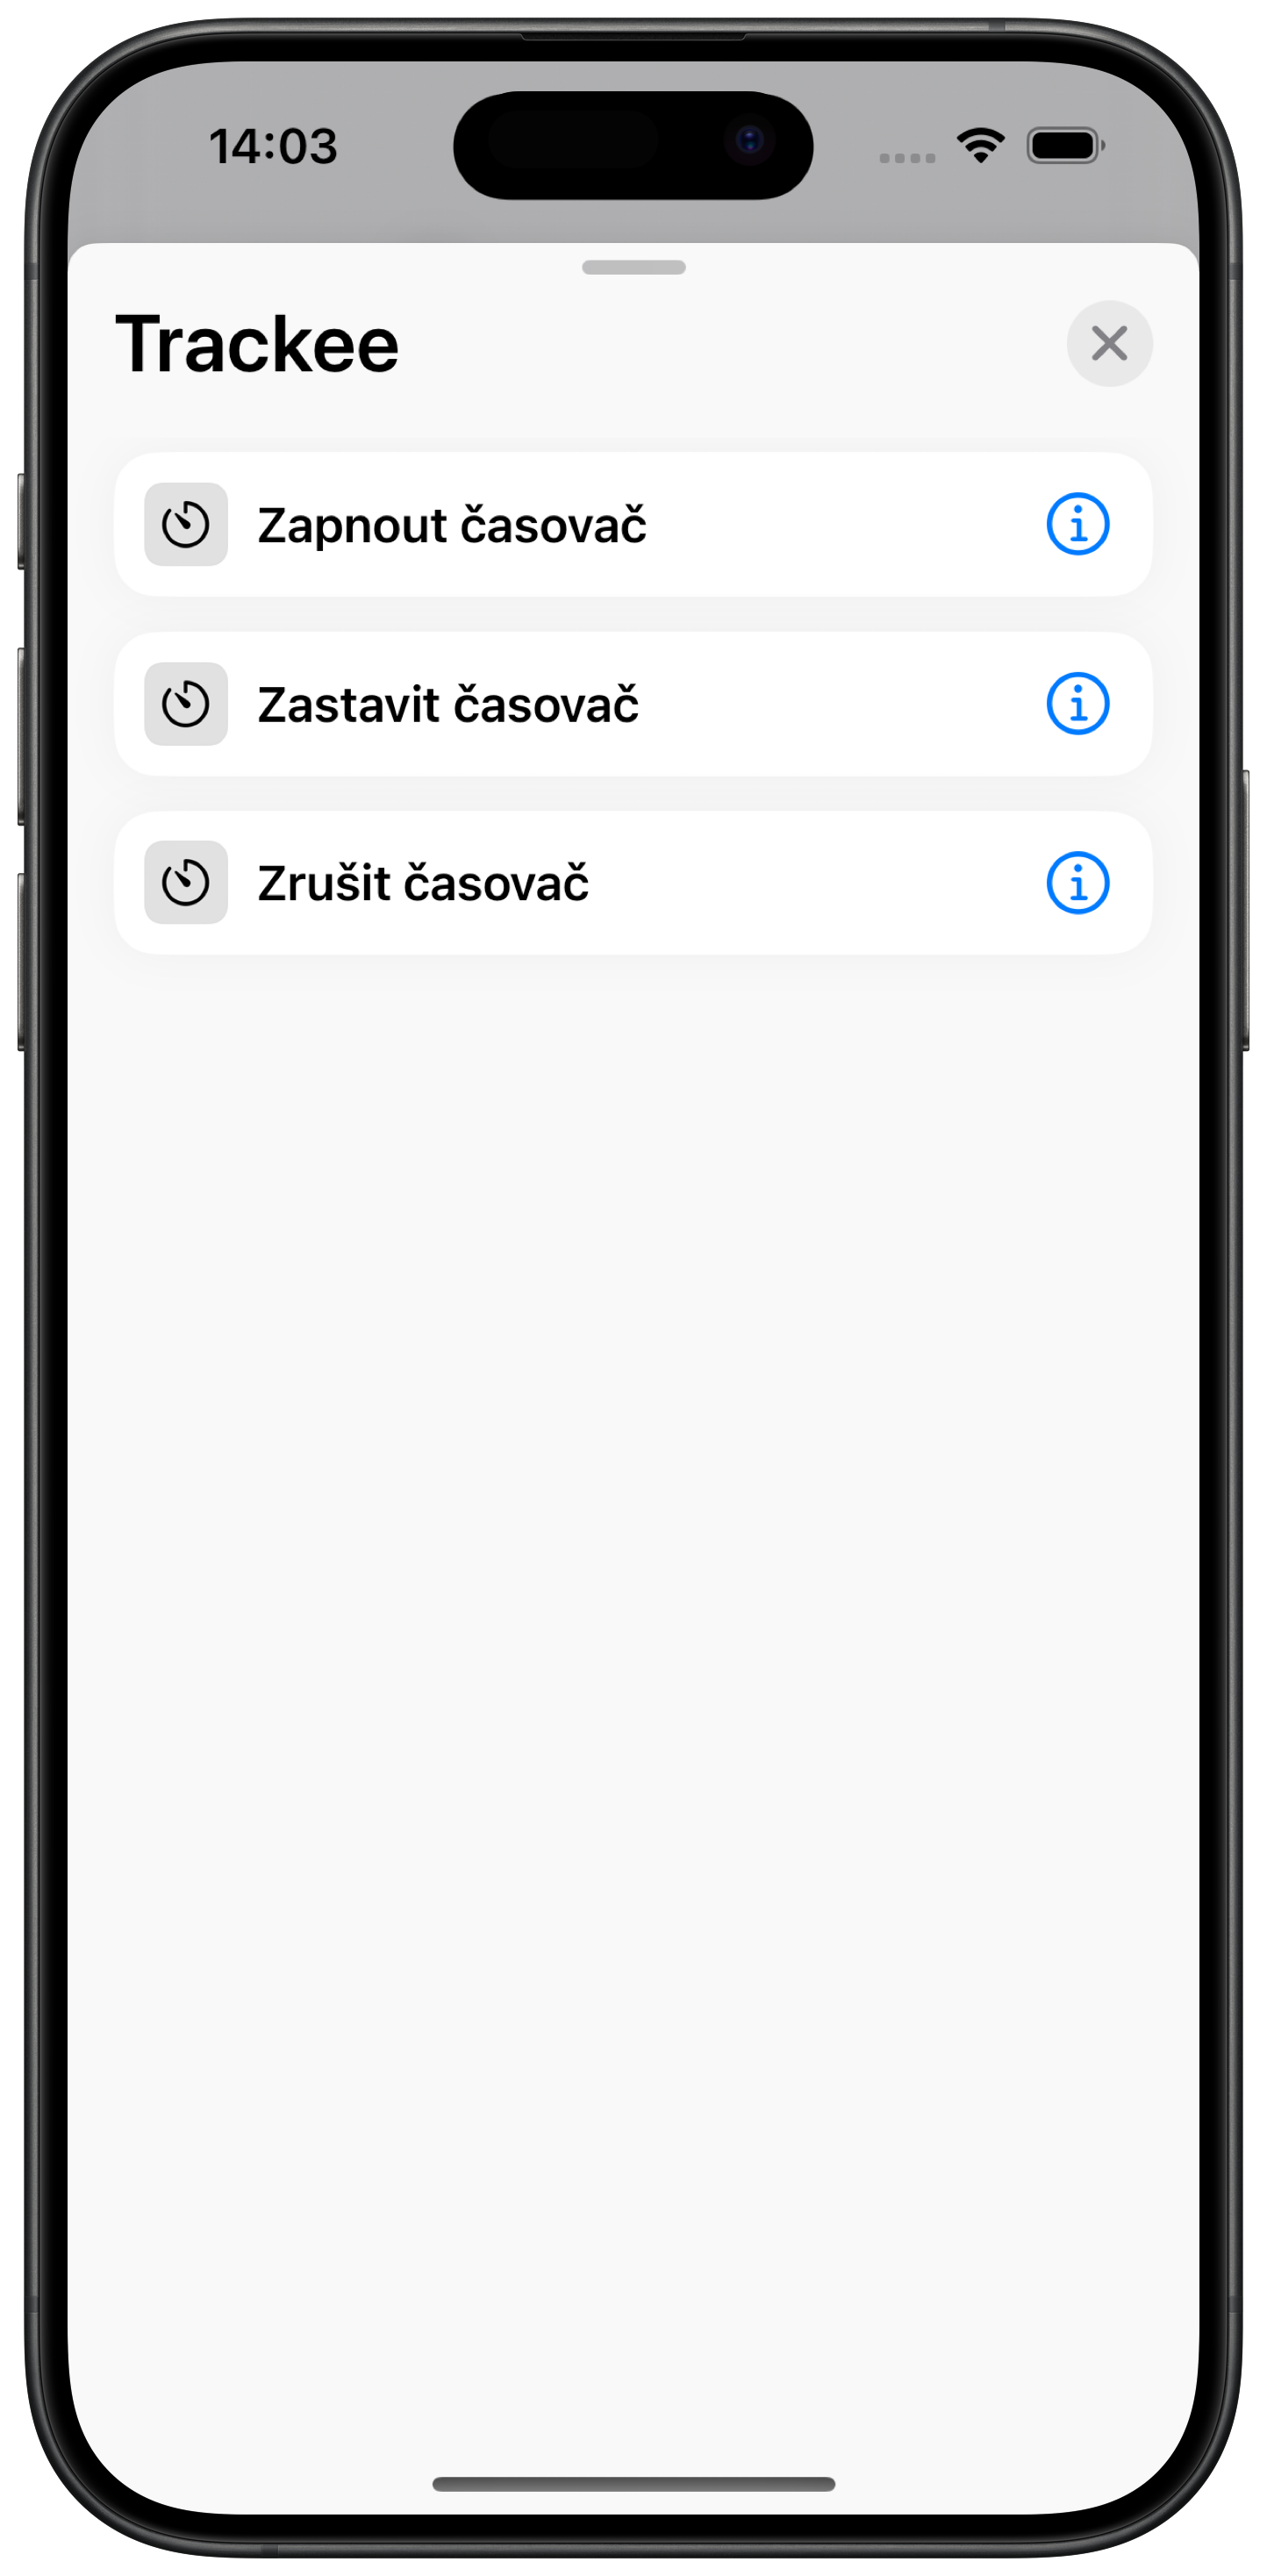
\includegraphics[width=6cm]{new-shortcut-trackee-impl.png}
		\caption{Možnosti zkratek aplikace Trackee}
		\label{fig:new-shortcut-trackee-impl}
	\end{subfigure}
	\hspace{2cm}
	\begin{subfigure}[b]{0.4\textwidth}
		\centering
		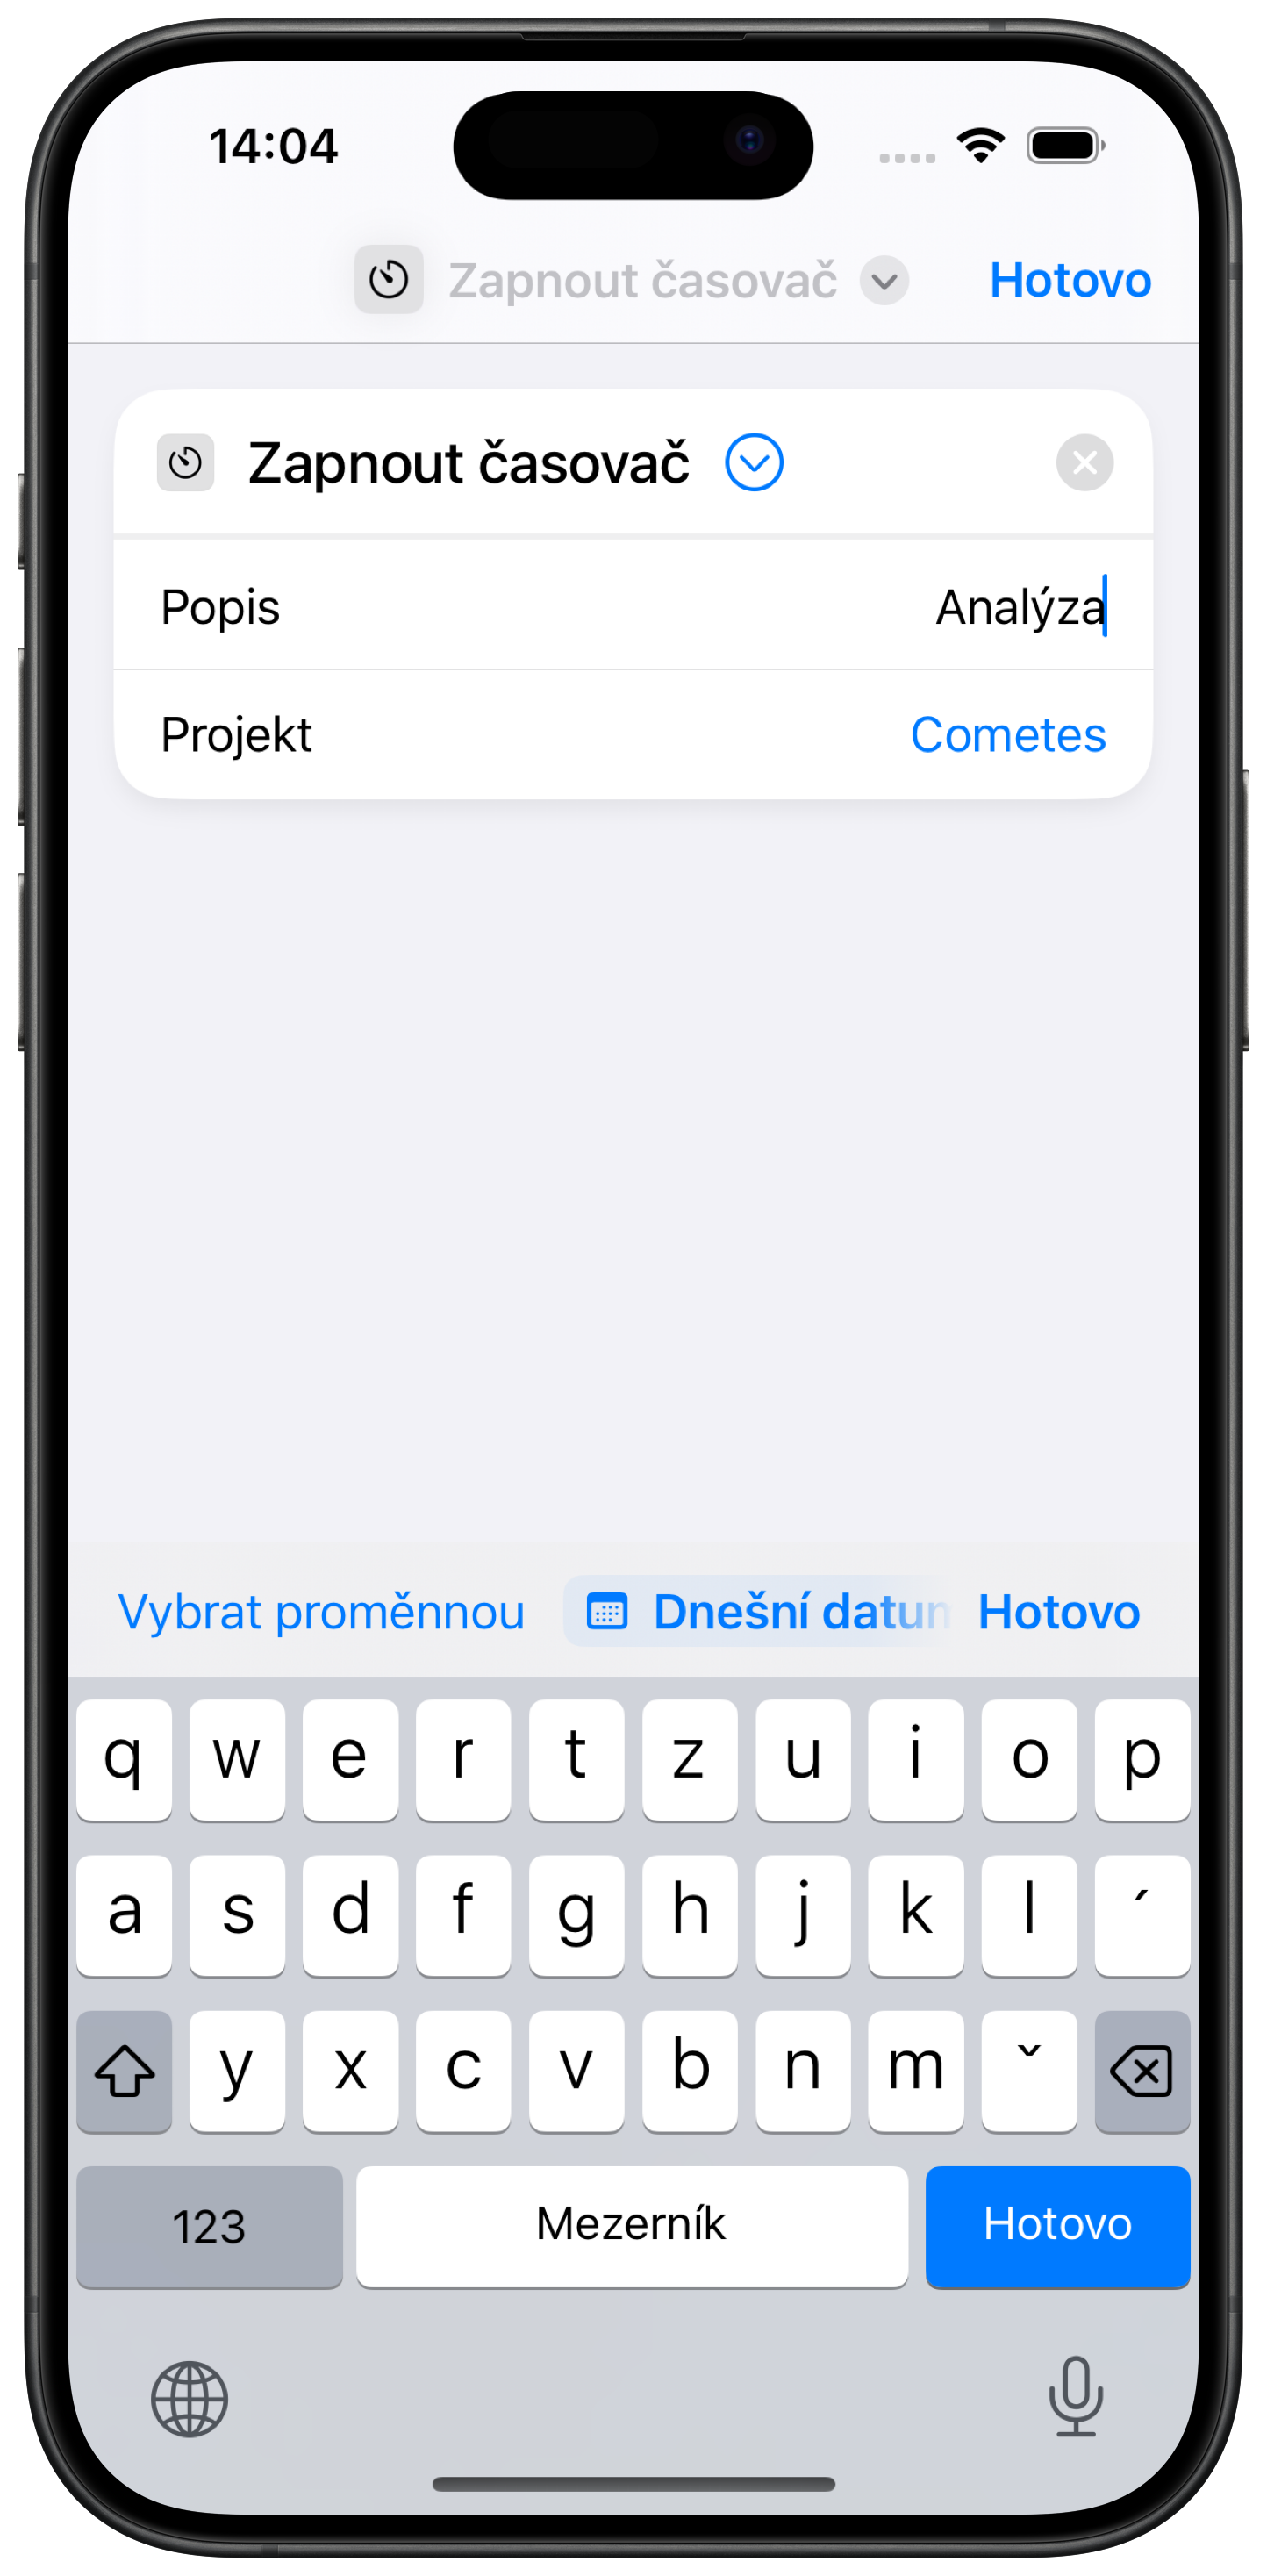
\includegraphics[width=6cm]{new-shortcut-params-impl.png}
		\caption{Parametry zkratky}
		\label{fig:new-shortcut-params-impl}
	\end{subfigure}
	\caption{Tvorba nové zkratky pro Trackee}
	\label{fig:new-trackee-shortcut}
\end{figure}

\begin{figure}[p]
    \centering
    \begin{subfigure}[b]{0.4\textwidth}
		\centering
		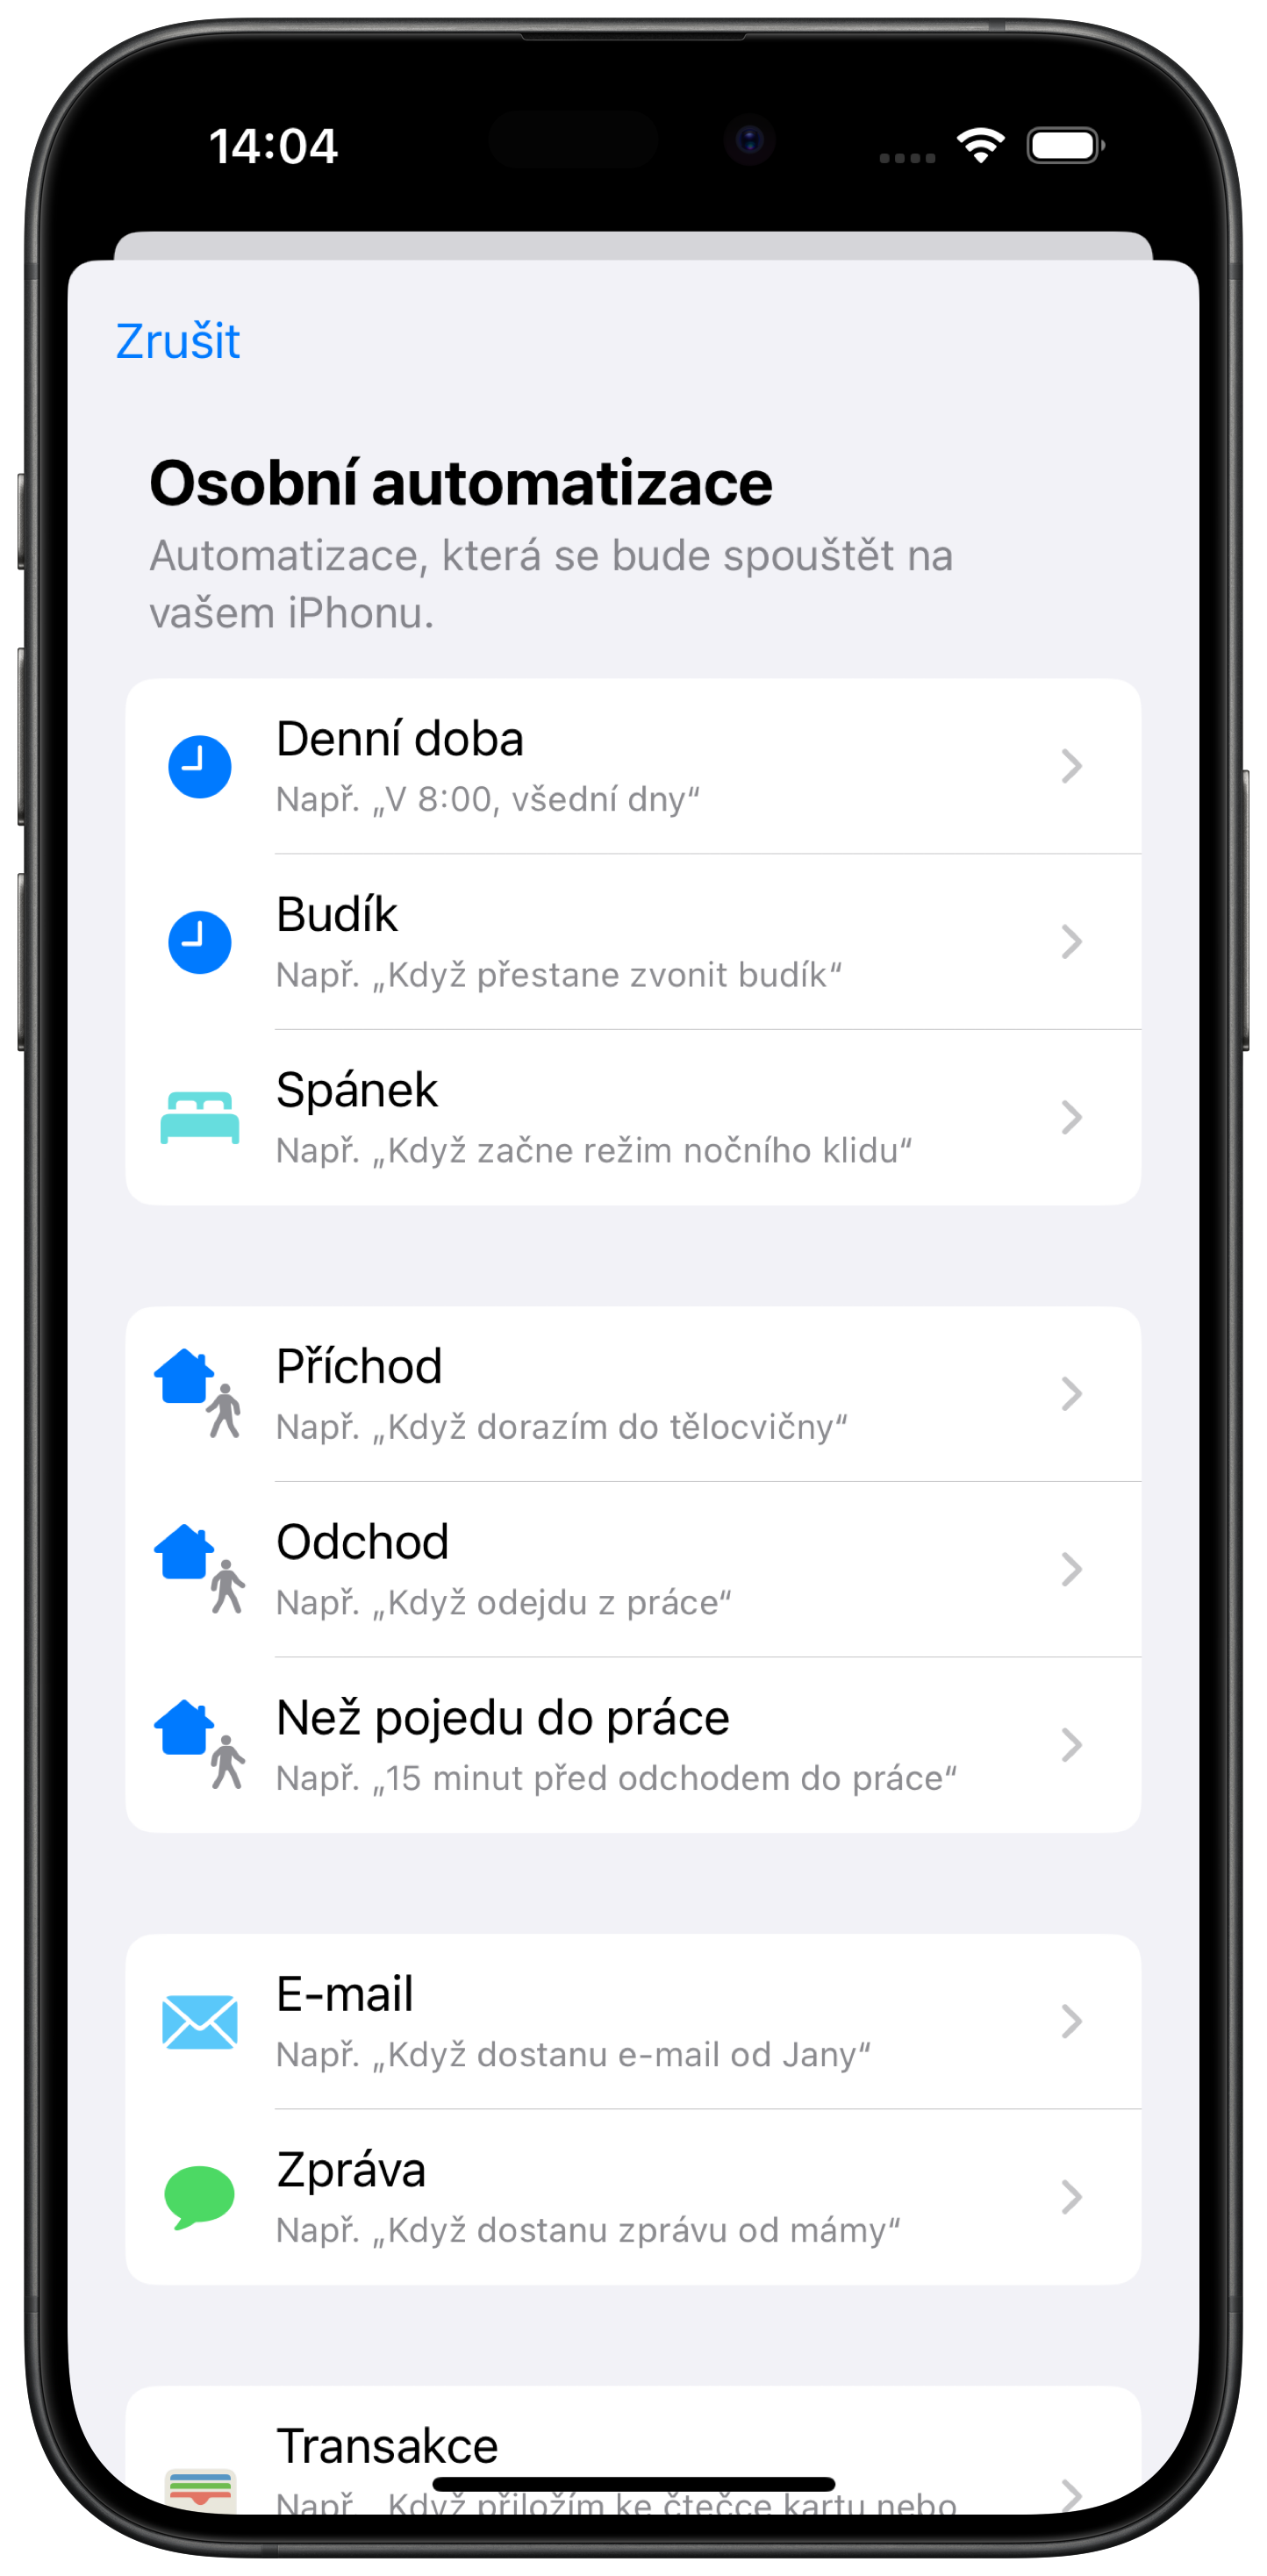
\includegraphics[width=6cm]{new-automation-impl.png}
		\caption{Tvorba nové automatizace}
		\label{fig:new-automation-impl}
	\end{subfigure}
	\hspace{2cm}
	\begin{subfigure}[b]{0.4\textwidth}
		\centering
		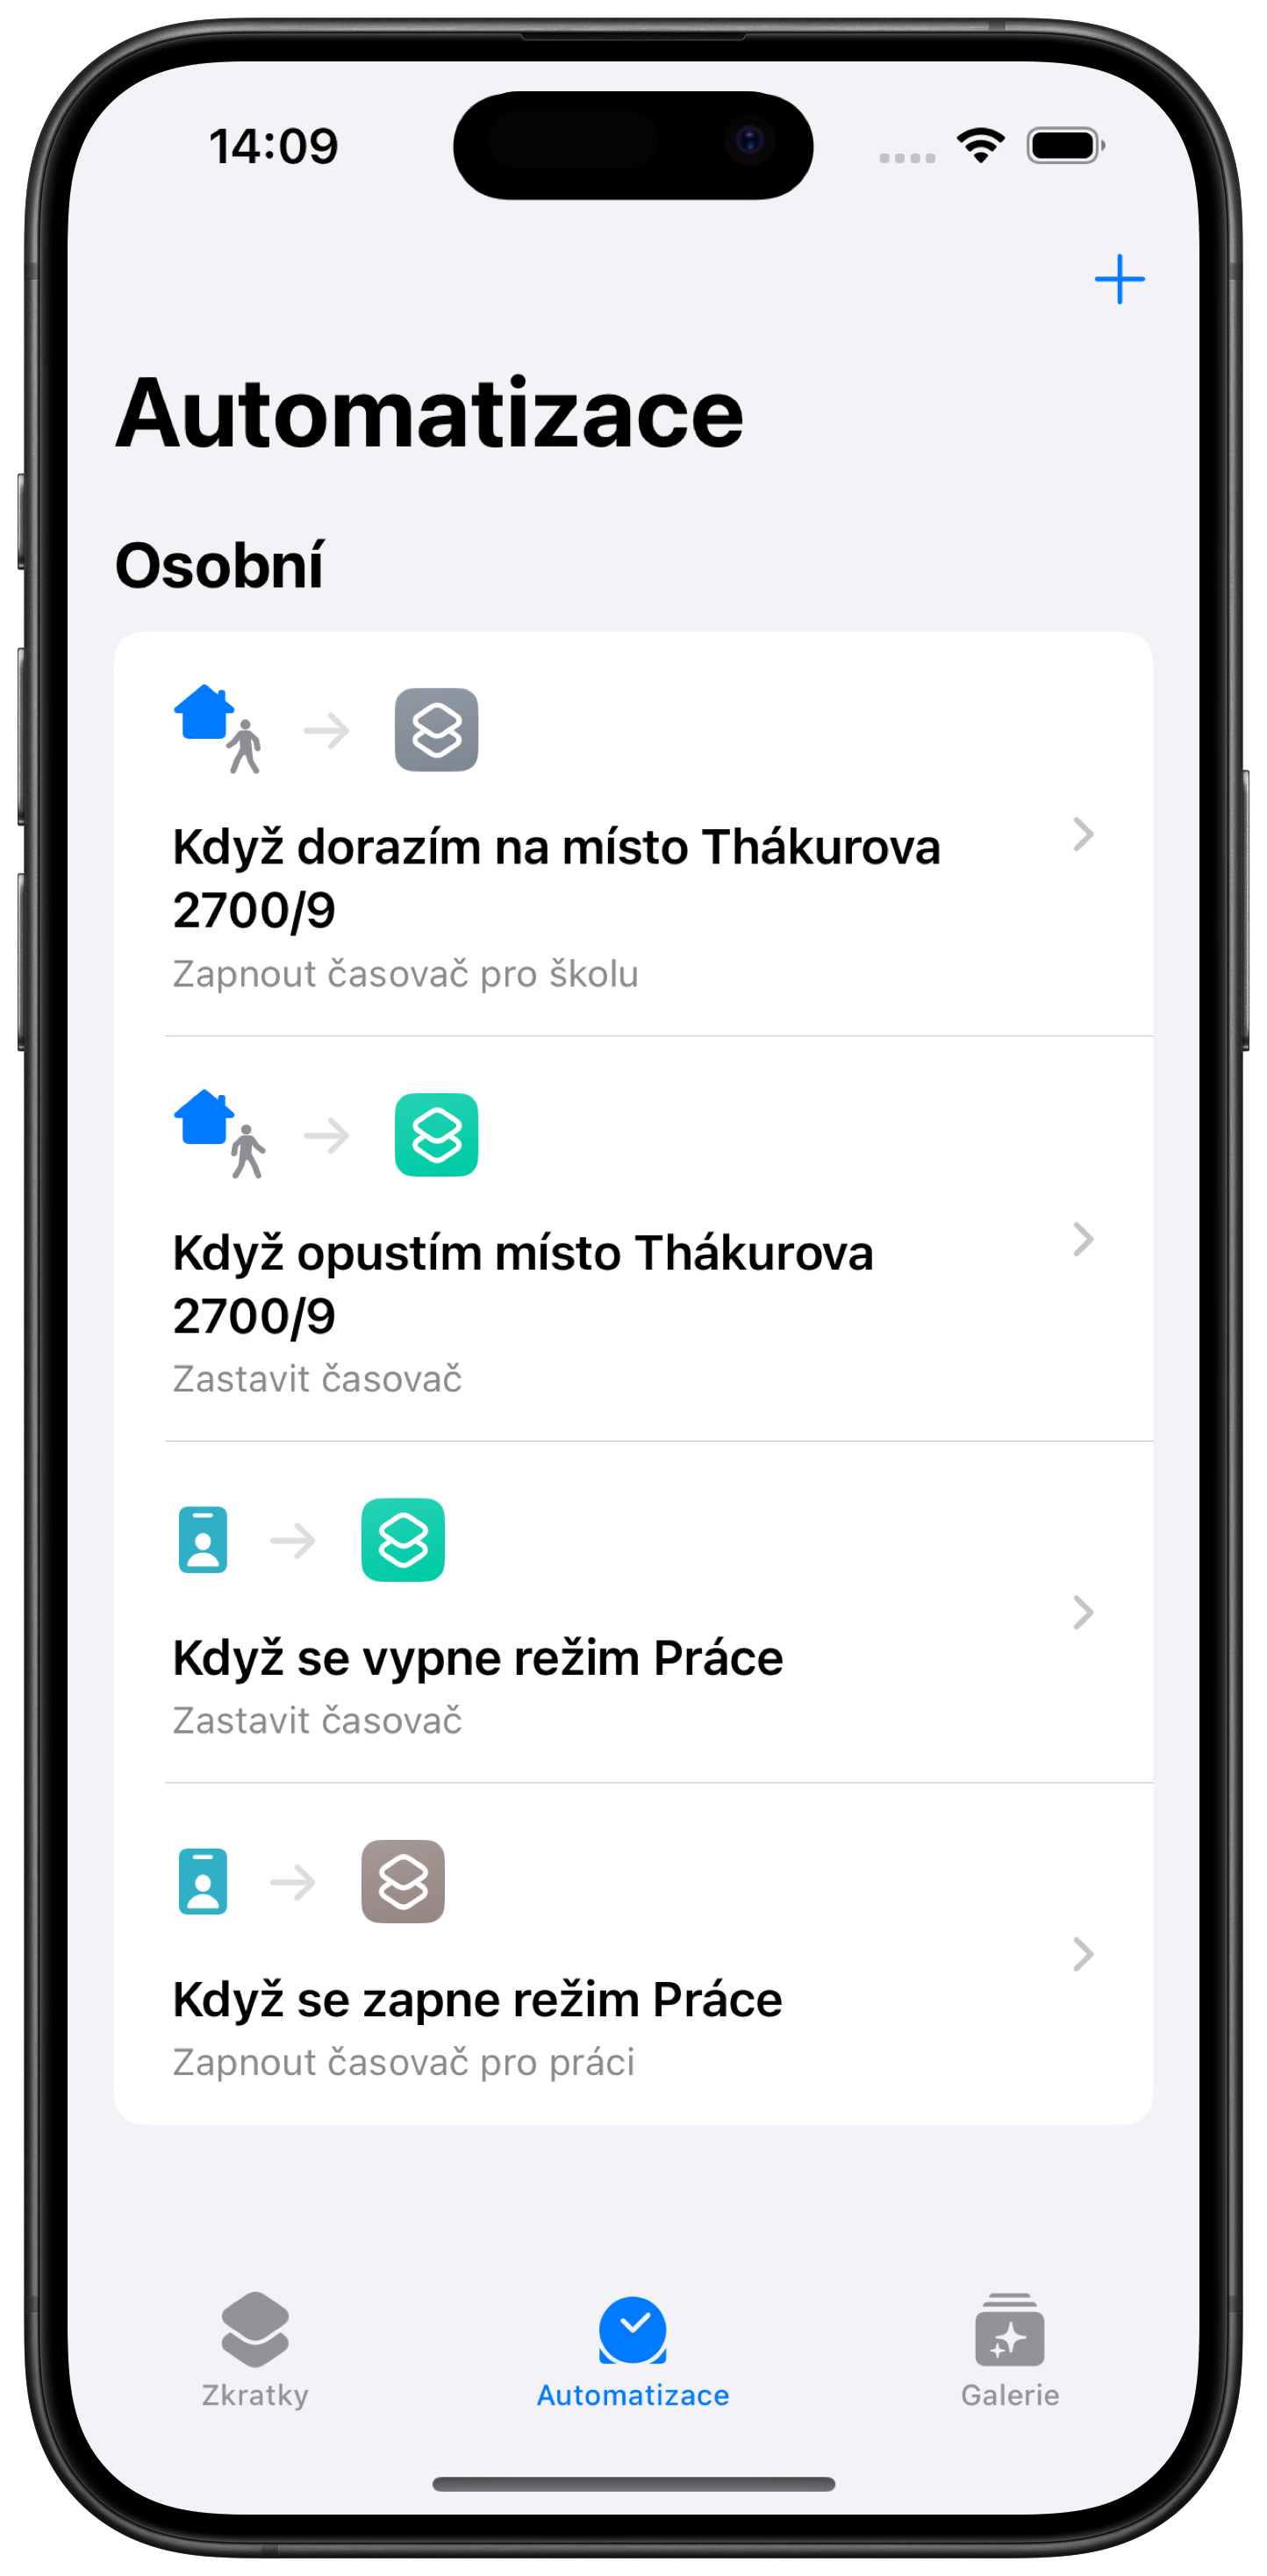
\includegraphics[width=6cm]{automations-list-impl.png}
		\caption{Seznam automatizací}
		\label{fig:automations-list-impl}
	\end{subfigure}
	\caption{Automatizace}
	\label{fig:automations-impl}
\end{figure}

V~sekci \ref{feature-integration-import} bylo také zmíněno, že pro podporu interakce s~aplikací pomocí systémových zkratek je potřeba implementovat takzvané \emph{App Intents}. Tyto \emph{intents} představují nějaký úmysl uživatele, který může pomocí zkratky spustit. \cite{ios-app-intents}

Struktury pro reprezentaci \emph{App Intents} je potřeba definovat v~hlavním \emph{targetu} aplikace, nelze je definovat v~žádném balíčku, protože by pak nebyly detekovány systémem, aby se zobrazily v~aplikaci \emph{Zkratky}. Jednotlivé \emph{intents} musí implementovat protokol (rozhraní) \texttt{AppIntent}, který vyžaduje, aby \emph{intent} obsahoval minimálně název, popis a~funkci \texttt{perform()}, která se zavolá při pokusu o~provedení \emph{intentu}. \texttt{AppIntent} také vyžaduje, aby byly texty definovány jako \texttt{LocalizedStringResource}, nelze tedy použít lokalizaci definovanou v~balíčku \emph{UIToolkit}. Pro potřeby \emph{App Intents} slouží ve složce iOS projektu složka \texttt{Intents}, kde jsou definovány \emph{intenty} a~jejich entity podle funkcionalit aplikace, a~také \emph{Resources}, tedy \texttt{Localizable.strings} soubor, který bude obsahovat texty a~jejich lokalizace pro všechny \emph{App Intents}.

Ve výpisu kódu \ref{code:start-timer-intent} lze nahlédnout implementace \emph{intentu} pro zapnutí časovače. Implementace obsahuje referenci na typ \texttt{StartTimerUseCase}, který poskytuje \emph{Dependency Injection} stejným způsobem, jako ve \emph{View Models}. Dále iplementace obsahuje definici názvu, popisu a~parametrů, které daný \emph{intent} může přijímat. A~nakonec implementace obsahuje definici funkce \texttt{perform()}, která se spustí při spuštění \emph{intentu}.

\begin{listing}
\caption{\emph{App Intent} pro zapnutí časovače}\label{code:start-timer-intent}
\begin{minted}{Swift}
struct StartTimerIntent: AppIntent {
    
    // MARK: - Dependencies
    
    @Injected(\.startTimerUseCase) private var startTimerUseCase
    
    // MARK: - Required
    
    static var title = LocalizedStringResource("start_timer_intent_title")
    
    static var description = IntentDescription("start_timer_intent_description")
    
    // MARK: - Parameters
    
    @Parameter(title: "start_timer_intent_parameter_description")
    var description: String?
    
    @Parameter(title: "start_timer_intent_parameter_project")
    var project: ProjectPreviewEntity?
    
    // MARK: - Perform
    
    func perform() async throws -> some IntentResult {
        let params = StartTimerUseCaseParams(
            body: StartTimerBody(
                clientId: project?.clientId,
                projectId: project?.projectId,
                description: description
            )
        )
        try await startTimerUseCase.execute(params: params)
        return .result()
    }
}       
\end{minted}
\end{listing}

Aby mohl nějaký objekt být parametrem \emph{App Intentu}, musí splňovat požadavky protokolu \texttt{AppEntity}. Tento protokol vyžaduje po objektech, které ho implementují, aby obsahovaly proměnnou \texttt{displayRepresentation} typu \texttt{DisplayRepresentation}, která definuje, jak se daný parametr zobrazí uživateli, tedy nějaký název, případně podnázev a~obrázek. Také po objektech vyžaduje, aby implementovaly statickou proměnnou \texttt{defaultQuery}, což je další objekt, který musí implementovat protokol \texttt{EntityQuery}. Tento protokol slouží pro objekty, které definují, odkud se mají brát všechny možnosti pro výběr konkrétní instance parametru, k~čemuž slouží funkce \texttt{suggestedEntities()} a~\texttt{entities(for identifiers: [String])}.

Pro potřeby \emph{intentu} \texttt{StartTimerIntent} je potřeba entita \texttt{ProjectPreviewEntity}, která představuje objekt projektu, který si uživatel může nastavit jako parametr \emph{intentu}. Tento objekt v~podstatě reflektuje \texttt{ProjectPreview}, který se do této reprezentace umí převést. Obsahuje tedy název, název klienta a~případně typ projektu pro určení obrázku. Identifikátor tohoto objektu má strukturu \texttt{<clientID>-<projectID>}, protože je potřeba, aby měl pouze jeden identifikátor. Implementace \texttt{ProjectPreviewEntityQuery} poté získává objekty projektů přímo přes \texttt{GetProjectsUseCase} a~\texttt{GetProjectPreviewUseCase}. Ostatní \emph{intenty} žádné parametry nepotřebují.

Propagace chyb do aplikace \emph{Zkratky} funguje automaticky, protože když nějaký \emph{Use Case} vrátí chybu, tak vrátí strukturu \texttt{KMPError}, která sama umí poskytnout lokalizovanou chybovou hlášku, která se zobrazuje jak v~aplikaci, tak v~aplikaci \emph{Zkratky}.
































